\documentstyle[epic,eepic,graphicx,tabularx,mathtools,cite,subfig,caption,algorithmic]{poly3}

%\mathindent 0pt
%\documentclass{report}[10pt]
%\usepackage{fancyhdr}
%\usepackage{amssymb}
%\usepackage{geometry}
%\usepackage{makecell}
%\usepackage[pdftex]{graphicx}
%\usepackage{mathtools}
%\usepackage{multicol}
%\usepackage[mathscr]{euscript}
%\usepackage[toc,page]{appendix}
%\usepackage[T1]{fontenc}
%\usepackage{titlesec, blindtext, color}
%\usepackage{framed}
%\usepackage{color}
%\usepackage{listings}
%\usepackage{dsfont}
%\usepackage{subcaption}
%\usepackage{natbib}
%\usepackage{tabularx}
%\usepackage[table]{xcolor}
%\usepackage{fullpage}
\newcolumntype{L}[1]{>{\hsize=#1\hsize\raggedright\arraybackslash}X}
\newcolumntype{R}[1]{>{\hsize=#1\hsize\raggedleft\arraybackslash}X}
\newcolumntype{C}[1]{>{\hsize=#1\hsize\centering\arraybackslash}X}

% Format Parameters
%\setlength{\parskip}{14pt plus 4pt minus 4pt}
%\linespread{1.125}

\newcommand{\col}[2]{\text{col}(#1)_{#2}}
\newcommand{\wrap}[1]{\left(#1\right)}
\newcommand{\sbrack}[1]{\left[#1\right]}
\newcommand{\setwrap}[1]{\left\{#1\right\}}
\newcommand{\abs}[1]{\left\lVert#1\right\rVert}
\newcommand{\norm}[1]{\left\lVert#1\right\rVert}
\newcommand{\ciel}[1]{\left\lceil#1\right\rceil}
%\definecolor{gray75}{gray}{0.75}

\newcommand{\mmathcal}[1]{{\cal #1}}
\newcommand{\mmathbb}[1]{{\Bbb #1}}

\newcommand{\Bellman}{T_{\gamma}^{\pi}}
\newcommand{\BellmanOpt}{T_{\gamma}^{*}}
\newcommand{\BellmanPiOpt}{T_{\gamma}^{\pi^{*}}}
\newcommand{\expect}[1]{\emph{E}\left[#1\right]}
\newcommand{\condexpect}[2]{\expect{#1 \middle\vert #2 }}
\newcommand{\expw}[1]{\exp\wrap*{#1}}
\newcommand{\Ssize}{\abs{S}}
\newcommand{\Asize}{\abs{A}}
\newcommand{\OptV}{V^{*}}
\newcommand{\Vpi}{V^{\pi}}
\newcommand{\OptPi}{\pi^{*}}
\newcommand{\OptVpi}{V^{\OptPi}}
\newcommand{\Aspace}{\mathcal{A}}
\newcommand{\Sspace}{\mathcal{S}}
\newcommand{\linedsection}[1]{\section*{#1}\vspace{-8mm}\hrulefill}
\newcommand{\hsp}{\hspace{20pt}}
\newcommand{\ith}{\hspace{0.1mm}$i^{th}$}
\newcommand{\jth}{\hspace{0.1mm}$j^{th}$}
\newcommand{\kth}{\hspace{0.1mm}$k^{th}$}
\newcommand{\Ith}{\hspace{0.1mm}$i^{th}$\hspace{0.5mm}}
\newcommand{\Jth}{\hspace{0.1mm}$j^{th}$\hspace{0.5mm}}
\newcommand{\Kth}{\hspace{0.1mm}$k^{th}$\hspace{0.5mm}}
\newcommand{\Forall}{\hspace{1mm}\forall\hspace{1mm}}
\newcommand{\SmallThenNormal}[1]{#1}
\newcommand{\RealVec}[1]{\in \emph{R}^{#1}}
\newcommand{\RealMat}[2]{\in \emph{R}^{#1\times#2}}
\newcommand{\Real}{\Re}
\newcommand{\RRe}{\mmathcal{R}}
\newcommand{\RRealVec}[1]{\in \RRe^{#1}}
\newcommand{\RRealMat}[2]{\in \RRe^{#1\times#2}}
\newcommand{\RReal}{\RRe}
\newcommand{\InRe}[1]{\in\RReal^{#1}}
\newcommand{\EqRef}[1]{Equation \ref{eq:#1}}
\newcommand{\EqLabel}[1]{\label{eq:#1}}
\newcommand{\FigRef}[1]{Figure \ref{fig:#1}}
\newcommand{\FigLabel}[1]{\label{fig:#1}}
\newcommand{\TableRef}[1]{Table \ref{tab:#1}}
\newcommand{\TableLabel}[1]{\label{tab:#1}}
\newcommand{\Sep}{\hspace{5mm}}
\newcommand{\SSep}{\hspace{2mm}}
\newcommand{\IE}{\emph{i.e.},\hspace{1mm}}
\newcommand{\EG}{\emph{e.g.},\hspace{1mm}}
\newcommand{\DotProd}[2]{\DotBrack*{#1,#2}}
\newcommand{\DiagMat}[1]{\text{diag}\wrap{#1}}
\newcommand{\Maps}[3]{ #1 \hspace{2mm} \Real^{#2} \rightarrow \Real^{#3}}
\newcommand{\Normalize}[1]{\frac{#1}{\norm{#1}}}
\newcommand{\Sig}[1]{\text{sig}\wrap{#1}}
\newcommand{\Unit}[1]{\emph{U}\wrap{#1}}
\newcommand{\Skew}[1]{\emph{S}\wrap{#1}}
\newcommand{\ForI}{ \forall i \in \SetWrap*{1,2,3,4} }
\newcommand{\Half}{0.5}
\newcommand{\Where} {\noindent where}
\newcommand{\SectionLabel}[1]{\label{sec:#1}}
\newcommand{\SectionRef}[1]{Section \ref{sec:#1}}
\newcommand{\SectionRefH}[1]{Section #1}
\newcommand{\SectionsRefH}[1]{Sections #1}
\newcommand{\SectionHead}[1]{\normalsize}
\newcommand{\SectionTail}[1]{\SectionLabel{#1}\normalsize}
\newcommand{\Project}[2]{{P}_{#2}\wrap{#1}}
%\newcommand{\Markup}[1]{ {\noindent\color{red}#1} }
\newcommand{\Markup}[1]{#1}
\newcommand{\NeedsRef}[1]{\Markup{Needs Ref : \emph{#1}}}
\newcommand{\MissingRef}{\Markup{[*]}}
\newcommand{\MissingFig}{\Markup{[NEED FIG]}}
\newcommand{\CaseIf}{ \text{if}\hspace{1mm}}
\newcommand{\Sum}[3]{\sum_{#1=#2}^{#3}}
\newcommand{\Para}[1]{\indent{#1}\\}
\newcommand{\R}[2]{R_{#1}\wrap{#2}}
\newcommand{\SQuotes}[1]{`#1'}
\newcommand{\DQuotes}[1]{``#1''}
\newcommand{\InlineSeg}{\SSep , \SSep}
\newcommand{\convhull}[1]{\text{conv}\wrap{#1}}
\newcommand{\zcomp}[1]{\sbrack{#1}_{z}}
\newcommand{\ycomp}[1]{\sbrack{#1}_{y}}
\newcommand{\xcomp}[1]{\sbrack{#1}_{x}}


%% Image Settings
\newcommand{\ImageWidthRatio}{1.00}
\newcommand{\ImageWidthRatioSmall}{0.400}
\newcommand{\ImageWidthRatioSub}{0.950}
\newcommand{\ImagePostNoGap}{\vspace{-2mm}}
\newcommand{\SetImage}[2]{\fbox{\includegraphics[width=#1\textwidth]{#2}}}


% Equations
%\DeclareMathSizes{4}{4}{2}{2}


% Title Formatting
%\titleformat{\chapter}{\vspace{-40mm}\Huge\bfseries}{\thechapter\hsp\textcolor{gray75}{|}\hsp}{0pt}{\Huge\bfseries}


\input{epsf}

% Override the double parenthesis
\newtagform{defaultoveride}{}{}
\usetagform{defaultoveride}


%%%%%%%%%%%%%%%%%%%%%%%%%%%%%%%%%%%%%%%%%%%%%%%%%%%
\renewcommand{\baselinestretch}{1.6}
\newtheorem{theorem}{Theorem}[chapter]
\newcommand{\btheorem}{\begin{theorem}\rm}
\newcommand{\etheorem}{$\diamond$\end{theorem}}
\newtheorem{definition}{Definition}[chapter]
\newcommand{\bdefn}{\begin{definition}\rm}
\newcommand{\edefn}{\end{definition}}
\newtheorem{lemma}{Lemma}[chapter]
\newtheorem{remark}{Remark}[chapter]
\newcommand{\bremark}{\begin{remark}\rm}
\newcommand{\eremark}{\end{remark}}
\newtheorem{example}{Example}[chapter]
\newcommand{\bexample}{\begin{example}\rm}
\newcommand{\eexample}{\end{example}}
\newtheorem{assumption}{Assumption}[chapter]
\newcommand{\bassump}{\begin{assumption}\rm}
\newcommand{\eassump}{\end{assumption}}
\begin{document}
\title{Design and Control of the BlueFoot Platform : \\ A Multi-terrain Quadruped Robot }
\author{Brian Cairl}
\date{May, 2015}
\committee{Copy Number:}
\mstitlepage
\topmargin=0.4in
\textwidth=6.0in
\textheight=9.0in
\chapter*{VITA}
\setcounter{page}{1}
	\vitaentry{Mar 23, 1992}{Born}
	\vitaentry{Jun, 2010}{Graduated salutatorian from Walt Whitman High School.}
	\vitaentry{Sep, 2010}{Entered the NYU Polytechnic School of Engineering as a Mechanical Engineering major and an Honors student.}
	%\vitaentry{Jan, 2012}{Switched to an Electrical Engineering major. Registered as a BS/MS student.}
	%\vitaentry{May, 2012}{Entered the Controls/Robotics Research Laboratory as an undergraduate researcher. Began formal design of BlueFoot's predecessor, the GreenFoot Platform.}
	\vitaentry{Jun, 2012}{Completed a minor in Mechanical Engineering.}
	%\vitaentry{Jan, 2013}{Completed undergraduate Senior Design I under the advisement of Professor Farshad Khorrami.}
	%\vitaentry{Oct, 2014}{Submitted a paper to the 2015 International Conference on Robotics and Automation (ICRA) summarizing the design and control of the BlueFoot platform .}
	%\vitaentry{Mar, 2015}{Submitted a paper to the 2015 International Conference on Intelligent Robots and Systems (IROS) on a NARX Neural Network trunk leveling controller for legged robots .}
	%\vitaentry{May, 2013}{Admitted into the 2013 NYU Undergraduate Summer Research program under the advisement of Professor Farshad Khorrami. Began formal design of the BlueFoot Platform.}
	%\vitaentry{May, 2014}{Admitted into the 2014 NYU Undergraduate Summer Research program under the advisement of Professor Farshad Khorrami.}
	%\vitaentry{Sep-Oct, 2014}{Wrote a paper on the design and preliminary control of the BlueFoot Platform, which was submitted to ICRA2015. }
	%\vitaentry{Feb-Mar, 2014}{Wrote a paper on the neural-network based platform-leveling control of legged platforms, which was submitted to IROS2015.}
	\vitaentry{Apr, 2015}{Admitted to the  NYU Polytechnic School of Engineering as PhD Fellow under the advisement of Professor Farshad Khorrami.}
	\vitaentry{May, 2015}{Received BS/MS Degrees from the NYU Polytechnic School of Engineering as an Honors Student.}
\setcounter{page}{1}
\pagenumbering{roman}
%%%%%%%%%%%%%%%%%%%%%%%%%%%%%%%%%%%%%%%%%%%%%%%%%%%



%%%%%%%%%%%%%%%%%%%%%%%%%%%%%%%%%%%%%%%%%%%%%%%%%%%
\include{publications}
\clearpage
%\chapter*{Acknowledgments}
\vspace*{\fill}
	\begin{center}
		\begin{minipage}{\textwidth}
			{\begin{center}{\textbf{ACKNOWLEDGEMENTS}}\end{center}\vspace{10mm}}

			I would like to thank Professor Farshad Khorrami for his advisement throughout the course of this project, as well as for his help in guiding my path of study in the fields of controls and robotics during my career as a BS/MS student. The knowledge and skills I have gained under Professor Khorrami's advisement will be invaluable to my future work and continued learning. %I also thank Professor Khorrami the time he spent helping me revise papers and discussing each stage of my project. My time under his advisement has given me a wealth of insight about controls, robotics, and research.
			
			\vspace{5mm}
			\hspace{5mm} 
			I would also like to thank Dr. Krishnamurthy for his guidance in various implementation matters and providing me with invaluable insight to particular problems that I faced during the course of my work. Additionally, I would like to thank my colleague Griswald Brooks for numerous instances of assistance with hardware-related matters during the design and construction of my robot. 
		\end{minipage}
	\end{center}
\vfill % equivalent to \vspace{\fill}
\clearpage

\section*{Abstract}

	This thesis presents the development and control of a small-scale quadruped robot platform with 16 actuated degrees-of-freedom, named ``BlueFoot." The BlueFoot platform has been developed for the purpose of studying multi-terrain navigation and gait control in concert with full-body actuation, which may be used for reorienting payloads (e.g., laser distance sensor and vision-sensor peripherals). This thesis will detail the design of the BlueFoot platform and its hardware sub-systems; an in-depth analysis of the system's kinematic model and robot dynamics; core Central-Pattern Generator (CPG) based gaiting algorithms introducing reflexive, feedback-driven mechanisms; and a unique foot placement and Zero-Moment Point (ZMP) posture controller based on a virtual force model and a posture feedback loop utilizing inertial measurements. %Lastly, this paper will include results from an object tracking task performed by the BlueFoot platform which utilizes a full-body actuation controller to track a moving target object through a combination of body pitch and roll adjustments, and omni-directional gaiting. 

	Following the topic of gait control, this thesis offers a method for disturbance rejection and constant orientation of the trunk of a multi-legged (here a quadruped) robot. This is significant when payloads (such as cameras, optical systems, armaments) are carried by the robot.  The trunk is stabilized by the utilization of an on-line learning method to actively correct the open-loop gait generated by a central pattern generator (CPG) or a limit-cycle method. The learning method is based on a Nonlinear Autoregressive Neural Network with Exogenous inputs (NARX-NN)-- a recurrent neural network architecture typically utilized for modeling nonlinear difference systems. A supervised learning approach is used to train the NARX-NN. 
	%The input to the neural network includes states of the robot legs, trunk attitude and attitude rates, and feet contact forces. The neural network is used to generate the total torque imparted on the robot. This approach allows on-line learning of the internal forces and disturbances due to various effects to be estimated/learned with the neural network for implementation in an inverse dynamics/computed torque controller. The controller is utilized to achieve a stable trunk (\IE a constant orientation of the trunk). 
	The efficacy of the proposed approach is shown in detailed simulation studies of a quadruped robot. 

	Lastly, this thesis will present several algorithms related to navigation control, terrain modeling, and rough-terrain gait planning. In particular, algorithms for surface reconstruction and foothold planning over uneven terrain will be integral components for future developements related to the BlueFoot project. Results from simulations and actual robot trials will be presented to demonstrate the performance of these control elements. 
\tableofcontents
\listoffigures
\listoftables
\newpage
\setcounter{page}{1}
\pagenumbering{arabic}
%%%%%%%%%%%%%%%%%%%%%%%%%%%%%%%%%%%%%%%%%%%%%%%%%%%
	%%%%%%%%%%%%%%%%%%%%%%%%%%%%%%%%%%%%%%%%%%%%%%%%%%%%%%%%%%%%%%%%%%%%%%%%%%%%%%%%%%
%%% Introduction
%%%%%%%%%%%%%%%%%%%%%%%%%%%%%%%%%%%%%%%%%%%%%%%%%%%%%%%%%%%%%%%%%%%%%%%%%%%%%%%%%%
\chapter{Introduction}
	\label{ch::introduction}
	
	\begin{figure}[h!]
		\centering
		\fbox{\includegraphics[width=\textwidth]{on_the_rocks2.jpg}}
		\caption{The BlueFoot Quadruped Robot}
		\label{fig::bluefoot_glamour}
	\end{figure}

		The design of legged robots and associated methods of locomotion control has been an area of interest spanning the past several decades, as shown by \cite{McGhee1965,Hodgins1991,Altendorfer2001,Kolter2008,Wieber2015}. Quadruped robotic systems have gained popularity in studies pertaining to variable terrain navigation and full-body stability adaptation. Well known examples of this from the past 15 years are the Tekken \cite{Fukuoka2003}, Kolt \cite{Estremera2006}, BigDog \cite{BigDog2008}, and HyQ \cite{Semini2010_PHD} quadrupeds. Many of these systems have been implemented on a larger scale so that they can carry substantial payloads while maintaining adequate system bandwidth for fast gaits and robustness to rough terrains. Few, however, have been implemented on the scale of a hobby-robot platform while still maintaining an aptitude for rough terrain navigation and comparable sensory prowess.

		The BlueFoot quadruped is a self-contained, fully-actuated platform with the dexterity to perform stabilization and repositioning maneuvers on variable terrains along the same lines as the LittleDog platform \cite{Rebula2007}. Namely, BlueFoot has been designed with 16 actuated degrees of freedom to allow for the execution of a wide range of body and leg articulations. Moreover, BlueFoot's range of articulation allows it to take on a large range of poses during motion. This level of dexterity grants the BlueFoot platform the several notable abilities, including the ability to overcome raised or uneven terrain. Additionally, BlueFoot can articulate (\IE pitch and yaw) its on-board vision sensors, which are mounted to its trunk (main body), by reposing using aggregate leg motion controls. BlueFoot also includes a sizable array of other on-board sensors for feedback and control, including joint position, velocity and loading sensors; an inertial measurement unit (IMU); and foot-contact sensors. Using the computational, sensory and motor capacities at hand, BlueFoot has the ability to utilize similar control mechanisms to those implemented on larger quadruped systems. 

		The BlueFoot platform inherently demands a variety of control routines to achieve locomotion and system stability, making this robot an ample platform for studies related to gait design and motion planning. In particular, BlueFoot's controller considers the systems kinematic model; and involves open-loop gait design and stabilization for the purpose of achieving dynamic locomotion control. In particular, BlueFoot is gaited via a central pattern generator (CPG) based gaiting technique which is augmented with a foothold controller along the same lines as \cite{Ajallooeian2013} and \cite{Rutishauser2008}. Additionally, active platform stabilization is performed via a zero-moment point (ZMP) based body placement controller which stabilizes the system using planar trunk motions during arbitrary gaiting sequences. Both such controllers make use of virtual-forces to drive system reference commands. These controller make significant use of the system's forward kinematic model for the purpose estimating the positions of the robot's joints and feet. Finally, outer-loop control routines are implemented to supply commands and corrections used in system navigation control. Among these controllers are a potential fields navigation controller which incorporates image features as targets to track; and 3D point-cloud processing routines for surface reconstruction and foot-placement planning.

	\section{Central Pattern Generators for Gait Control}

		As previously mentioned, BlueFoot's core gaiting routine relies on the utilization of artificial CPG's, which are inspired from biological neural networks which generate rhythmic motions \cite{Ijspeert2008}. \cite{Arena2000} describes biological CPGs as a form of self-organizing cellular neural network, and also explains the a the role of limited feedback in CPG networks. In fact, a key feature of these networks is that they can act without explicit sensory feedback inputs or directions from a higher-level command unit, such as a brain. Instead, signals emanating from independent motor units (and, sometimes, feedback gathered from sensory neurons) are utilized to trigger or inhibit a sequence of successive, self-coordinated motor operations. These activation sequences create loops which give rise to cyclic motion patterns. 

		In robotics, biological CPG's have inspired an artificial counterpart in which neural units are represented by multi-state unit-oscillators. The dynamics of each unit oscillator in an artificial CPG network are design to effect the dynamics of other oscillators within the artificial CPG network though tunable coupling parameters. Typically, the CPG network is implemented on a digital controller, which numerically integrates the dynamics each neural oscillator. The output states of each unit-oscillator are used to drive selected degrees of freedom of a robot system. Oscillator outputs could also be used for planning periodic motions in the robot's task space, which are then translated into the joint-space references via an inverse kinematics mapping, as is done in BlueFoot's gait control routine. The specific motions produced using the CPG are designed by careful tuning of oscillator coupling, which incurs particular phase offsets between the individual limit-cycles of each unit-oscillator. The ability to coordinate unit-oscillator dynamics is what allows artificial CPGs to be used in the control of higher-level motor tasks, such as walking or crawling.

		The selection of a unit-oscillator for use in a CPG network is a fundamental matter of CPG network design. CPG networks can be designed to employ unit-oscillator with varying oscillator dynamics (\IE varying number of states, tuning parameters, etc)which exhibit different limit-cycle behaviors. Hopf Oscillators, as used in BlueFoot CPG implementation and \cite{Righetti2006,Rutishauser2008,Matos2010}, and Van der Poll Oscillators, as detailed in \cite{Ijspeert2008}, have been applied existing CPG implementations, among other limit-cycle oscillator designs, such as the Matsuoka Neural Oscillator \cite{Endo2004}.

		Studies dealing specifically the application of CPG's to multi-legged robot gaiting (specifically quadruped, hexapods and octopodal robots) have been carried out by \cite{Arena2001,Klaassen2002,Arena2004,Inagaki2003,Inagaki2006,Billard2000,Brambilla2006,Buchli2006,Tsujita2001,Tsujita2004}.  In particular, \cite{Ijspeert2008} states that the attractiveness of CPG's in the control of legged robot locomotion lies in the ability to decouple robot motor control, \IE walking, from higher-level planning, such as navigation and body-posture control. Additionally, CPG's offer an effective way for smoothly switching between gaiting patterns, such as walking, trotting, or pacing, simply through the modification of a few control parameters. Moreover, the application of artificial CPG's greatly reduces the dimensionality of the gaiting control problem for legged robots. 

		The specific CPG controller employed in controlling the BlueFoot robot allows for the generation of coordinated motions which can be modified to yield different overall motion patterns without explicit modification of each degree of freedom employed in gait execution. Namely, CPG outputs are mapped to stepping trajectories in the robot task-space. As previously mentioned, these task-space references are mapped into joint reference positions using an IK solution for the entire robot. This approach gives way to a hybrid gaiting mechanism which combines the conveniences of CPG-based gaiting with the explicitness of strict foot trajectory planning and execution. In BlueFoot's control scheme, foot-placement is prescribed via a separate planning mechanism which decoupled from the CPG gait controller. This controller hybridization allows the CPG-based motion generator to be applied to gaiting over varying terrains.

		Another important aspect of the CPG-based gait design applied to the BlueFoot platform is the incorporation of feedback mechanisms which modify the aforementioned CPG parameters. The use of feedback to modify the CPG network for the purpose of improving gaiting stability was inspired, in part, by the work of \cite{Fukuoka2003,Endo2004}. Namely, BlueFoot's CPG based gait generation incorporates inertial feedback signals into its CPG mechanism by using them to modify oscillator amplitudes and modulate unit-oscillator frequencies. 

		Because CPG-based gaits are inherently open-loop motion control routines, a combination of axillary mechanisms must be used in concert with the CPG gait controller in order to ensure system stability during gaiting. The incorporation of feedback signals to modify CPG parameters aids in achieving this to some degree, but is usually insufficient for stable walking over largely uneven terrains.  Additionally, this method requires very careful parametric tuning to work robustly under a larger variety of terrain conditions. Thus, other means of stabilization have been incorporated into BlueFoot's gaiting routine to aid in stability. 

		In particular, BlueFoot's core stabilization routines make use of a concept named \emph{artificial synergy synthesis} in which gaiting is carried out independently of a stabilization control. Namely, body stabilization is performed by a smaller set of the robot's degrees of freedom while gaiting is carried out independently by the remaining \cite{Vuko1972,Yamaguchi1993}. In the original implementation of this technique, adaptations to trunk motion are utilized to stabilize the overall motion of the robot utilizing a ZMP-based approach while gaiting is controlled by a fixed-motion routine. Here, body and foot-placement are both controlled as independent, dynamic processes. The outputs of each controller are used to specify body and foot placement in the robot task space. These commands are combined using the robot's inverse kinematics solution, which generates a final set of angular references which are used to control servo motors at each joint.




	\section{Zero Moment Point Body Placement Control}

		The zero-moment point (ZMP), which is equivalent to the center of pressure (CoP), is formally defined as the point on the ground beneath a walking system at which the net moment acting upon the trunk (referred to as the tipping moment) is zero \cite{Sardain2004}. The concept of ZMP and its application to legged robotics was originally introduced by \cite{Vuko1972} and expanded upon in \cite{Goswami1999}, both of which describe ZMP theory towards the control of biped robots.

		Formally, the ZMP, denoted $p_{ZMP}$, can be defined using a formulation for the CoP wherein the moments about $\tau_{x}$ and $\tau_{y}$, the lateral tipping-moments applied to the robot's body in the world frame, are equal to zero. The solution for $p_{ZMP}\in\Re^{3}$, with respect to a set of $N$ foot contact points $p_{i,e}\in\Re^{3}$ and $N$ associated applied foot-contact forces $f_{i,e}\in\Re^{3}$, arises as a bounded set of solutions to the equation
			\begin{equation}
				\sum^{N}_{i=1}\wrap{p_{i,e}-p_{ZMP}}\times f_{i,e} 
				= 
				\left[
					\begin{array}{c}
						\tau_{x}	\\
						\tau_{y}	\\
						\tau_{z}
					\end{array}
				\right]
				=
				\left[
					\begin{array}{c}
						0			\\
						0			\\
						*
					\end{array}
				\right]
			\end{equation}
		where $z$-coordinate of $p_{ZMP}$, $\zcomp{p_{ZMP}}$, is strictly zero when the walking surface is flat, as shown in \cite{Wieber2015}. Here, derivations for flat-surface ZMP motion will be described, but equations associated with this technique can be extended non-flat terrain motion in a straight-forward way. The following expression is derived from dynamical equations which describe the total angular momentum, $\dot{L}$, about the legged system's center of gravity (COG), $p_{COG}$:
			\begin{equation}
				\dot{L} = \sum_{i=1}^{N} p_{i,e}\times f_{i,e} - m_{T} p_{COG} \times \wrap{ \ddot{p}_{COG} + \vec{g} }
			\end{equation}
		where $m_{T}$ is the total mass of the legged system and $\vec{g}$ is the standard gravity vector. Assuming that all foot-contacts exist on a flat plane, \IE $\zcomp{p_{i,e}}=0\SSep \forall i=[1,...,N]$, and all contact force, $f_{i,e}$ are pointing upward, the $p_{ZMP}$ of the system can be written as
			\begin{equation}
				p_{ZMP} 
				= 
				\frac{ \sum_{i=1}^{N} \wrap{ p_{i,e} \times f_{i,e} } }{ \sbrack{\sum_{i=1}^{N} f_{i,e}}_{z} }
				= 
				\frac{ 	p_{COG} \times \wrap{ \ddot{p}_{COG} + \vec{g} } + \dot{L}m_{T}^{-1} }{ \zcomp{ \ddot{p}_{COG} + \vec{g} }}
				\in \mmathcal{C}_{ZMP} 
			\end{equation}
		where
			\begin{equation}
				\mmathcal{C}_{ZMP} = \convhull{p_{1,e},p_{2,e}...,p_{N,e}}
			\end{equation}
		with $\text{conv}(*)$ defining a convex hull generated from a set of input points, $(*)$. $\mmathcal{C}_{ZMP}$ is used to represent the solution space of $p_{ZMP}$. Moreover, $\mmathcal{C}_{ZMP}$ places a bound on the angular momentum $\dot{L}$ which results from contact variations presented through $p_{i,e}$ and $f_{i,e}$. Setting $\dot{L}=0$, a condition is defined for zero tipping. For BlueFoot's ZMP controller formulation, it is also assumed that the acceleration of the COG is sufficiently small, \IE $\ddot{p}_{COG}\approx0$ which yields the following, intuitive condition for minimal tipping:
			\begin{equation}
				\norm{p_{ZMP} - p_{COG}} < \epsilon
			\end{equation}
		where $\epsilon$ is a scalar bounding constant. Thus, the general idea of this ZMP-based controller is to compute an approximate ZMP location and place the center of the robot's trunk (described by the translation $p_{b}$) such that the platform's COG approaches its associated ZMP for some arbitrary kinematic configuration. This is done in an effort to reduce $\norm{\dot{L}}$, so as to avoid tipping about the contacting feet.







	\section{Trunk stabilization}

		In addition to the aforementioned task-space controllers, a learning controller, which features the use of a NARX neural network is used to aid trunk stability has been studied. In essence, this controller learns to approximate disturbance dynamics during periodic gait routines and corrects trunk orientation by administering adaptations to joint position controls. The goal of such control routine is to achieve a level trunk during locomotion.
		
		\begin{figure}[h!]
			\centering
			\fbox{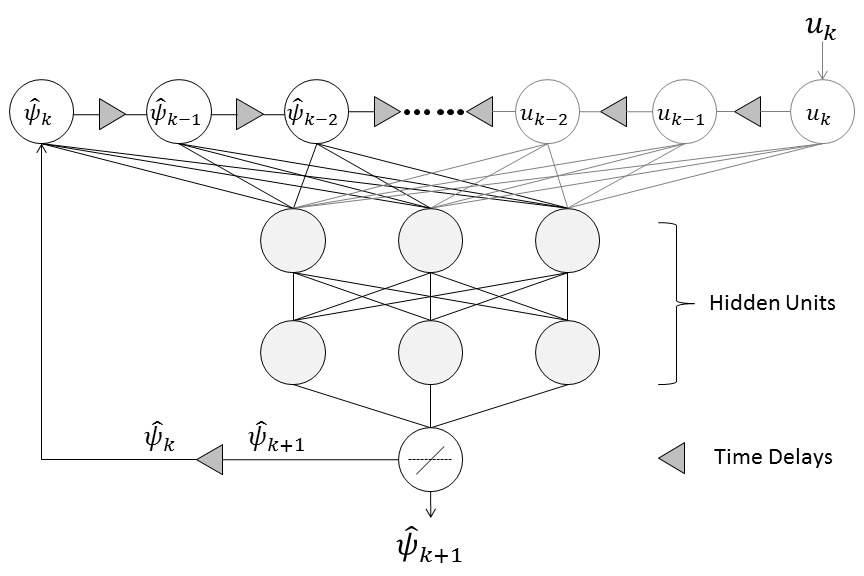
\includegraphics[width=1.0\textwidth]{narx_network_diagram.png}}
			\caption{Parallel NARX-network model with a linear output layer.}
			\label{fig::narx_net}
		\end{figure}

		A NARX-NN architecture is used in this controller because of  its known effectiveness in approximating nonlinear difference systems and making multivariate time-series predictions \cite{Tsungnan1996,ChenBillings1990,Hihi1996,Billings2013}. Moreover, the NARX-NN is a natural fit for a problem of this nature where the dynamics being considered are both periodic and of a high enough complexity where a nonlinear approximation method is warranted. The parallel NARX-NN model, shown in Figure \ref{fig::narx_net}, is comprised of a feed-forward neural network whose input layer accepts a series of time-delayed system state values and network-output histories. The NARX-NN is trained to predict system states in the next time-instant from these inputs. Conveniently, NARX-NN training can be performed using standard BP because recurrence occurs between network inputs and outputs, and not within the hidden layers \cite{Nelles2001}.

		The NARX-NN is trained to capture the effects of forces and moments and dynamical couplings that act on the trunk so that an appropriate torque input to the joints is computed to reduce such effects on trunk orientation while performing the gate. This is achieved by considering the inverse dynamics corresponding to joint motion.

		Disturbances imparted upon the trunk during gaiting manifest in the term $\Phi$, largely as a result of variations in $f_{ext}$ and associated effects due to dynamical coupling. Because of this, the NARX-NN will learn an estimate for $\Phi$, denoted $\hat{\Phi}$. The network is trained on-line using the standard incremental back-propagation (BP) algorithm with an adapted learning rate, $\gamma^{lr}$ and momentum term, $\mu$ \cite{Rumelhart1988,Rumelhart1995}. This error BP algorithm is a gradient-descent based method used to train a feed-forward neural network with $n$-layers and layer-connection matrices $\setwrap{W^{1},W^{2},...,W^{n-1}} \in \emph{W}$. The BP algorithm, as used in this control approach, is summarized in matrix-vector form in (adapted from \cite{Rojas1996ch7}) as follows: 

		\begin{equation}
			\Delta W^{i} \leftarrow
				-\gamma^{lr} \wrap{ \frac{ \partial o^{i} }{\partial {W^{i} } }  o^{i-1} }^{T}  + \mu \Delta W^{i} = 
				-\gamma^{lr} \delta^{i} \wrap{o^{i-1}}^{T}  + \mu \Delta W^{i}
			\label{eq::bp_weight_update}
		\end{equation} 
		%
		where
		%
		\begin{equation*}
			\delta^{i} = \wrap{ \nabla_{y} \sigma^{i}\wrap{y^{i}} } e^{i}
			\label{eq::bp_error}
		\end{equation*}
		\begin{equation*}
			y^{i} = W^{i} o^{i-1}
			\label{eq::bp_error}
		\end{equation*}
		\begin{equation*}
			e^{i} =  \wrap{ W^{i} }^{T} \delta^{i+1} \hspace{2mm} \forall \hspace{2mm} i\neq n,
		\end{equation*}
%%
		$\gamma^{lr} \in [0,1]$, the learning and  $\mu \in [0,1]$, the learning momentum; $W^{i} \in \Re^{N_{O}^{i}\times N_{I}^{i}}$, which represents the weighting matrix between the \Ith layer (of size $N_{I}^{i}$ nodes) and $(i+1)^{th}$ layer (of size $N_{O}^{i}=N_{I}^{i-1}$); $\Delta W^{i}$, which represents the corresponding weight update to $W^{i}$; and $e^{i}$ is the output error for each \Ith layer. For the output ($n^{th}$) layer, $e^{n}$ is equal to the difference between the network output and the network output target, which will be defined later. For all other layers, $e^{i}$ represents a \emph{back-propagated} error. from the $(i+1)^{th}$ layer.

%%
		$\sigma^{i}(y^{i})$ is an element-wise activation function which outputs a vector of activation outputs, $\sigma_{j}^{i}(y_{j}^{i}) $ for each \Jth, weighted input, $y_{j}^{i}$, defined as follows:
			\begin{equation}
				\setwrap{ \sigma^{i}(y^{i}) = \sbrack{ \sigma_{1}^{i}(y_{1}^{i}),...,\sigma_{N_{I}^{i}}^{i}(y_{N_{I}^{i}}^{i}) }^{T} \hspace{2mm} : \hspace{2mm} \Re^{N_{I}^{i}} \rightarrow \Re^{N_{I}^{i}}}
			\end{equation}

		For the trunk-leveling controller being described, a symmetric sigmoid activation function is used as a hidden-layer activation function. Formally:
			\begin{equation}
				\sigma_{j}^{i}(y_{j}^{i}) \equiv \tanh(y_{j}^{i}) \in [-1,1]. 
				\label{eq::activation_function}
			\end{equation}
		Hence the gradient which arises for the activation mapping at each hidden layer, $\nabla_{y} \sigma^{i}(y^{i})$, is defined as follows: 
		\newcommand{\acti}[1]{1 - \wrap{\sigma^{#1}_{1}(y^{i})}^{2}}
		\begin{equation}
			\nabla_{y} \sigma^{i}(y^{i})  =
			\left[
			\begin{array}{cccc}
				\acti{1} 	&	0		&	\ldots 		&	0 			\\	
				0			&	\acti{2}&	0			& 	\vdots 		\\
				\vdots 		&	0		& 	\ddots 		& 	0			\\
					0			&	\ldots	&	0			& 	\acti{N_{I}^{i}}
			\end{array}
			\right]
			\label{eq::bp_sigmoid_deriv}
		\end{equation} 
		given the derivative properties of the $\tanh\wrap{*}$ function. For the output layer, a linear activation function is used, defined simply as:
			\begin{equation}
				\sigma^{O}(y^{O}) = y^{O} \in \Re. 
				\label{eq::output_activation_function}
			\end{equation}
		with $\nabla_{y}\sigma^{O}(y^{O})$ defined as:
			\begin{equation}
				\nabla_{y}\sigma^{O}(y^{O}) = I_{N_{I}^{O}\times N_{I}^{O}} . 
				\label{eq::bp_linear_deriv}
			\end{equation}		
		The success of this learning mechanism, as it applies to the trunk-leveling controller to be presented, is predicated on the periodicity of the system dynamics during gaiting. Like any BP-trained neural network, repetition of similar input and output sets is paramount for successful network training and, by extension, prediction accuracy. It is assumed that this specification can be met given the inherently cyclic nature of the dynamics being estimated during gaited locomotion. 




	\section{Potential-Fields Navigation}

		The method selected for navigating the BlueFoot platform over flatland is a potential-fields control approach. This approach is described in \cite{Hogan1984} for the purpose of controlling robotic manipulators, and analyzed in-depth in \cite{Koren1991}. In particular \cite{Koren1991} presents shortcomings of this approach, which will be covered in-brief later in this section. Despite its pitfalls, a potential fields navigation methods offers a relatively simple and intuitive approach to robot navigation and fits well into mobile robotic tasks which involve ``wandering'' type navigation over flat-regions. In particular, the approach is applied to navigation where the robot has yet to acquire any knowledge of surrounding obstacles. The potential fields navigation approach used to navigate the BlueFoot robot is coupled with camera-based feature tracking to guide the robot towards potential areas of interest within an immediate space, fully unknown space.

		The potential fields approach is used in mobile robot navigation by moving the robot according to a guiding virtual force-vector, $F_{nav}$ \cite{Koren1991,ArambulaCosio2004}. This vector is comprised of a sum of virtual repulsive forces, $F^{-}$ (typically generated from range-sensor data), and virtual attractive forces, $F^{+}$, which pull the robot towards known goals. Thus $F_{nav}$ formally defined as:
		%%%
		\begin{equation}
			F_{nav} = F^{+} + F^{-}
			\label{eq::sumofforces}
		\end{equation}

		The general form for the force components $F^{+}$ and $F^{-}$ (represented as $F_{c}$ in the equation which follows) is as follows:
		%%%
		\begin{eqnarray}
			d_{k} 	&=& p_{POI,k} - p_{robot} \nonumber\\
			F_{c}	&=& \alpha_{F}\sum_{k}\wrap{ f(\norm{d_{k}})\frac{d_{k}}{\norm{d_{k}}} }
			\label{eq::sumofforces}
		\end{eqnarray}	
		where $p_{poi}$ and $p_{robot}$ are position of each \Kth point-of-interest (POI) and the position of the robot platform; $f(*)$ is a potential function which returns a scalar potential factor with respect to a scalar argument $(*)$; and $\alpha_{F}$ is a scaling parameter which is positive when the POIs considered represent goals and negative when POIs represent obstacles to avoid. The potential function and scaling factors are designable for particular applications. For BlueFoot's navigation scheme, attractive and repulsive forces are generated using a consolidated, piecewise forcing function which is used to guide through an environment where a goal is not specified before hand. 

		According to \cite{Koren1991} the main pitfall with a potential fields navigation approaches as a whole is the hazard presented by local minima within the global force-field. At a local minimum, the $F^{+}$ and $F^{-}$ are of nearly equal magnitude, causing the magnitude of the total guiding force vector $F_{c}$ to be close to zero. In practice, reaching a point at which robot will be completely stationary is unlikely, as sensor readings used to observe environmental obstructions are corrupted by noise. This noise induces random perturbations in the robot's motion.

		In fact, perturbations due to sensor noise could actually aid in relieving a situation in which a robot is stuck in a local minima. However, the gradient of the force-field around a minimum point could be very steep and cover a large area around the aforementioned singularity. These type of potential-sink regions cause the robot to exhibit limit-cycle behavior as it periodically overshoots and re-attracts to minimum without ever escaping. 

		This can be overcome, in part, by adding an artificial \emph{inertia} (essentially a tunable gain parameter) to robot navigation reference signals. Doing so may cause the robot platform to sufficiently overshoot a minimum point such that it leaves the local attraction field. A more sophisticated approach is mentioned in \cite{Krishnamurthy2007}, which involves a ``stuck" detection algorithm. The idea behind such an algorithm involves a deduction about whether or not the robot is captured in a local minima based on samples of the robot’s motion state (\IE position and velocity). Once the robot has determined that is it stuck, it is instructed to execute a small random-walk as a means of escape. 

		Here, the local minima problem is addressed through the use of dynamic, auxiliary target points, as done in \cite{ArambulaCosio2004} via a hybrid navigation potential-fields / visual-servoing scheme. Instead of incorporating goal points directly into the potential fields scheme, features fir for tracking are handled using an entirely separate mode of navigation. A separate set of generated navigation commands is mixed with command generate via the base potential fields algorithm. The amount of influence either command scheme has over the final navigation command parameters, $v^{r}$ and $\omega^{r}$, depends on relative measure of ``closeness" to the object being tracked, which the robot determines in an image processing routine. The specifics of this will be describes in \ref{ch::navigation}. 

		Hence, the potential-fields portion of this control scheme is used only for the purpose of avoiding potential obstructions, sensed via LIDAR range data. Image-features are used in a visual-servoing routine which guides the robot toward features of interest which fall within the robot’s camera gaze.This approach offers the ability to manually guide the robot during navigation, by either a human overseer, or a partner robot (which could wear trackable markers), as it performs an independent obstacle avoidance routine. The advantage of this approach lives in its simplicity, as it relies only on immediate environmental samples and, thus, has relatively minimal implementation demands.  As a mechanism for partially-guided wandering-type (random) navigation within an unknown region, this approach is certainly adequate as a will be shown via empirical results from both simulation and real-world trials.




	\section{3D Surface Reconstruction for Rough Terrain Planning}

		The previously introduced navigation scheme is utilized, exclusively, for flatland navigation. As such, it relies on 2D LIDAR scans. For navigation and planning over rough terrain, knowledge of 3D surfaces in the robot’s environment (with high feature detail) must be acquired. This thesis will provide the preliminaries for rough-terrain navigation and planning by way of several surface reconstruction methods from point-cloud data. First, a method for composing 3D point clouds from successive 2D LIDAR scans will be described. Then, algorithms for generating 3D height-maps and approximate surfaces from raw point-cloud data will be described. Finally, a simple approach for planning over the perceived terrain using generated height-maps will be offered.




	\section{Overview of Thesis}

		This thesis will first detail the major hardware components; design considerations; and construction of the BlueFoot platform. Next, the software and processing architecture used to control the BlueFoot platform will be described. Thereafter, the kinematic and dynamical model of the BlueFoot system will be described, followed by control routines which are presently implemented to gait, stabilize, and navigate the BlueFoot platform. The final section of this thesis will contain concluding statements about the system's design and control, including remarks about possible future directions of study related to the BlueFoot platform and legged robotics as extensions of the existing work.

	\label{ch::hardware_and_design}
%%%%%%%%%%%%%%%%%%%%%%%%%%%%%%%%%%%%%%%%%%%%%%%%%%%%%%%%%%%%%%%%%%%%%%%%%%%%%%%%%%
%%% Robot Hardware and Design
%%%
%%% Section 1 : Robot Design
%%% 
%%% Section 2 : Controller Configuration/Descriptions
%%%
%%% Section 3 : Sensors
%%%
%%% Section 4 : Device Connectivity Layout
%%%
%%% Section 5 : System Power
%%%		SubSection 5.1 : Power Requirements and Runtime
%%% 	SubSection 5.2 : Power Routing
%%%
%%%%%%%%%%%%%%%%%%%%%%%%%%%%%%%%%%%%%%%%%%%%%%%%%%%%%%%%%%%%%%%%%%%%%%%%%%%%%%%%%%
\chapter{Hardware and Design}
	\begin{figure}[h!]
		\centering
		\fbox{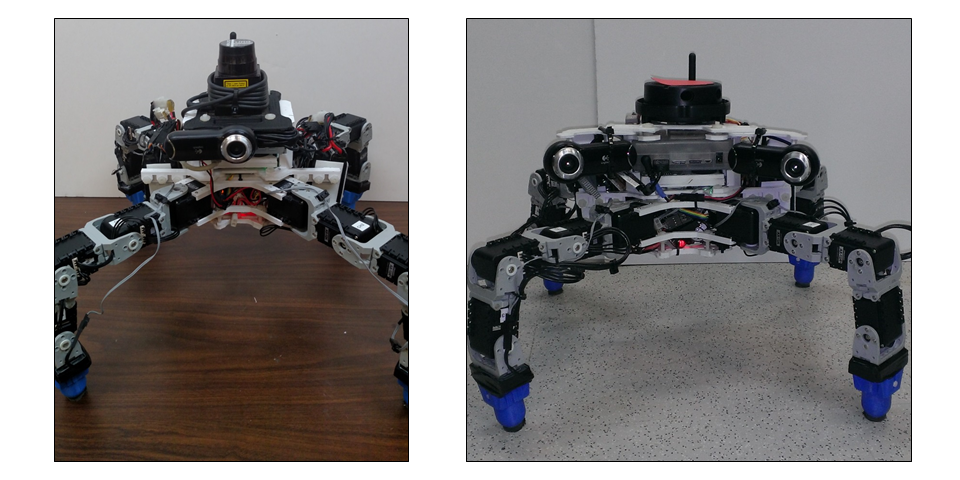
\includegraphics[width=\textwidth]{robot_selfies.png}}
		\caption{The BlueFoot Quadruped Robot: single-camera configuration \emph{(left)}; stereo-camera configuration \emph{(right)}}
		\label{fig::bluefoot}
	\end{figure}

	\section{Overview and Design Goals}
	
	The BlueFoot quadruped robot is designed as a small-scale, general-purpose legged mobile platform with enough physical dexterity and on-board computational/sensory power to perform complex tasks in variable environments. BlueFoot's hardware configuration is aimed at performing of tasks as a standalone unit, i.e. without power tethering or off-board processing. BlueFoot's sensory, computational and power-source outfit make it fit to complete tasks in both settings fully and semi-autonomous modes.

	The implementation of a legged robot which meets these general specification is inherently bottlenecked by several well-known shortcomings which plague legged robot design. These drawbacks can be summarized as follows: relatively low payload capacity, as leg joints are often subjected to substantial dynamic torque loading during gaiting; and higher power consumption due to a, typically, larger number of total actuators. Thus, a general-purpose, multi-legged system like the BlueFoot platform must ultimately achieve a balance between payload-carrying capacity (i.e. maximum joint-servo output torque); actual on-board payload; and on-board energy supply. It is desirable that the sensory and computational power; as well as overall mobility of a legged system are simultaneously maximized along with the aforementioned characteristics. 
	
	The design goals which have guided the implementation of the BlueFoot quadruped have been tailored to a yield an overall system design which is both feature rich, computationally powerful, and exploits the natural dexterity and terrain handling of legged robotic systems. Namely, the core design requirements which have guided BlueFoot's development can be summarized as follows:
		\begin{itemize}
			\item{The use of legs with joint redundancy for improved dexterity}
			\item{The use of smart servos for extended joint feedback and control}
			\item{A distributed on-board and computing architecture for hierarchal task handling}
			\item{A vision sensor array including a camera and laser-ranging sensors}
			\item{30+ minutes of total battery life}
		\end{itemize}
	
	This chapter will outline how an implementation meeting these design goals is achieved, starting with the structural layout of the system. Next, major system payloads and the associated interfacing of major devices will be described. This section which will include details about BlueFoot's actuators, computational modules, and sensory mechanisms. Lastly, the system power routine, energy requirements, and runtime will be detailed.


	\section{Robot Structure}
	
		BlueFoot's body is designed in a modular fashion and is comprised of mostly custom designed, 3D printed parts. The use of 3D printing as a fabrication method allowed for rapid design iterations the early stages of system prototyping, and has kept the weight of the robot's overall structure relatively low. Parts were mainly printed from both PLA and SLA plastics. BlueFoot's overall weight (when fully outfitted) is $1.85-1.98 \text{ kg}$, depending on configuration.

		The modularity of BlueFoot's overall structure arises from the inherent design requirements associated with 3D printing and general design practices aimed at keeping the system reconfigurable for the incorporation of updated sensory and computational hardware. Moreover, parts are designed to fit future replacements while conforming to the constraints imposed by the 3D printing fabrication method, i.e. particular part size and orientation requirements. Such constraints had to be met by each designed part to ensure print feasibility. 

		The BlueFoot platform has undergone several minor redesign phases since its inception. These redesigns were necessary to bring the BlueFoot platform to its final structural and hardware state and were performed to accommodate changes in  sensory/computational hardware. The sections that follow will mainly focus BlueFoot's final hardware configurations.

		\subsection{Main Body (Trunk) Design}
		
			BlueFoot's trunk consists of the three main sections: a lower module which interfaces the legs with the main body; a center chassis, designed to  hold computational and battery payloads; and a top platform, which interfaces the system's visions sensors to the trunk. These sections will be referred to as the \emph{Root} module, the \emph{Main} module, and the \emph{Head}module, respectively. The full trunk (not including sensor dimensions) fits within a 21.6 by 21.6 by 15.3 cm bounding box. 

			\subsubsection{The Root Module}

				\begin{figure}[h!]
					\centering
					\fbox{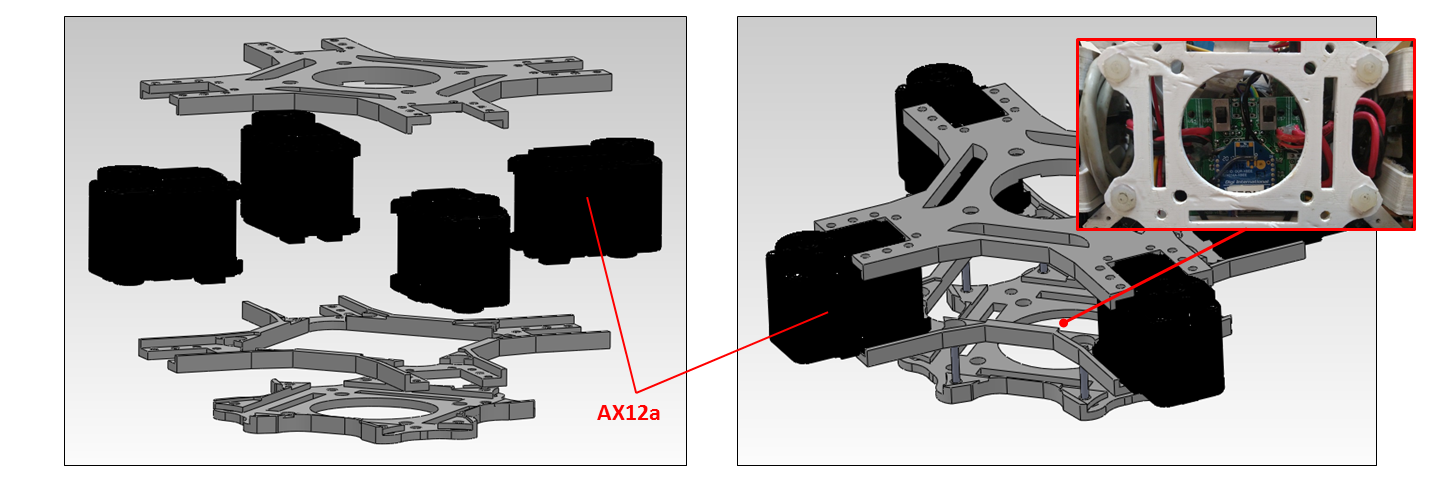
\includegraphics[width=\textwidth]{root_full.png}}
					\caption{Root section of trunk. Call-out in top-right shows main-switch access through the bottom of the root module.}
					\label{fig::root_module}
				\end{figure}

				The Root module, consists of three plates, as shown in Figure \ref{fig::root_module}. Each plate is designed with a central opening to allow for wired connections to pass to other trunk modules. Two such plates directly interface with four servos, which are mounted to four symmetric arms which extend from the center of each plate. These servos are the first joint (hip-joint) of each leg. Each servo mounts to the top a bottom plates via mounting holes located at the top and underside of each servo chassis. The assembly is mated with small steel bolts. A third, smaller plate is attached to the bottom of the module to provide more space for power components and associated wiring. This plate is attached to the bottom of the module via plastic standoffs. An opening in the middle of this plate provides access to the system's main power switches, as well as a removable XBEE wireless radio unit.

			\subsubsection{The Main Module}
		
				The Main module of BlueFoot's trunk includes compartments for an in-house designed AutoPilot unit and a main computer unit, an ODROID-XU. The Main module is designed such that the AutoPilot and ODROID-XU computer slide in and out of the body. The computer payloads are locked into position when the Head module is added to the assembly. The Main body section is designed to fit both computers when stacked upon one another, as depicted in Figure \ref{fig::main_module}. The computer stack is positioned directly in the center of the module when inserted.
%
				\begin{figure}[h!]
					\centering
					\fbox{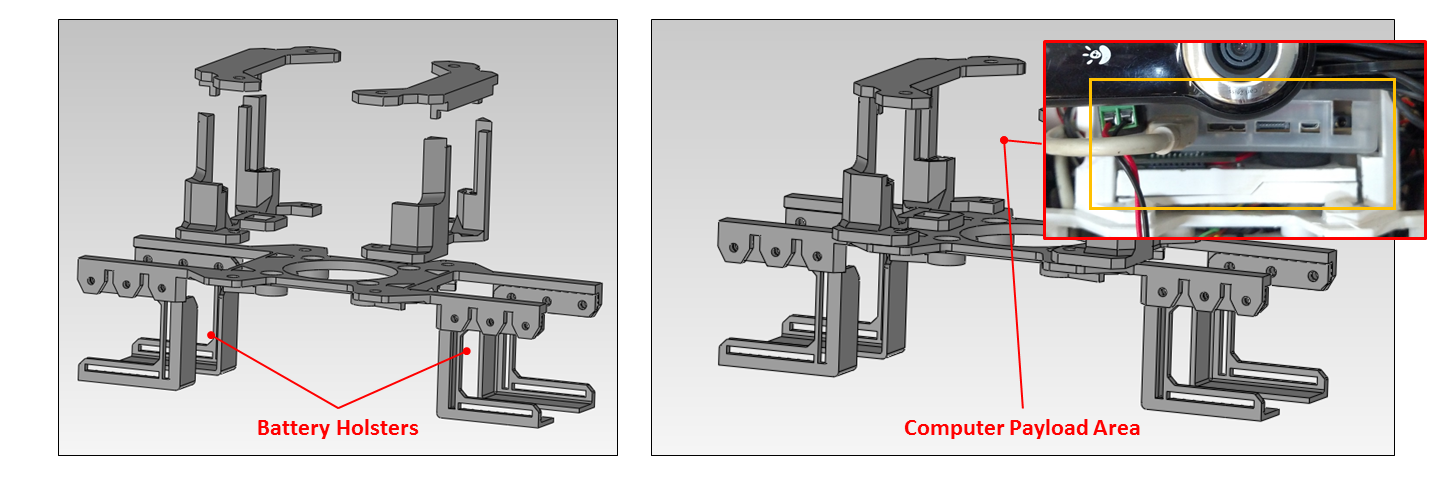
\includegraphics[width=\textwidth]{main_full.png}}
					\caption{Main section of trunk. Call-out in the top-right shows how the ODROID-XU and AutoPilot computers fit within the module.}
					\label{fig::main_module}
				\end{figure}

			
				The Main module also includes two battery holsters, which hang over its left and right sides. The holsters align the battery packs with the center of Root module. This battery placement serves to lower the center of mass (COM) of the trunk. Doing so serves to lower the magnitude of dynamic torques imparted upon the leg servos during gaiting by decreasing the net moment due to gravity imparted upon the system when the body is oriented away from the direction of gravitational force. The entirety of the Main module is attached to the Root module through the battery holster sub-assembly by four plastic bolts.
		
			\subsubsection{The Head Module}

				Two separate Head modules have been designed for the BlueFoot system : one of which features a stereo camera pair and a Piccolo LIDAR sensor (PLDS); and a monocular design, which features a camera and a Hokuyo-URG LIDAR sensor, as shown in Figure \ref{fig::head_module}. Each head module is attached to Main module via four plastic mounting screws. In the stereo-camera design, two adjustable wings are attached to either side of a top platform which hold cameras. These wings were designed to be adjustable to aid in stereo-camera configuration and calibration. The position of each camera on the trunk allows for a persistent field of view by each camera during mobilization. The PLDS unit is positioned such that the center of its rotating laser head is aligned to the center of the trunk. 

				\begin{figure}[h!]
					\centering
					\fbox{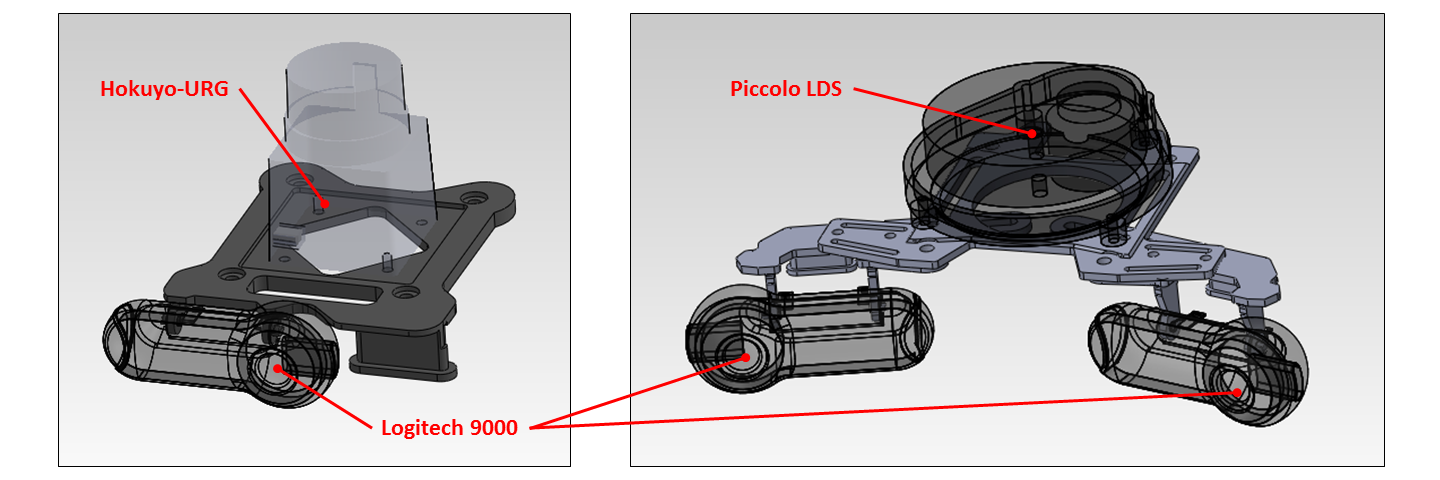
\includegraphics[width=\textwidth]{head_full.png}}
					\caption{Head section of trunk. Monocular camera configuration with Hokuyo-URG \emph{(left)}; and Stereo configuration with PLDS \emph{(right)}. }
					\label{fig::head_module}
				\end{figure}		

				In the monocular design, a single camera is mounted such that the lens of the camera is aligned to the sagittal plane of the trunk. This configuration is currently be used as BlueFoot's \emph{primary} head configuration and is mainly being used for 3D point-cloud building and surface reconstruction via 2D LIDAR scans. This is because the Hokuyo-URG laser scanner used in this configuration offers higher-resolution laser-scan outputs, which will be covered in more detail later in this chapter.

		\subsection{Leg Designs}

			\begin{figure}[h!]
				\centering
				\fbox{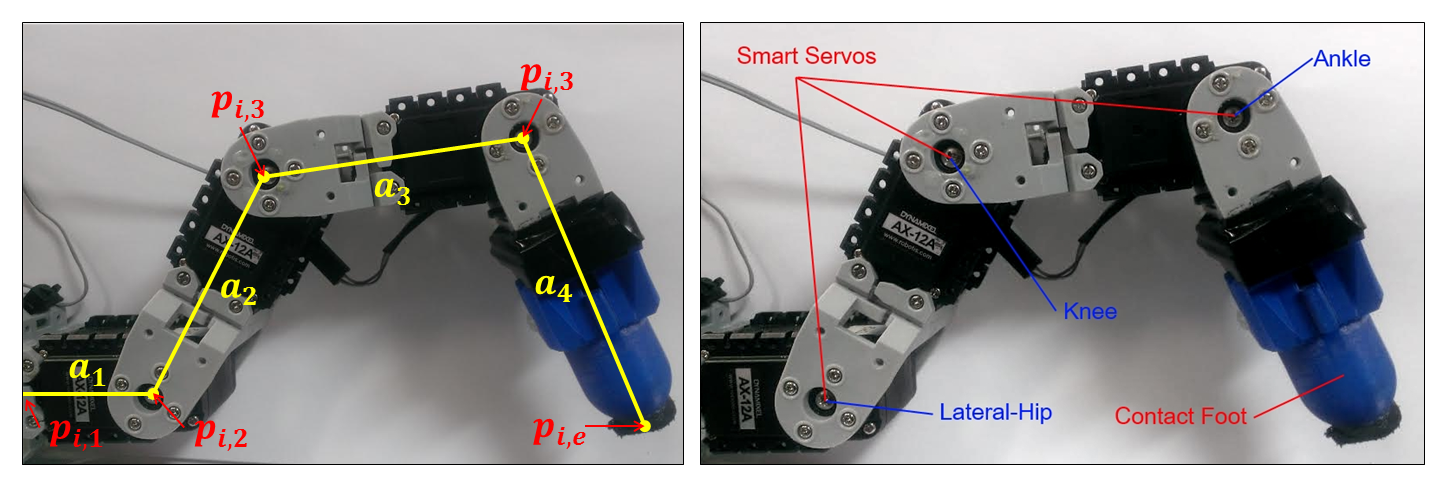
\includegraphics[width=\textwidth]{leg.png}}
				\caption{Closeup of BlueFoot's leg. \emph{(left)} shows effective link lengths and the location of defined joint positions.}
				\label{fig::leg_labeled}
			\end{figure}
				
			Each of BlueFoot's legs are identical and are comprised of four Dynamixel AX12a smart-servo actuators (see Figure \ref{fig::leg_labeled}). These actuators are connected via dedicated Dynamixel mounting brackets. Feet are attached to the ends of each leg which contain an embedded, two-state contact sensors. Each foot is designed with a spherical tip, which is rubberized to provide extra grip. The ankle joint of the platform has been added such that the platform can reconfigure its foot orientation while retaining a constant spatial position during gaiting. Additionally, this configuration allows for a considerable amount of independent body re-orientation and repositioning. This capability extends itself to the stabilization and gimbaling of vision sensors mounted on the upper body of the platform while the platform is in motion.
		
			\begin{figure}[h!]
				\centering
				\fbox{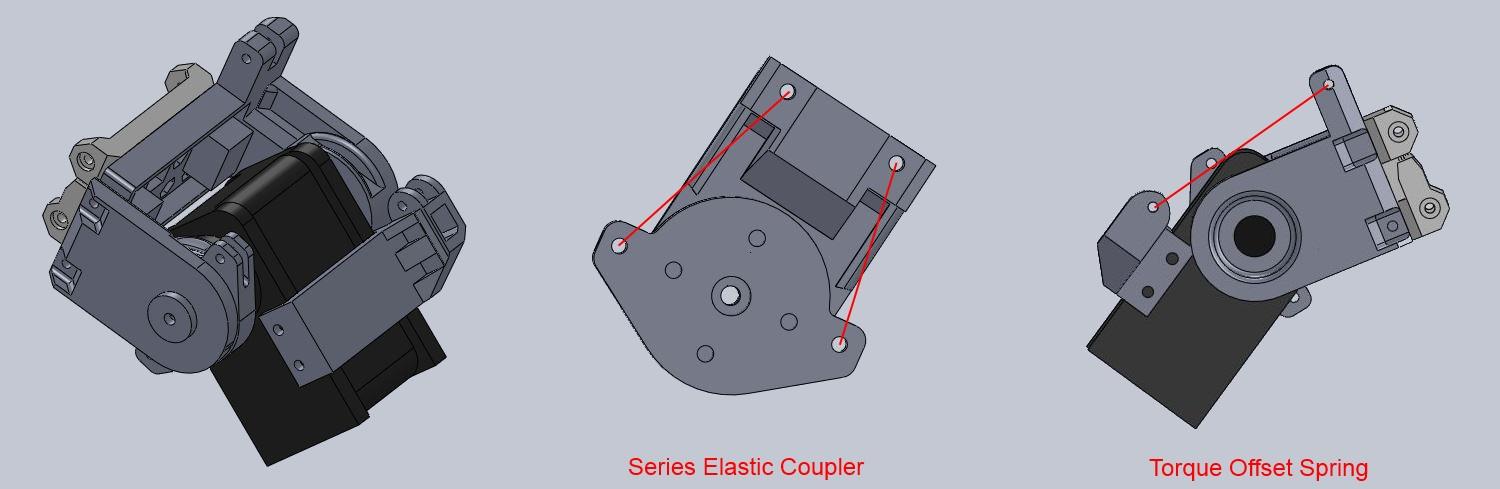
\includegraphics[width=\textwidth]{sea_full.jpg}}
				\caption{Series elastic brackets.}
				\label{fig::sea_bracket}
			\end{figure}

			Though not kept in the system's final design, some experimentation was performed with the incorporation of series elastic joints, which were designed to relieve joint impact during gaiting. Series elastic actuation was achieved by replacing bracket interfacing the first and second hip joints of each leg with an elastic-compliant mounting bracket. This bracket includes spring loaded member which was mounted to the horn of the second hip servo on each leg, as shown in Figure \ref{fig::sea_bracket} and allowed the leg to deflect a small amount at the lateral hip (second joint).

			Link lengths, $a_{1}, a_{2}, a_{3}$ and $a_{4}$; and offset from the center for the Root module to the first joint of each leg, $\nu$ are defined in Table \ref{tab::link_lens}. These parameters are identical for each leg, and are corresponded with physical leg members labeled in Figure \ref{fig::leg_labeled}.

			\begin{table}[h!]
				\centering
				\begin{tabularx}{\textwidth}{|C{0.5}|C{0.5}|} 	
					\hline
					\bf{Link} 	&	\bf{Length, m}	\\	\hline \hline
					$a_{1}$ 	&	0.06500			\\	\hline
					$a_{2}$		&	0.06500			\\ 	\hline
					$a_{3}$		&	0.06500			\\ 	\hline
					$a_{4}$		&	0.06500			\\ 	\hline
					$\nu$		&	0.09215			\\	\hline
				\end{tabularx} 
				\caption{Link and body-offset lengths for each leg.}
				\label{tab::link_lens}
			\end{table}


	\section{Computational and Sensory Hardware}
		
		\noindent
		Major payloads on-board the BlueFoot robot are as follows: 

			\begin{itemize}
				\item{Dual processor AutoPilot unit with a 12-axis inertial measurement unit}
				\item{ODROID-XU Computer}
				\item{Logitech 9000 Web-cameras}
				\item{Hokuyo-URG / Piccolo LIDAR Units (configuration dependent)}
				\item{Two-state foot contact sensors (x4)}
				\item{Dynamixel AX12a Smart Serial Servos (x16)}
				\item{XBEE Wireless radio}
			\end{itemize}

		Device selection has remained mostly consistent since the platform's inception and initial design, with the exception of computing its main computing units. The AutoPilot unit was updated from an older model, and the ODROID-XU computer replaced a Beaglebone computer for the sake of improving overall computing power.

		\subsection{Device Descriptions}
	
			\subsubsection{AutoPilot}

				A dual processor AutoPilot unit performs BlueFoot's low-level gaiting and actuator control tasks, as well as handles communications with a computer running ground-station software. Given the set of low-level sensory and motor-handling tasks it performs, this module has been named the the ``Lower Brain" (LB) of the system. The AutoPilot consists of two processing units: a TM4C and RM48 micro-controller (MCU), which operate at 80 MHz and 220 MHz, respectively. These processors communicate over a single UART line, which is used to transfer packeted data between the two processors using a unified inter-processor data transfer protocol, EXI. This protocol which will be described later in more detail. One UART of the RM48 MCU is also connected to an on-board computer, an ODROID-XU, through a USB-to-serial connection. The AutoPilot is powered via an external 12 V supply.
	
				This AutoPilot unit includes a 12-axis inertial measurement unit (IMU) which consists of two, 3-axis accelerometers; one 3-axis rate gyro; and a 3-axis magnetometer unit. This sensor is used for acquiring angular rate data of BlueFoot's trunk and estimating of trunk orientation states using an Extended Kalman Filter (EKF). 
				
			\subsubsection{ODROID-XU}

				An ODROID-XU performs many of system's high-level planning tasks, such as navigation, image processing and terrain reconstruction; and handles data data acquisition from both camera and LIDAR sensor units. Given that this unit performs mostly high-level planning tasks, it has been given the name ``Upper Brain" (UB). This computer contains a 1.6 GHz, quad-core processor with 2 Gb of RAM. The ODROID-XU can be communicated with over WiFi via a USB WiFi antenna. Currently, SSH tunneling is used to start processes on the ODROID remotely and stream data. The ODROID-XU is powered via an external 5V connection.

			\subsubsection{Logitech 9000 Web Cameras}

				Logitech 9000 web cameras have been selected for creating a stereo camera pair, as well as for use in a single camera configuration. These cameras are high-definition web cameras and have a maximum frame rate of 30 fps and a max resolution of 1280 by 720. Cameras are currently read at a the max rate of 30 fps at a more conservative resolution of 640 by 480. These settings are adequate for image processing tasks and have been chosen to reduce nominal data throughput. These cameras are interfaced with the UB (OROID-XU) over a USB connection.

			\subsubsection{Laser Distance Sensors (PLDS and Hokuyo-URG)}

				The Piccolo Laser distance sensor (PLDS), which is used in BlueFoot's stereo-camera type configuration, is a 4 meter spinning-head laser range finder. The PLDS has a resolution of a point per degree and covers a range of 360 degrees. Ranging frames (which covers a full rotation) are acquired at a rate of 5 Hz, and are dispatched over a serial connection at 115200 baud. An FTDI break-out board is used to convert the sensor's raw serial output to USB protocol so that the sensor can be interfaced with the UB unit. The PLDS is powered via and external power 5 V source, which is regulated to a 3.3 V voltage level for powering the motor which spins the laser head, and 1.8 V for internal logic. Regulation is performed by an auxiliary power circuit.

				The Hokuyo-URG Laser Distance sensor, which is used in BlueFoot's single-camera head configuration, has a a range of 5.6 metets and an angular resolution of 0.38 degrees per point (628 points per scan). This scanner covers a total angular range of 240 degrees. Ranging frames are acquired at a rate of approximately 10 Hz and dispatched directly over a USB connection at 115200 baud. The unit is powered directly over USB.

			\subsubsection{Foot Contact Sensors}

				Binary-state contact sensors are embedded in each foot. These contact sensors are essentially limit-switches which generate an active-low signal when the foot comes in contact with the ground. Each sensors is connected to ground and a GPIO pin on the TM4C MCU of the AutoPilot. A 500 $\Omega$ is added in series with the limit-switch for the purpose of pin protection.

			\subsubsection{Dynamixel AX12a Smart Serial Servos}

				BlueFoot uses 16 Dynamixel AX12a servo units (4 per leg). These servos are position-controlled and commanded over a daisy-chained, half-duplex serial bus (i.e. single wire) at a rate of 1 Mbps. These servos have a maximum holding torque of 1.618 N m and top speed of 306 degrees/s. The AX12s provide position, velocity and loading feedback, however velocity feedback is not used. Servo velocities are, instead, estimated in real time from position feedback because velocity readings provided by the AX12 is relatively noisy by comparison. 

				Commands are sent to the servos via an aggregate command packet which contains goal-position values for all servo units. Feedback is collected from each servo using individual data-request packets. Servos respond to each request with a response packet containing a corresponding feedback value. Given the number of servos in the network; communication overhead; and the one-wire communication configuration, servo updates are limited to a maximum update rate of 50 Hz over a half-duplex communication line. Gathering feedback over the half-duplex communication bus is particularly expensive because feedback requests require that the host processor wait after each dispatched for a response from each targeted servo. Moreover, each request/response cycle must finish to completion before a feedback request is made to another servo on the communication bus.

				A dedicated circuit has been designed for use with these servos which converts a full-duplex serial line to a half-duplex AX12 bus. The circuit uses a two-state tri-state buffer which is switched via a general-purpose I/O line. This switching circuit is integrated into the system's main power switching and distribution board. Each servo is powered via an fused, software-switched 12 V supply line.

			\subsubsection{XBEE Wireless Radio}

				An XBEE Wireless Radio, shown in Figure \Markup{This could be the picture from before}, is used for communication between the LB and an external computer ground-station. The radio is interfaced with the LB via 57600 baud serial connection. This radio has a range of outdoor range of 27 meters and a maximum one-way transfer-rate of 115200 bps. Transfer rates between the LB and ground station are currently being limited to 57600 bps to compensate for a lack of hardware flow-control, which is required for stable, two-way communication between two XBEE radios at maximum communication rates. However, the selected communication rate is more than adequate for transferring necessary control information to and from the system without the need for additional flow-control hardware.

				This wireless endpoint is used currently used interchangeably with the ODROID-XU's wireless WiFi radio, but will soon be retired to simplify hardware design and increase the platform's data streaming capabilities by switching to a WiFi-based line of communication. Ground station software, as well as the system's internal command-routing and networking software, is designed in such a way to easily accommodate this change.

		\subsection{Device Networking}

			\begin{figure}[h!]
				\centering
				\fbox{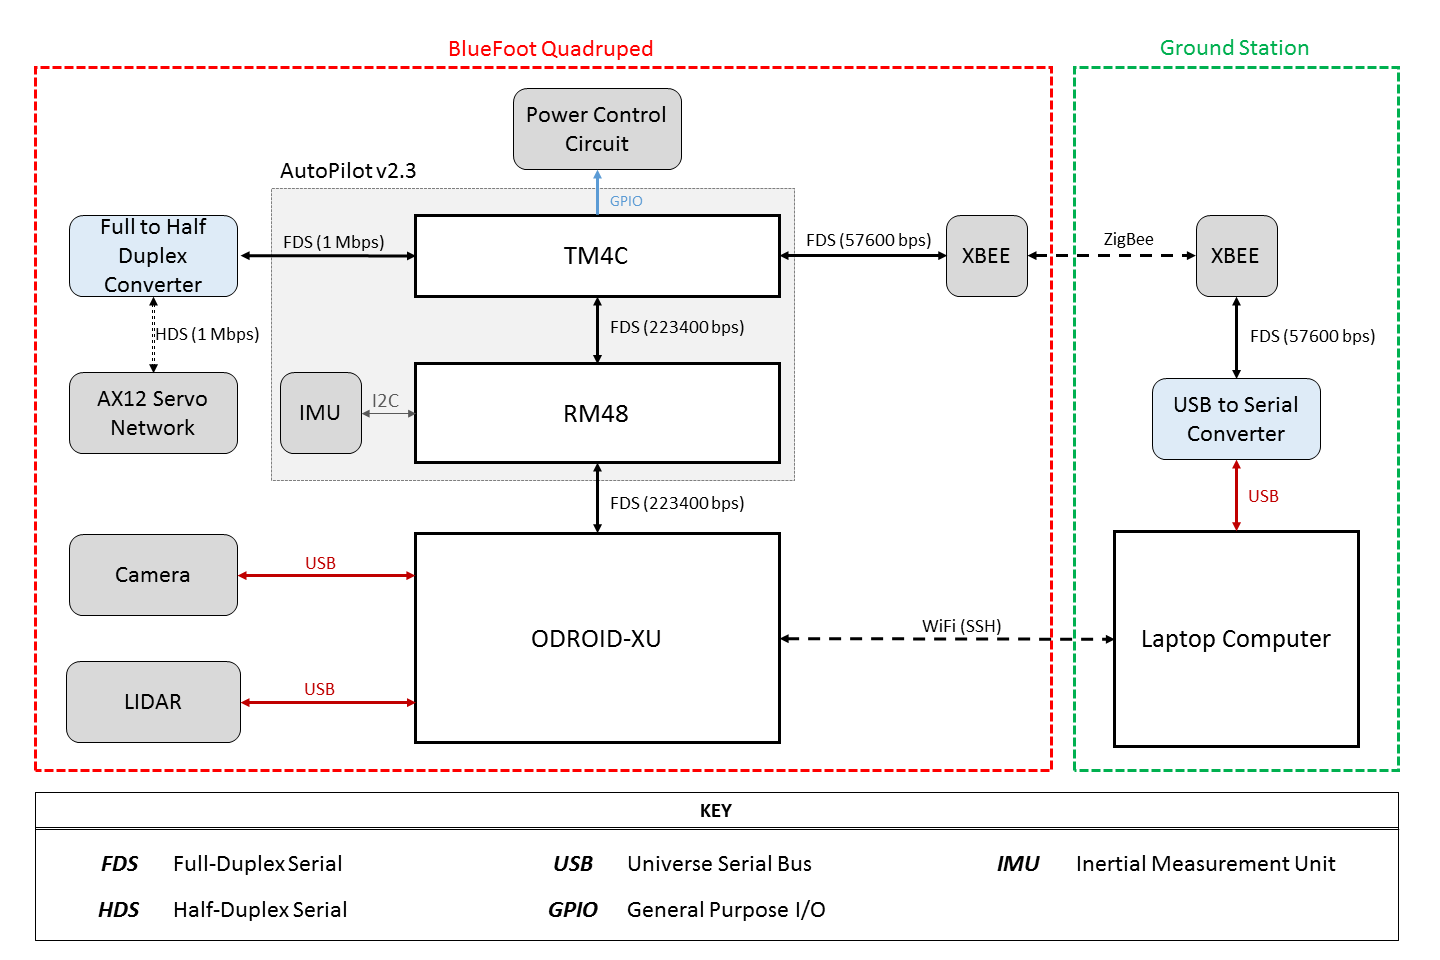
\includegraphics[width=\textwidth]{device_diagram.png}}
				\caption{BlueFoot device networking diagram.}
				\label{fig::dev_diagram}
			\end{figure}
			
			
			Figure \ref{fig::dev_diagram} depicts how each major device is connected within the system and details the communication rates ($f_{com}$) between networked devices. Accompanying specifications are detailed in Table \ref{tab::comm_port_pairs}, which summarizes all device communication pairs and their corresponding baud rates.

			\begin{table}[h!]
				\centering
				\begin{tabularx}{\textwidth}{|C{0.2}|C{0.2}||C{0.2}|C{0.2}||C{0.2}|} 	
					\hline
					\bf{Port$_A$} &	\bf{Source$_A$}	&	\bf{Port$_B$}& 	\bf{Source$_B$}	& 	\bf{$f_{com}$, kbps}\\	\hline \hline
					UART0 		&	TM4C			&	DIN/DOUT	&	XBEE$^*$		&	55.7 				\\	\hline
					UART2		&	TM4C			&	DIN+		&	AX12 Net.		&	1000				\\ 	\hline
					UART1		&	TM4C			&	LINSCI		&	RM48			&	223.4				\\ 	\hline
					SCI			&	RM48			&	USB (FTDI)	&	ODROID-XU		&	223.4				\\ 	\hline
					USB			&	ODROID-XU		&	DIN/DOUT 	&	LIDAR 			& 	115.2				\\	\hline
					USB			&	ODROID-XU		&	USB			&	Cameras	 		& 	No Spec.			\\	\hline
				\end{tabularx} 
				\caption{System communication port-pairs and corresponding data transfer rates}
				{XBEE$^*$ refers to the on-board XBEE module which communicates with the ground station.}
				\label{tab::comm_port_pairs}
			\end{table}


	\section{System Power}

		\subsection{Power Routing}

			System power routing is handled via an integrated power switching and distribution board. This board includes physical, main power switches which connects external power to two main, internal 12 volt buses for  computer power (Net-1) and motor power (Net-2), respectively. The board also regulates system input voltage to a 5 V bus for use with on-board ICs and 3.3 V bus for powering the XBEE radio. Regulated power and power the servo motors of each leg controlled via three, two-channel power-switching IC's, which are toggled using six digital I/O pins on the TM4C processor of the LB. These power-switching chips allow for software-controlled power configuration, and further, software controlled emergency power cutoff to the servo motors. System main power is supplied via four 12 V (3 cell), 2 Ah Lithium Polymer battery packs.
			%
				\begin{figure}[h!]
					\centering
					\fbox{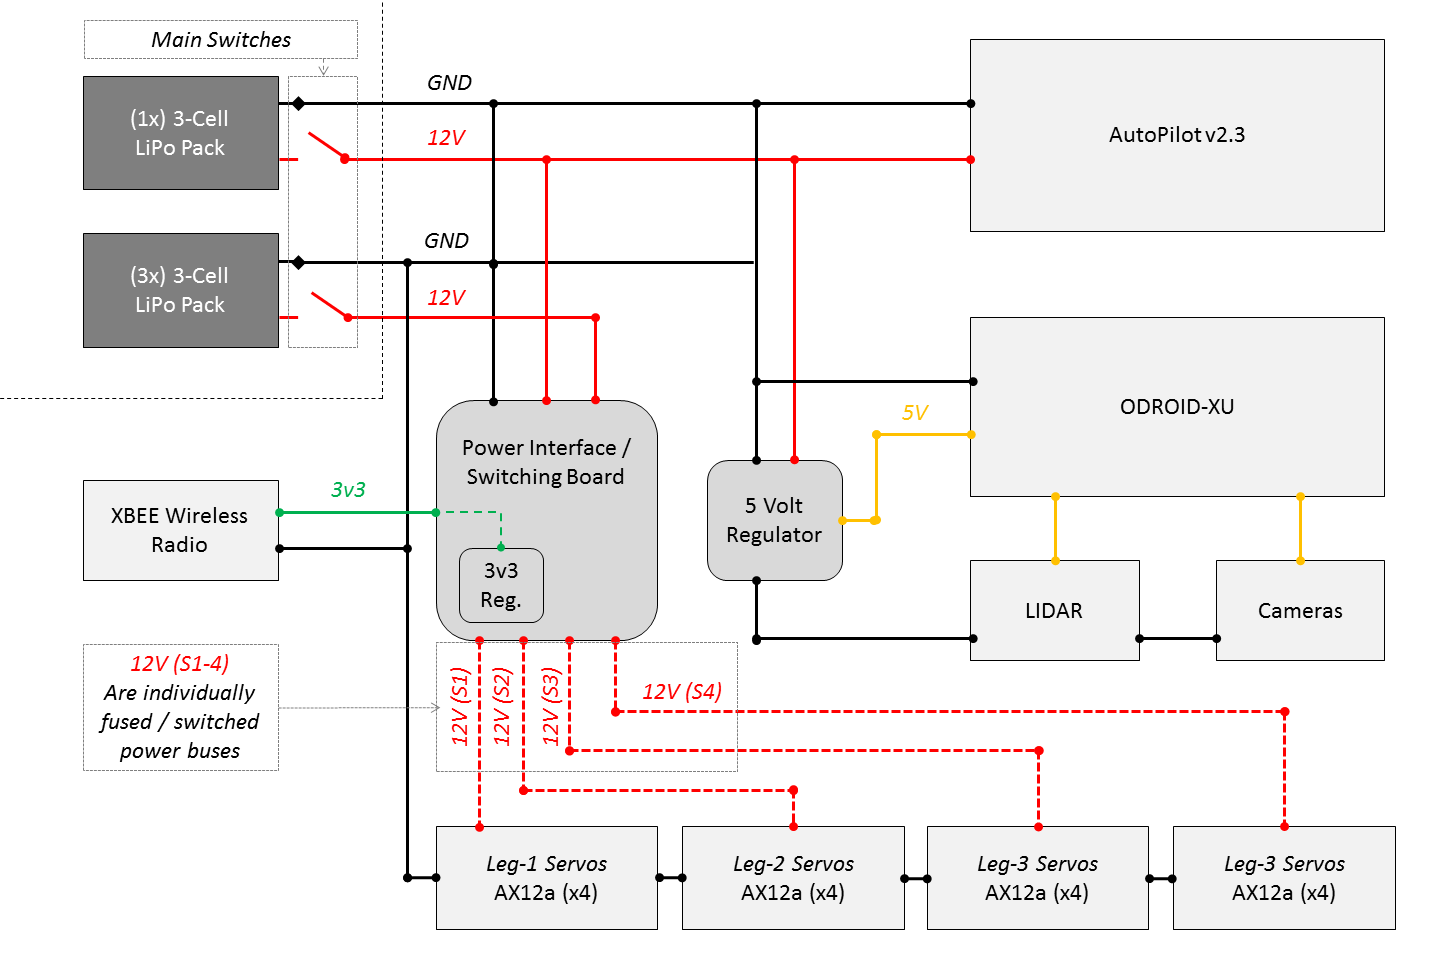
\includegraphics[width=\textwidth]{power_diagram.png}}
					\caption{BlueFoot power routing.}
					\label{fig::dev_diagram}
				\end{figure}
		
			\subsection{Energy Requirements and Runtime}

			
			The power consumptions of BlueFoot's component device's are summarized in Table \ref{tab::power_summary}, which provides the operating voltage, $V_{op}$, and nominal current draw, $I_{nom}$, of each active, on-board component. Table \ref{tab::runtime_summary} details battery specifications (output voltage and amp-hour rating) and BlueFoot's estimated run-time under nominal operating conditions.
		
		
			\begin{table}[h!]
				\centering
				\begin{tabularx}{\textwidth}{|C{0.1}|C{0.4}||C{0.25}|C{0.25}|} 
					\hline
					\textbf{Net} 	&	\textbf{Device} 		&	\textbf{$V_{op}, V$}	&	\textbf{$I_{nom}, A$}	\\	\hline\hline
					1				&	AutoPilot (RM48, TM4C) 	& 	12.0					&	0.40	 				\\	\hline
					1				&	XBEE Radio 				&	3.3						&	0.25					\\ 	\hline
					1				&	ODROID-XU 				&	5.0						&	2.0						\\ 	\hline
					1				&	Logitech-9000			&	5.0						&	0.1						\\ 	\hline
					1				&	Hokuyo-URG				&	5.0						&	0.5 					\\	\hline
					2				&	AX12a Servos (x16)		&	12.0 					&	9.6	($~$0.6 ea.)		\\	\hline
				\end{tabularx} 
				\caption{Power consumption summary by device (for single-camera configuration).}
				\label{tab::power_summary}
			\end{table}


			\begin{table}[h!]
				\centering
				\begin{tabularx}{\textwidth}{|C{0.1}|C{0.4}||C{0.25}|C{0.25}|}
					\hline
					\textbf{Net} 		&	\textbf{Battery Pack}	&	\textbf{$V_{out}, V$}			&	\textbf{Rating, $A.hr$}	\\	\hline\hline
					1				&	3S LiPo Pack (x1)		& 	12.0						&	2.0	 					\\	\hline
					2				&	3S LiPo Pack (x3)		&	12.0						&	6.0						\\ 	\hline
				\end{tabularx}

				\begin{tabularx}{\textwidth}{|C{0.5}|C{0.5}|}
					\hline
					\textbf{Total Estimated Runtime}													&	35-40 minutes			\\ 	\hline
				\end{tabularx}
				\caption{Battery power supply and estimated runtime summary.}
				\label{tab::runtime_summary}
			\end{table}
	\label{ch::software}
%%%%%%%%%%%%%%%%%%%%%%%%%%%%%%%%%%%%%%%%%%%%%%%%%%%%%%%%%%%%%%%%%%%%%%%%%%%%%%%%%%
%%% Software
%%%
%%% Section 1 : Software Architecture
%%% 
%%% Section 2 : Ground Station
%%%
%%% Section 3 : Simulator
%%%
%%%%%%%%%%%%%%%%%%%%%%%%%%%%%%%%%%%%%%%%%%%%%%%%%%%%%%%%%%%%%%%%%%%%%%%%%%%%%%%%%%
\chapter{Software}
	
	\section{System Software Architecture}
	
	BlueFoot is controlled using a multi-processor software architecture which incorporates several independent core programs. Each of these programs handles portions of system control in a cooperative fashion. Moreover, each of these processors handles specific subsets of operations essential to the macro-system. This distribution of system tasks across several core operating units allows for low-level tasks, such as actuator command and feedback handling, battery monitoring, etc., to be decoupled from more computationally heavy tasks, such as high-level planning and navigation. With task-decoupling in mind, BlueFoot's software architecture was designed such that core programs could be readily offloaded to physically separate computing modules. Each of these control modules handles their own set of assigned tasks in independent control loops. Information is forwarded from each independent processor to update the overall BlueFoot software macro-system in an asynchronous fashion. System control tasks essential to BlueFoot's overall operation are divided into four main categories, which can be summarized as follows:
		\begin{itemize}
			\item{
			\emph{Low-Level Control} : 
				power monitoring / switching, 
				actuator command handling, 
				communications routing,
				sensor data acquisition,
				script parsing and evaluation
			}
			\item{
			\emph{Locomotion Control} : 
				gait planning, 
				gait adaptation, 
				trunk pose adaptation
			}
			\item{
			\emph{High-Level Control} : 
				perception, 
				motion planning, 
				surface reconstruction, 
				navigation, 
				localization
			}
			\item{
			\emph{Human-Operator Control} : 
				joystick/keyboard commands,
				scripting commands
			}
		\end{itemize}
	Low-level and locomotion control tasks are handled, exclusively, by the \emph{Lower Brain} (LB), which designates the software collective spanning over the RM48 and TM4C processors on-board the AutoPilot. High-level control tasks are handled by the Upper Brain (UB), which is a collection of software which runs on the ODROID-XU (ODROID) module. Lastly, a human operator can interface with the system wirelessly from a personal computer running ground-station software. The ground station  communicates with the system through communication lines which enter the TM4C processor and the ODROID computer. The ground-station also interfaces with the UB over an SSH connection. This secondary wireless connection is used, mainly, for on-board data-logging configurations.

	Since this software architecture is distributed over several separate computational units, an integral part of this control architecture is an efficient, reconfigurable interprocessor communication protocol. Namely, BlueFoot utilizes data packets transfered over serial lines to update system states between processors. These data packets are formatted using an in-house designed, binary-XML protocol, called EXI. This protocol facilitates a highly customizable packeting structure for asynchronous inter-module communication and utilizes robust packet-error checking routines. This sections will detail the specifics of BlueFoot's interprocessor communication protocol, namely the composition of packets transferred between processor. 

	This section will also detail the specific software-level tasks handled by each of BlueFoot's processor; the speed at which each core software element is run (update frequency); and what data must be communicated between software elements for operation. Additionally, this section will describe the ground-station software and corresponding user-interface used to control the BlueFoot Quadruped and administer high-level commands.
	
	\subsection{System Task Allocation}

		\begin{figure}[h!]
			\centering
			\fbox{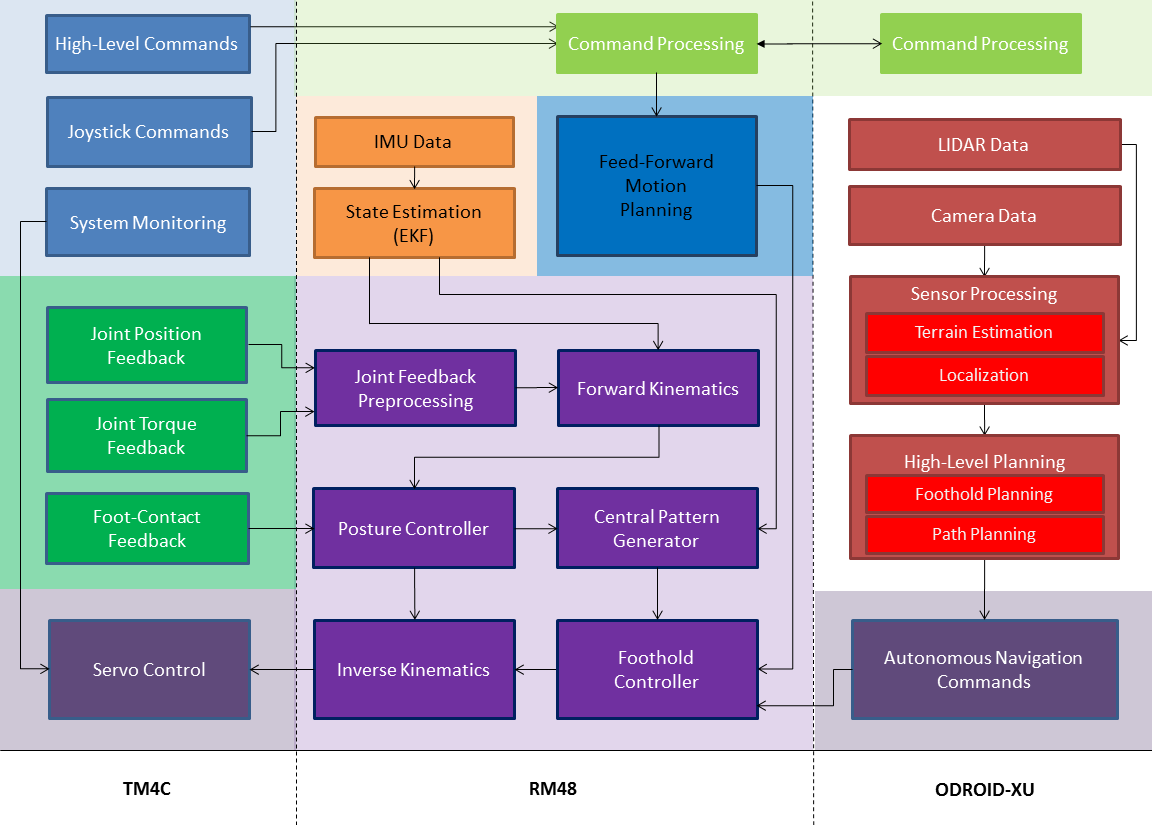
\includegraphics[width=\textwidth]{process_diagram.png}}
			\caption{BlueFoot's on-board processes/signals and their relationships.}
			\label{fig::process_diagram}
		\end{figure}

		Figure \ref{fig::process_diagram} depicts how core software and associated control elements are related within the BlueFoot software macro-system. This section will detail a general description of the tasks carried out by each major software module implemented on the BlueFoot quadruped.

		\subsubsection{TM4C (Lower Brain)}

			As previously mentioned, the TM4C processor on-board the AutoPilot module is responsible for \emph{Low-Level} tasks and can be viewed a safety/communications routing co-processor within the overall system. Within its main program loop, the TM4C polls the system's main battery voltage via ADC interface routines; handles transmit and receive (packet decoding) routines between the ground-station and the RM48 system nodes; and handles command dispatching and feedback polling with the system's 16 servo actuators. The TM4C is directly interfaced with two dual-channel power switching IC's and is used to control power supply to each leg by toggling general purpose IO pins in software. The state of these pins is administered as part of a periodic packet command/update packet sent from the ground-station. Since the TM4C has this control over the system's actuators (which consume most of the system's power) and battery monitoring capabilities, it runs a safety routine which is responsible for halting motor activity and/or cutting system power on low-battery or power-fault conditions, as well as during unexpected breaks in communication with the ground-station.

			As previously mentioned, the TM4C handles communication routing between system processing modules; as well as with controllers on-board each smart-servo. Administering servo commands and collection servo feedback it the TM4C's highest priority task. This process, which involves both commanding and requesting feedback from each servo, is relatively expensive  and limits the TM4C's loop frequency to roughly 50 Hz. Thus, it is particularly important that this task is offloaded to this processor, as its other safety and communication-related tasks are much less expensive, by comparison, and allow the servo actuators to be updated quickly as possible without encumbering other system control operations.


		\subsubsection{RM48 (Lower Brain)}

			The RM48 is responsible for several \emph{Low-Level} tasks, including IMU polling and handling communication with the TM4C and ODROID-XU. Each collected IMU sample is passed along to an extended Kalman Filter routine, which generates a trunk orientation estimate, $\hat{\theta}_{b}$, in the world frame, $O_{0}$. 

			The RM48's primary function is to carry out motion control and gait-planning tasks. To achieve this, the RM48 handles a state machine which switches between planned motion execution and trajectory control; and gait control via a Central Pattern Generator (CPG) based gaiting controller, which will be discussed in more detail in Chapter~\ref{ch::gait_control}. Additional functions for body and posture (position and orientation) control, including trunk leveling procedures, and gait-stabilization are run in tandem with the aforementioned gait-control task.

			Motion and gait controls, which are performed in the robot task-space, are converted into joint-space reference angles, $q^{r}$, via an inverse kinematics (IK) routine. The IK routine is executed at all times when the legs are engaged for the purpose of issuing servo position commands, given desired task-space configurations for body and feet positions, which will be more formally defined in Chapter~\ref{ch::system_modeling}. The RM48 also maintains BlueFoot's forward kinematic model (specifically, foot position relative to the trunk), which relies on an EKF-generated trunk orientation estimate, $\hat{\theta}_{b}$, and joint position feedback, $q$. BlueFoot's inverse and forward kinematics models will be detailed in Chapter~\ref{ch::system_modeling}. The RM48 runs its full control loop at approximatively 100 Hz (twice the speed of the TM4C control loop) to facilitate higher integration stability when updating gait related controller dynamics, dynamic motion controls, task-space reference trajectories.

			Lastly, the RM48 handles an on-board scripting engine (based on the MIT Squirrel scripting language), which interprets lexical commands. This scripting engine is capable of handling a large number of high-level commands and is complex enough to handle function and class definitions in real time \cite{Squirrel_website}. The scripting engine currently being used to evaluate BlueFoot's core user command set, ranging from simple state toggling and parameter modification, to the prescription of user-specified way-points for navigation, among other high-level command items. Scripting commands are passed from the ground station (via terminal) and routed through the TM4C to the RM48, where they are finally evaluated.

		\subsubsection{ODROID-XU (Upper Brain)}

			The ODROID-XU runs software upon a Debian (Linux) operating system distribution ``Jessie." The use of an Linux operating system extends itself to a number of programmatic conveniences, such as to ability to run several tasks in parallel threads. Inbuilt USB drivers are used in functions which are used to acquire data from USB-interfaced vision sensors. Namely, the ORDOID runs sensor handling elements used for acquiring and buffering camera images and controlling camera frame-rate control; as well as LIDAR scan frames. The ORIOID uses these sensor inputs, in conjunction with orientation estimates and inertial data passed from the RM48 to perform several navigation-related tasks (\EG potential fields, mapping, localization, terrain-reconstruction). These tasks will be described in more detail in Chapter~\ref{ch::navigation}.

			The ODROID utilizes 2D-LIDAR scans (frames) and trunk-pose estimates to form organized 3D point clouds. These point-clouds are further processed to reconstruct 3D terrain surfaces and height-maps, which are then used for step-planning. LIDAR frames are utilized in potential fields-based navigation tasks. These navigation modes also incorporate camera data for the purpose of goal-targeting (where the goal is typically an object of particular shape or color). Image processing and image feature detection is run as a separate process on the ODROID, which is incorporated with the aforementioned processed sensor data to produce a set of forward and turning velocity commands, $v^{r}$ and $\omega^{r}$, respectively; as well as foot-hold positions generated from step-planning algorithms. In particular, the open-source libraries OpenCV (Open Computer Vision Library), OpenPCL (Open Point-Cloud Library), and Boost are heavily used in the software developed to carry out the aforementioned tasks \cite{opencv_library,openpcl_library,boost_website}. Software written for this platform was generated using a mixture of C++ and Python.

			As previously mentioned, the ODROID can handle a limited set user-command on its own, which are administered directly to the ODROID from an SSH terminal on the ground-station computer. These commands include core-program start-ups and data-logging configurators. Essentially, the ODROID's software core is designed as a completely independent software module which replaces the roll a human director, as it handles the bulk of the systems high-level planning and navigation tasks. Moreover, if the ODROID is removed from the BlueFoot system, the system can still be operated via remote-control heading commands provided from human operator (\IE ground-station joystick control).
		
		\subsection{Inter-processor Communication}

			\begin{figure}[h!]
				\centering
				\fbox{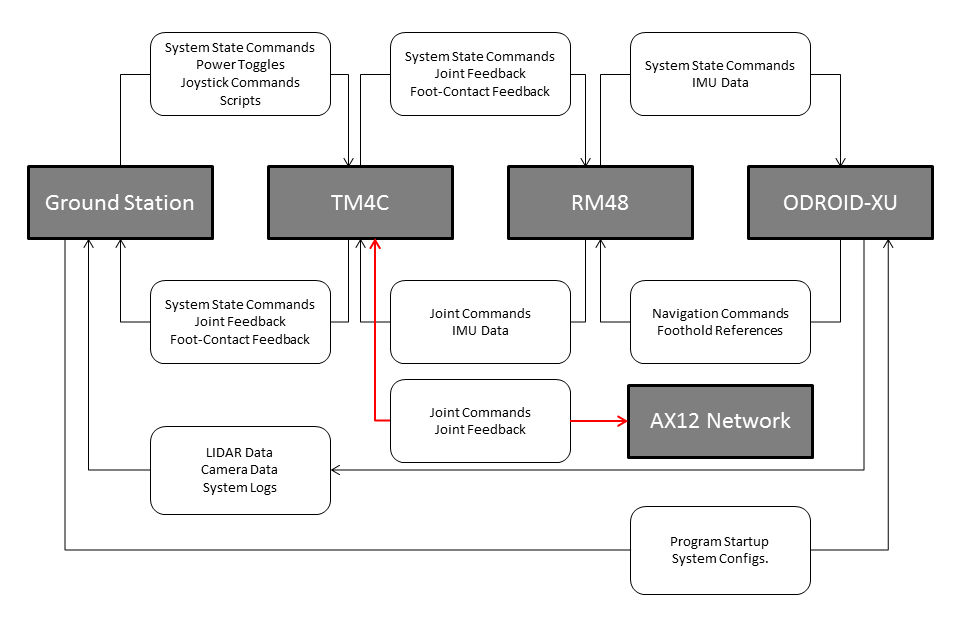
\includegraphics[width=\textwidth]{comm_flow.png}}
				\caption{Communication flow between processors on the BlueFoot Platform.}
				\label{fig::comm_flow}
			\end{figure}

			This section will detail the contents of the data packets transfered between processors, which is summarized in Figure \ref{fig::comm_flow}. System directives, generated by a human operator who interacts with the robot via a graphical user interface and/or joystick controllers, are generated from a ground-station computer. Packets (without padding) sent from the ground station to the BlueFoot robot (TM4C) are composed as shown in Table \ref{tab::gs_to_tm4c_packet}:
			\begin{table}[h!]
				\centering
				\begin{tabularx}{\textwidth}{|C{0.2}|C{0.2}|C{0.2}|C{0.2}|C{0.2}|} 	
					\hline
					\emph{32-bits} 	& \emph{8-bits} 		& \emph{8-bits} 	&\emph{16-bits} 	& \emph{16-bits} 	\\\hline
					HEADER 		& Master-Tog.		& Power-Tog.	& Unused		& Network Info 	\\\hline
					\emph{Variable} 	& 		 		& 			&			& 			\\\hline
					Scripts 		& 				& 			& 			&			\\\hline
				\end{tabularx} 
				\caption{Structure of the packets sent from Ground-Station to TM4C.}
				\label{tab::gs_to_tm4c_packet}
			\end{table}
			
			Every packet issued using the EXI protocol has a 4-byte (32-bit) header. As part of the internal system protocol, every packet sent between system nodes contains a ``Master Status Vector", which is comprised of a fixed length, 7-byte sequence of essential system information and control items. The ``Master Toggles" section (first 8-bits after header) enumerates major systems states, including \emph{On-line, Standby, Off-line} and \emph{Suspended} system state designations. The next 8-bits are used to toggle on-board power, namely the power supplied to each leg. The remaining 32-bits are used for specifying battery voltage (8-bits), power-fault states (8-bits), generic binary feedback toggles (8-bits), and system networking information (16-bits). The last section of this packet contains scripting commands, which can be of varying lengths. For example, forward velocity and turning rate commands (gathered form a joy-stick controller) are administered in the form of scripted commands.

			Packets sent from the TM4C to the Ground-station contain status items generated on board the robot, and appear as shown in Table \ref{tab::tm4c_to_gs_packet}:
			\begin{table}[h!]
				\centering
				\begin{tabularx}{\textwidth}{|C{0.2}|C{0.2}|C{0.2}|C{0.2}|C{0.2}|} 	
					\hline
					\emph{32-bits} 	& \emph{8-bits} 		& \emph{8-bits} 	& \emph{8-bits} 	& \emph{16-bits} 	\\\hline
					HEADER 		& Master-Tog.		& Unused		& Foot-Contacts	& Network Info 	\\\hline\hline
					\emph{2048-bits} 	& 				&			&  			& 		 	\\\hline
					Joint Pos. FB		& 				& 			& 			& 			\\\hline
				\end{tabularx} 
				\caption{Structure of the packets sent from the TM4C to the Ground-Station.}
				\label{tab::tm4c_to_gs_packet}
			\end{table}
			The \emph{Joint Pos. FB} (joint position feedback) element is composed of 16 2-byte sequences corresponding to the joint positions of read-back by each actuator. To avoid redundancy, the structure of the packets communicated from the TM4C to the RM48 and vice-versa will not be depicted explicitly. Like all system packets, these packets contain a 7-byte master status vector with only the \emph{Master-Toggle} and \emph{Network Info} fields populated. The TM4C sends the same joint feedback information to the RM48 as it does the Ground Station. For packets sent from the TM4C to the RM48, this field is replaced with corresponding joint-position commands for each of the 16 servo actuators. This field is also 2048 bits in length.

			Packets sent from the RM48 to the ODROID contain additional dynamical-state fields for use in planning on the ODROID. State information is sent in the form a vectors with 32-bit, single precision floating-point elements. This set of information includes trunk a orientation estimation, angular rate, and global position (generated from open-loop command integration), each of which are represented as 3-element vector; and foot-position estimates (four, 3-element vectors.) generated. These packets have a structure which is depicted in Table \ref{tab::rm48_to_odroid}.
%
			\begin{table}[h!]
				\centering
				\begin{tabularx}{\textwidth}{|C{0.2}|C{0.2}|C{0.2}|C{0.2}|C{0.2}|} 	
					\hline
					\emph{32-bits} 	& \emph{8-bits} 		& \emph{8-bits} 	& \emph{8-bits} 	& \emph{16-bits} 	\\\hline
					HEADER 		& Master-Tog.		& Unused		& Foot-Contacts	& Network Info 	\\\hline\hline
					\emph{96-bits} 	& \emph{96-bits}		& \emph{328-bits}	&\emph{328-bits}  	& 		 	\\\hline
					Orientation		& Angular Rate		& Trunk Pos.		& Foot Positions	& 			\\\hline
				\end{tabularx} 
				\caption{Structure of the packets sent from the RM48 to the ODROID.}
				\label{tab::rm48_to_odroid}
			\end{table}
		Packets sent form the ODROID to the RM48 contain command items, such as forward velocity, turning rate and trunk-pose commands, as well as foothold-references and corrected global trunk position estimates. These packets are constructed as shown in Table \ref{tab::odroid_to_rm48} :
%
			\begin{table}[h!]
				\centering
				\begin{tabularx}{\textwidth}{|C{0.2}|C{0.2}|C{0.2}|C{0.2}|C{0.2}|} 	
					\hline
					\emph{32-bits} 	& \emph{8-bits} 		& \emph{8-bits} 	& \emph{8-bits} 	& \emph{16-bits} 	\\\hline
					HEADER 		& Master-Tog.		& Unused		& Unused		& Network Info 	\\\hline\hline
					\emph{32-bits} 	& \emph{32-bits}		& \emph{96-bits}	&\emph{328-bits}  	& \emph{96-bits} 	\\\hline
					Velocity		& Turning Rate		& Trunk Pose		& Footholds.	& Trunk Pos.		\\\hline
				\end{tabularx} 
				\caption{Structure of the packets sent from the ODROID to the RM48.}
				\label{tab::odroid_to_rm48}
			\end{table}

	\section{Ground Station}
		
		%\begin{figure}[h!]
		%	\centering
		%	\fbox{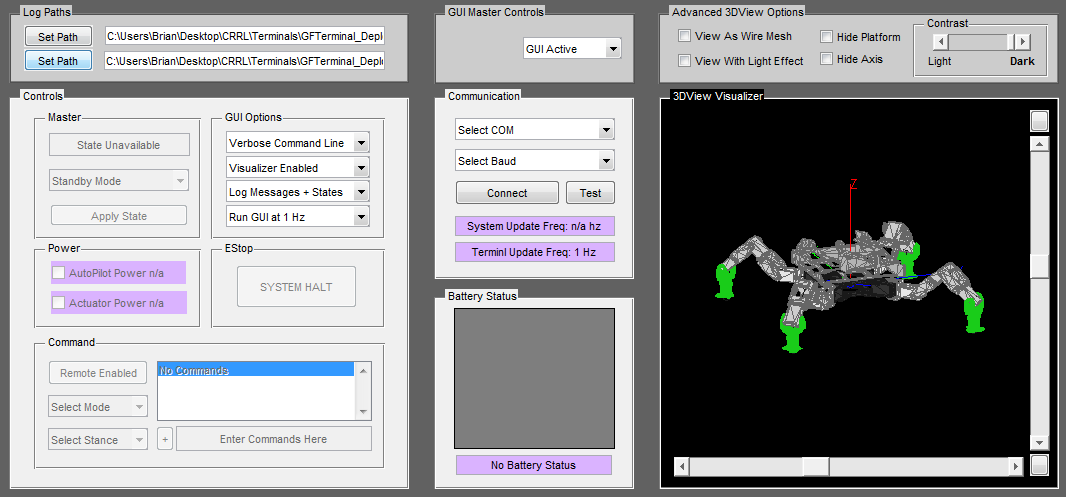
\includegraphics[width=\textwidth]{terminal.png}}
		%	\caption{BlueFoot ground-station GUI}
		%	\label{fig::comm_flow}
		%\end{figure}
		%\begin{figure}[h!]
		%	\centering
		%	%\fbox{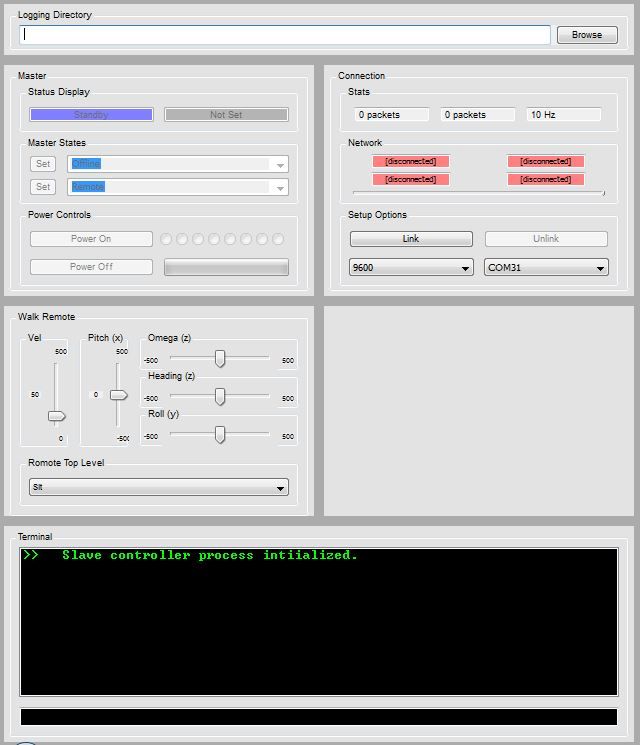
\includegraphics[width=\textwidth]{wxTerminal.jpg}}
		%	\caption{Version 2 of the BlueFoot ground-station GUI, implemented with \emph{wxWidgets}}
		%	\label{fig::comm_flow}
		%\end{figure}s
	Ground-station software used for controlling the BlueFoot platform is generated in C++ using an open-source graphical user interface design library called \emph{wxWidgets} \cite{WX_Website}. \emph{wxWidgets} is used, primarily, for the ground-station's front-end design. Namely, the ground-station code is designed such that that its UI design is reconfigurable via an XML-based design specification file. Furthermore, this allows for UI reconfigurations without the need to change internal, back-end processes. In terms of the GUI back-end, \emph{wxWidgets} handles general UI signal processing, and allows for easy registration of user callbacks on events such as button presses. Additionally, \emph{wxWidgets} provides an interface for collective joystick inputs, which are interpreted and sent to the BlueFoot as remote-control commands. \emph{Boost}, a C++ utility library, is utilized to provide socket and serial-port IO handling. This library is particularly important handling serial-IO ports on the ground station computer, which are used in communicating with the robot over a wireless radio connection.

	The ground station is composed of several main UI sections provide interfaces for administering system master-state, operating-state and power toggling; providing system commands; and scripting. Basic system state controls are used to periodically populate a fixed-structure, robot-command packet, shown in Table \ref{tab::gs_to_tm4c_packet}. This packet is used to refresh the robot operating state and manual navigation commands. Updates from the ground-station are sent to the platform rate of 25 Hz using the an XBEE radio module. BlueFoot replies to each ground-station update with a packet of internal configurations, as shown in Table \ref{tab::tm4c_to_gs_packet}, which is then used to ensure that system updates and commands have been received and that the system is live.

	Namely, BlueFoot sends the following particles of system information back to he ground-station: 
	\begin{itemize}
		\item battery voltage levels 
		\item power fault conditions 
		\item foot contact feedback
		\item and joint position feedback. 
	\end{itemize}
	This data is used to update several key portions of the UI. Firstly, battery levels are used to update a battery meter, which indicates the current system voltage level. Additionally, a dynamic text box displays the system's power-fault state to the user. Joint position commands are used to update a visualization of the robot in real time. The foot-color of the visualized BlueFoot robot changes from blue to red to represent foot-contact conditions. Joint positions, foot-contact states and battery levels are time-stamped and automatically logged during each ground-station session. 


	%%%%%%%%%%%%%%%%%%%%%%%%%%%%%%%%%%%%%%%%%%%%%%%%%%%%%%%%%%%%%%%%%%%%%%%%%%%%%%%%%%
%%% Control
%%%
%%% NEED TO FIX NOTATIONS
%%%
%%%%%%%%%%%%%%%%%%%%%%%%%%%%%%%%%%%%%%%%%%%%%%%%%%%%%%%%%%%%%%%%%%%%%%%%%%%%%%%%%%
\chapter{System Modeling}
	\label{ch::system_modeling}

	%Analysis and control of the BlueFoot quadruped requires the utilization of both kinematic and dynamical system models.
	
	\section{Kinematic Model}
		\label{sec::system_kinematics}

		The kinematic model of the BlueFoot platform is paramount for trajectory planning, localization, and adaptation in the robot task-space. In particular, inverse position and velocity solutions are used to prescribe joint-space commands from particular foot trajectories planned in the world coordinate frame. Additionally, BlueFoot's forward kinematic model is utilized to estimate the position of each foot using the position and orientation of the trunk; and joint position feedback. This section will describe BlueFoot's forward and inverse kinematic models, as well as how these models are used in motion planning and control tasks.

		\subsection{Forward Position Kinematics}
			\label{ch::system_modeling_pos_kin}

			To formulate the kinematics model, a set of coordinate systems have been defined and are described by Figure~\ref{fig::coordinate_frames}. Note that the frame $O_{0}$ represents the world coordinate frame; and $O_{b}$ is the coordinate frame, centered at  ${p}_{b}$ attached to the platform and is always aligned with $O_{0}$. $O_{b}$ represents a body frame rigidly attached to the center of the trunk. The orientation and position of the trunk are defined by vectors of $\theta_{b}\InRe{3}$ and ${p}_{b}\InRe{3}$, which relate the frame $O_{b}$ to the world frame $O_{0}$. Coordinate frames $O_{i,0}$ are attached to the first joint of each \Ith leg.
%
				\begin{figure}[h!]
					\centering
					\fbox{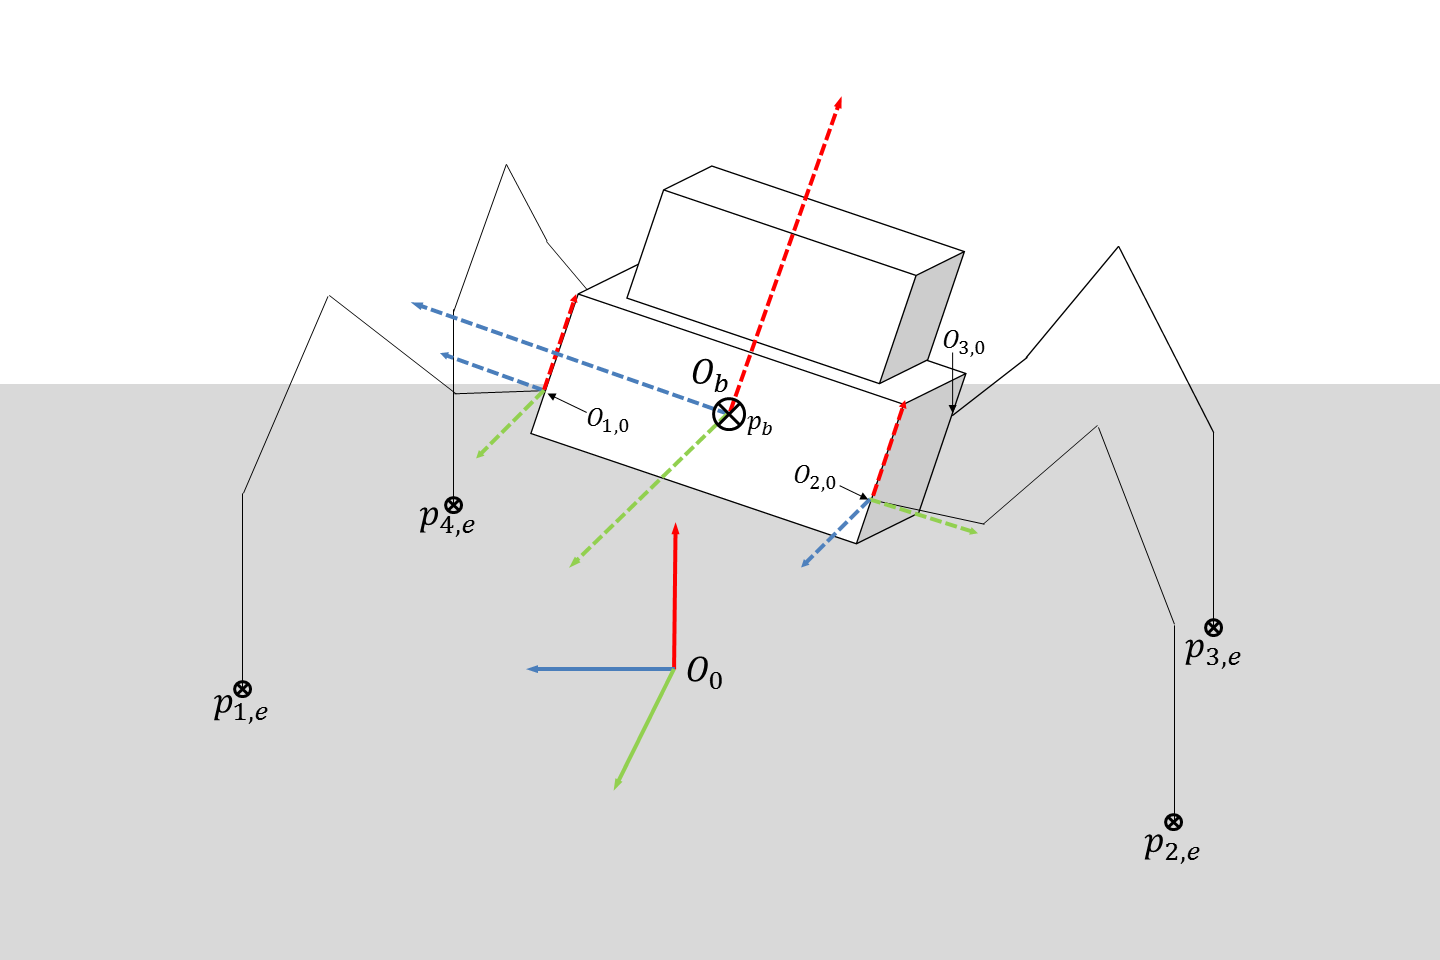
\includegraphics[width=1.00\textwidth]{coordinate_frames.png}}
					\caption{A visualization of BlueFoot's coordinate frame configuration.}
					\label{fig::coordinate_frames}
				\end{figure}
%
			The \Jth joint position of each \Ith leg is represented  by the points ${p}_{i,j}$ in the frame $O_{0}$. These spatial locations are generated from a combination of the body orientation, $\theta_{b}$, and joint positions for each \Ith leg, $q_{i} = [q_{i,1}, q_{i,2}, q_{i,3}, q_{i,4}]^T$. $q_{i,1}$ represents the position of the hip-joint (joint closest to the center platform), which rotates in the direction of the transverse body plane. The joint variables $q_{i,2}, q_{i,3}$ and $q_{i,4}$ represent the lateral-hip, knee and ankle joint rotations, respectively.

			The coordinate transformation between world coordinate frame, $O_{0}$, and the zeroth Denavit-Hartenberg (DH) coordinate frame of leg \emph{i}, $O_{i,0}$ (located at the origin of joint-1), is given by
				\begin{equation}
					H_{0}^{i,0} = \left[ 
					\begin{array}{c|c}
						R_{zyx}(\theta_{b}) R_{z}(\sigma_{i})	&R_{zyx}(\theta_{b}) \nu + {p}_{b} 	\\ \hline
						0										&	1											\\
					\end{array} 
					\right]
					\label{eq::world_to_dh}
				\end{equation}
			where $\sigma_{i} \equiv \frac{\pi}{2}(i-1) + \frac{\pi}{4} $ and $\nu \equiv  R_{z}(\sigma_{i}) \beta$ with $\beta$ defining an offset from $O_{b}$ to where the first joint of each leg is attached to the body. $R_{zyx}$ represents a rotation associated with the pitch (x-axis), roll (y-axis), and yaw (z-axis) angles of the main body about the platform frame, $\theta_{b}$. $R_{z}$ represents a rotation about the (z-axis) of the frame $O_{b}$. 

			A transformation from the zeroth DH frame of the to the $(j+1)^{th}$ joint of leg \emph{i} is described, in general, by
				\begin{equation}
					H^{i,0}_{i,j} =
					\left[ 
					\begin{array}{c|c}
						R^{i,0}_{i,j} 	&	{p}^{i,0}_{i,j} 	\\ \hline
						0			&	1				\\
					\end{array} 
					\right].
				\end{equation}

			The kinematics of each leg are identical. Thus, the transformations $H^{i,0}_{i,j}$ are of the same form and are derived by the DH parameters given by Table \ref{tab::dh_params}. Actual values for the link lengths $a_{1-4}$ and body-offset, $\nu$, are provided in Table \ref{tab::link_lens}.


			\begin{table}[h]
				\centering
				\begin{tabularx}{150mm}{|C{0.2}|C{0.2}|C{0.2}|C{0.2}|C{0.2}|} \hline
					\textbf{Link}	&\textbf{$a_i$} &	\textbf{$\alpha_i$}	&	\textbf{$d_i$}	&	\textbf{$\theta_i$} \\ \hline \hline
					1				&	$a_{1}$		&	$\pi/2$				&	0				&	$q_{i,1}^*$			\\ \hline
					2				&	$a_{2}$		&	0					&	0				&	$q_{i,2}^*$			\\ \hline
					3				&	$a_{3}$		&	0					&	0				&	$q_{i,3}^*$			\\ \hline
					4 				&	$a_{4}$		&	0					&	0				&	$q_{i,4}^*$			\\ \hline
				\end{tabularx}
				\caption{DH parameters for all legs.}
				\label{tab::dh_params}
			\end{table}
			

			Using these DH parameters, the transformations $H^{i,0}_{i,1}$, $H^{i,0}_{i,2}$, $H^{i,0}_{i,3}$, and $H^{i,0}_{i,4}$ can be computed explicitly as follows:
				%% Manipulator Base to Frame 1 %%
				\begin{equation} 
					H^{i,0}_{i,1} =\left[ 
					\begin{array}{ccc|c}
						c_{1,i} 	&  		0	& 	s_{1,i}		&		c_{1,i} a_{1,i}	\\
						s_{1,i} 	&  		0	& 	-c_{1,i}	&		s_{1,i} a_{1,i}	\\
						0 			&  		1	& 	0			&		0 				\\ \hline
						0 			&  		0	& 	0			&		1 				\\
					\end{array} 
					\right]
					\label{eq::transform1}
				\end{equation}
				%% Manipulator Base to Frame 2 %%
				\begin{equation}
					H^{i,0}_{i,2} =\left[ 
					\begin{array}{ccc|c}
						c_{1,i} c_{2,i}	&  		-c_{1,i} s_{2,i}	& 		s_{1,i}		&	c_{1,i}( a_{1,i} + a_2 c_{2,i} )\\
						s_{1,i} c_{2,i}	&  		-s_{1,i} s_{2,i}	& 		-c_{1,i}	&	s_{1,i}( a_{1,i} + a_2 c_{2,i} )\\
						s_{2,i} 		&  		c_{2,i}			 	& 		0			&	a_2 s_{2,i} 					\\ \hline
						0 			&  		0			 		& 		0			&	1 								\\
					\end{array} 
					\right]
					\label{eq::transform2}
				\end{equation}
				%% Manipulator Base to Frame 3 %%
				\begin{equation}
					H^{i,0}_{i,3} =\left[ 
					\begin{array}{ccc|c}
						c_{1,i} c_{23,i}	&  		-c_{1,i} s_{23,i}	& 		s_{1,i}		&		c_{1,i}( a_{1,i} + a_2 c_{2,i} + a_3 c_{23,i} )	\\
						s_{1,i} c_{23,i}	&  		-s_{1,i} s_{23,i}	& 		-c_{1,i}	&		s_{1,i}( a_{1,i} + a_2 c_{2,i} + a_3 c_{23,i} )	\\
						s_{23,i} 		&  		c_{23,i}			& 		0			&		a_2 s_{2,i} + a_{3,i} s_{23,i}			\\ \hline
						0 			&  		0					& 		0			&		1 										\\
					\end{array} 
					\right]
					\label{eq::transform3}
				\end{equation}
				%% Manipulator Base to Frame 4 %%
				\begin{equation}
					H^{i,0}_{i,4} =\left[ 
					\begin{array}{ccc|c}
						c_{1,i} c_{234,i}	&  		-c_{1,i} s_{234,i}	& 		s_{1,i}		&		c_{1,i}( a_{1,i} + a_2 c_{2,i} + a_3 c_{23,i} + a_4 c_{234,i} )		\\
						s_{1,i} c_{234,i}	&  		-s_{1,i} s_{234,i}	& 		-c_{1,i}	&		s_{1,i}( a_{1,i} + a_2 c_{2,i} + a_3 c_{23,i} + a_4 c_{234,i} )		\\
						s_{234,i} 		&  		c_{234,i}		& 		0			&		a_2 s_{2,i} + a_3 s_{23,i} + a_4 s_{234,i}					\\ \hline
						0 			& 		0			& 		0			&		1 															\\
					\end{array} 
					\right]
					\label{eq::transform4}
				\end{equation}
			A summary of the abbreviations used to represent trigonometric terms found in \ref{eq::transform1}-\ref{eq::transform4} are summarized in.

			The position of joint 1 of leg \emph{i} in $O_{0}$, ${p}_{i,1}$ may now be computed with respect to frame $O_{0}$ by:
				\begin{equation}
					{p}_{i,1} \equiv E_{p} H_{0}^{i,0} e_{p}.
					\label{eq::world_joint1_position}
				\end{equation}
			where
				\begin{eqnarray}
					E_{p} = [I_{3\times3},0_{3\times1}]	\nonumber 	\\
					e_{p} = [0_{1\times3},1]^T.			\nonumber 	
				\end{eqnarray}
			The position of joints 2-4 of leg \emph{i}, may now be computed with respect to frame $O_{0}$ by:
				\begin{equation}
					{p}_{i,j} \equiv E_{p} H_{0}^{i,0} {H}^{i,0}_{i,(j-1)} e_{p}. \Sep \forall \Sep j\in\{2,3,4\}
					\label{eq::world_joint_positions}
				\end{equation}
			Finally, the position of the end-effector (foot) of \Ith leg. ${p}_{i,e}$, is achieved as follows:
				\begin{equation}
					{p}_{i,e} \equiv E_{p} H_{0}^{i,0} {H}^{i,0}_{i,4} e_{p}.
					\label{eq::world_feet_positions}
				\end{equation}
			As a previously mentioned, BlueFoot's forward kinematic solution is used most prevalently in the estimating the position of each foot. Given estimates for body position and orientation, $\hat{p}_{b}$ and $\hat{\theta}_{b}$, a foot position estimate is explicitly define as a random variable:
				\begin{equation}
					\hat{p}_{i,e} = {p}_{i,e} + \Delta {p}_{i,e}
					\label{eq::foot_position_esitmate}
				\end{equation}
			where $\Delta {p}_{i,e}$ is a random error which arises from variations due to noise in sensed joint positions, as well as error in the estimates $\hat{p}_{b}$ and $\hat{\theta}_{b}$.


			\subsubsection{A Note about foot localization in the robot-relative frame, $O_{b^{'}}$}

			Using the previously defined forward kinematics model and the relationships defined in \ref{eq::world_joint_positions} and \ref{eq::world_feet_positions}, the position of each joint and foot can be computed assuming the $p_{b}$ and $\theta_{b}$ are known (or can be estimated) in the frame $O_{0}$. Provided inertial feedback, trunk orientation, $\theta_{b}$, can be estimated by the use of an Extended Kalman Filter (EKF). $p_{b}$, however, requires more sophisticated localization measures, such as a Simultaneous Localization and Mapping (SLAM) scheme or absolute positioning via overhead camera or GPS. In lieu of an implementation for such a localization routine, it is convenient to generate foot positions estimate in a \emph{robot-relative} frame, $O_{b^{'}}$. This frame is not rigidly attached to the robot but moves along with the robot in $O_{0}$ according to the commanded translational velocity, $v^{r}$, and turning rate. $\omega^{r}$, administered to navigate the system. These values will be described in more detail in Chapter~\ref{ch::navigation}. Moreover, this frame has its own position relative to $O_{0}$, defined by the translation $p_{0}^{b'}$. $O_{b^{'}}$ is constantly aligned to $O_{0}$, with respect to rotation, making the rotation matrix which relates $O_{b^{'}}$ to $O_{0}$ the identity matrix.

			In this frame, the trunk position is regarded as an offset from the origin of $O_{b^{'}}$, $p_{b}^{b'}$. Since there is zero rotation between $O_{0}$ and $O_{b^{'}}$, the trunk rotation vector $\theta_{b}^{b'}$ is directly equivalent to $\theta_{b}$ in $O_{0}$. Using these translation and rotation definitions in place of their world frame counterparts, the robot-relative joint and foot-positions, ${p}_{i,j}^{b'}$ and ${p}_{i,e}^{b'}$ of each \Ith leg can be computed by defining a transformation from the robot relative frame to the first DH-frame for each leg, as follows:
				\begin{equation}
					H_{b^{'}}^{i,0} = 
					\left[ 
					\begin{array}{c|c}
						R_{zyx}(\theta_{b}) R_{z}(\sigma_{i})	&R_{zyx}(\theta_{b}) \nu + {p}_{b}^{b'} 	\\ \hline
						0										&	1												\\
					\end{array} 
					\right]
					\label{eq::rr_to_dh}
				\end{equation}
			which follows the same definitions in \ref{eq::world_to_dh}. The transformation defined in \ref{eq::rr_to_dh} is used as a direct replacement for the matrix $H_{0}^{i,0}$ in \ref{eq::world_joint_positions} and \ref{eq::world_feet_positions} in computing the corresponding positions, ${p}_{i,j}^{b'}$ and ${p}_{i,e}^{b'}$. Knowledge of these positions is useful for planning foot and body-placement which depend directly on the location relative foot and body positions, but do not necessarily depend on the position of the robot in the world coordinate frame.
 

		\subsection{Inverse Position Kinematics}
			\label{sec::inverse_position_kinematics}
			
			A foot configuration is specified by its coordinates ${p}_{e}$ and an ankle orientation, $\gamma_{i}$,  which represents a rotation about the axis of rotation of the second joint (lateral hip). Given a desired platform configuration, $\{ {p}_{b}, \theta_{b} \}$,  and desired \Ith foot configuration,  $\{ {p}_{i,e} , \gamma_{i} \}$, the inverse kinematics solution for each \Ith leg, ${q}_{i}$, is derived to be:

				\begin{eqnarray}
					q_{i,1} &=& \cos(i\pi) \wrap{ \frac{\pi}{4} - \psi_{i} } \nonumber\\
					q_{i,2} &=&	\tan^{-1} \wrap{\frac{\zeta_{i,z}}{\sqrt{\zeta_{i,x}^2+\zeta_{i,y}^2}}} \mp \cos^{-1}\wrap{\frac{a_{3}^2-a_{2}^2-\norm{\zeta_{i}}^2}{2 a_{2} \norm{\zeta_{i}} }} \pm \pi 	\nonumber\\
					q_{i,3} &=&	\mp \cos^{-1}\frac{\norm{\zeta}^2-a_{2}^2-a_{3}^2}{2 a_{2} a_{3}} \nonumber\\
					q_{i,4} &=&	\gamma_{i} - q_{i,2} - q_{i,3}	
				\end{eqnarray}
				%
				%
				where
				%
				%
				\begin{eqnarray}
					{p}_{i,e}^{i,0} &=&
					E_{p} 
					\wrap{ {H}_{i,k}^{0} } ^{-1}
					\left[
						\begin{array}{c}
							{p}_{i,e} 		\\
							1 				\\ 	
						\end{array}
					\right]	\nonumber\\																						\nonumber\\
					\psi_{i} 	&\equiv&	\tan^{-1}\wrap{ \frac{\ycomp{{p}_{i,e}^{i,0}}}{\xcomp{{p}_{i,e}^{i,0}} } }												\nonumber\\
					\zeta_{i,x} &\equiv& 	\ycomp{{p}_{i,e}^{i,0}} \sin(\psi_{i}) + \xcomp{{p}_{i,e}^{i,0}} \cos(\psi_{i}) - a_{4} \cos(\gamma_{i}) - a_{1} 						\nonumber\\
					\zeta_{i,y} &\equiv& 	\ycomp{{p}_{i,e}^{i,0}} \cos(\psi_{i}) - \xcomp{{p}_{i,e}^{i,0}} \sin(\psi_{i}) 											\nonumber\\
					\zeta_{i,z}	&\equiv&  	\zcomp{{p}_{i,e}^{i,0}} - a_{4} \sin(\gamma_{i}) .
				\end{eqnarray}
			Here, ${p}_{i,e}^{i,0}$ represents the position of each \Ith foot with respect to the zeroth DH frame of each \Ith leg; and $\xcomp{{p}_{i,e}^{i,0}}$, $\ycomp{{p}_{i,e}^{i,0}}$ and $\zcomp{{p}_{i,e}^{i,0}}$ represent the $x$, $y$, and $z$ axis coordinates of the vector ${p}_{i,e}^{i,0}$. The selection matrix $E_{p}$ is defined as it is in \ref{eq::world_joint1_position}-\ref{eq::world_feet_positions}.

			It is important to note that the ankle specification,  $\gamma_{i}$, adds extra constraints on the system kinematics and, thus, reduces the number of inverse kinematics solutions per foot position to two.


		\subsubsection{Range of Motion}

			The range of articulation of BlueFoot's main body has been characterized with respect to a set of imposed joint limits (see Table \ref{tab::JointLimits}) and has been performed with all feet fixed in a default stance (see Table \ref{tab::DefaultStance}). These limits have been selected according to the range of feasible angular position outputs of inverse position kinematics solution.
			\begin{table}[h]
				\centering
				\begin{tabularx}{\textwidth}{|C{0.25}|C{0.1875}|C{0.1875}|C{0.1875}|C{0.1875}|} \hline
					Joint Var.	&	${\theta_{i,1}}_{}$, rad		&		${\theta_{i,2}}_{}$, rad		&		${\theta_{i,3}}_{}$, rad		&		${\theta_{i,4}}_{}$, rad 	\\ \hline \hline
					Max Range	&	45$^o$				&		90$^o$				&		90$^o$				&		90$^o$			\\ \hline
					Min Range	&  -45$^o$				&	   -90$^o$				&	   -90$^o$				&	   -90$^o$			\\ \hline
				\end{tabularx}
				\caption{Imposed joint limits.}
				\label{tab::JointLimits}
			\end{table}
			
			It should be noted that the imposed joint limits are soft limits that have been chosen because of the
			typical range of motion executed by each joint during locomotion. Physical joint limits are tabulated in Table \ref{tab::HardJointLimits}.
			\begin{table}[h]
				\centering
				\begin{tabularx}{\textwidth}{|C{0.25}|C{0.1875}|C{0.1875}|C{0.1875}|C{0.1875}|} \hline
					Joint Var.	&	${q_{i,1}}_{}$, rad					&		${q_{i,2}}_{}$, rad		&		${q_{i,3}}_{}$, rad		&		${q_{i,4}}_{}$, rad 	\\ \hline \hline
					Max Range	&	82$^o$				&	102$^o$				&	102$^o$								&	102$^o$				\\ \hline
					Min Range	&  -69$^o$				&	-102$^o$			&	-102$^o$							&	-102$^o$			\\ \hline
				\end{tabularx}
				\caption{Physical joint limits.}
				\label{tab::HardJointLimits}
			\end{table}
			\begin{table}[h]
				\centering
				\begin{tabularx}{\textwidth}{|C{0.25}|C{0.15}|C{0.15}|C{0.15}|C{0.15}|C{0.15}|} \hline
							& 	$p_{b}^{b'}$	&	$p_{1,e}^{b'}$ 	& 	$p_{2,e}^{b'}$ 	&	$p_{3,e}^{b'}$	&	$p_{4,e}^{b'}$ 	\\ \hline \hline
					x (m)	&	*			&	 	0.165	&	-0.165		&	-0.165		&	0.165		\\ \hline
					y (m)	&	*			&		0.165	&	0.165		&	-0.165		&	-0.165		\\ \hline
					z (m)	&	0.115		&		 0		&		0		&		0		&	0			\\ \hline
				\end{tabularx}
				\caption{Locations for the platform and feet when in the default stance, written with respect to the frame $O_{b'}$.}
				\label{tab::DefaultStance}
			\end{table}

			Figures \ref{fig::pos_and_ori_rom} depicts the maximum pitch and roll and region of planar motion that the main body can reach while in the default stance. The blue shaded region of each figure (labeled \emph{Region of Failure}) depicts points at which joint positions exceed the imposed limits.
			\begin{figure}[h!]
				\centering
				\fbox{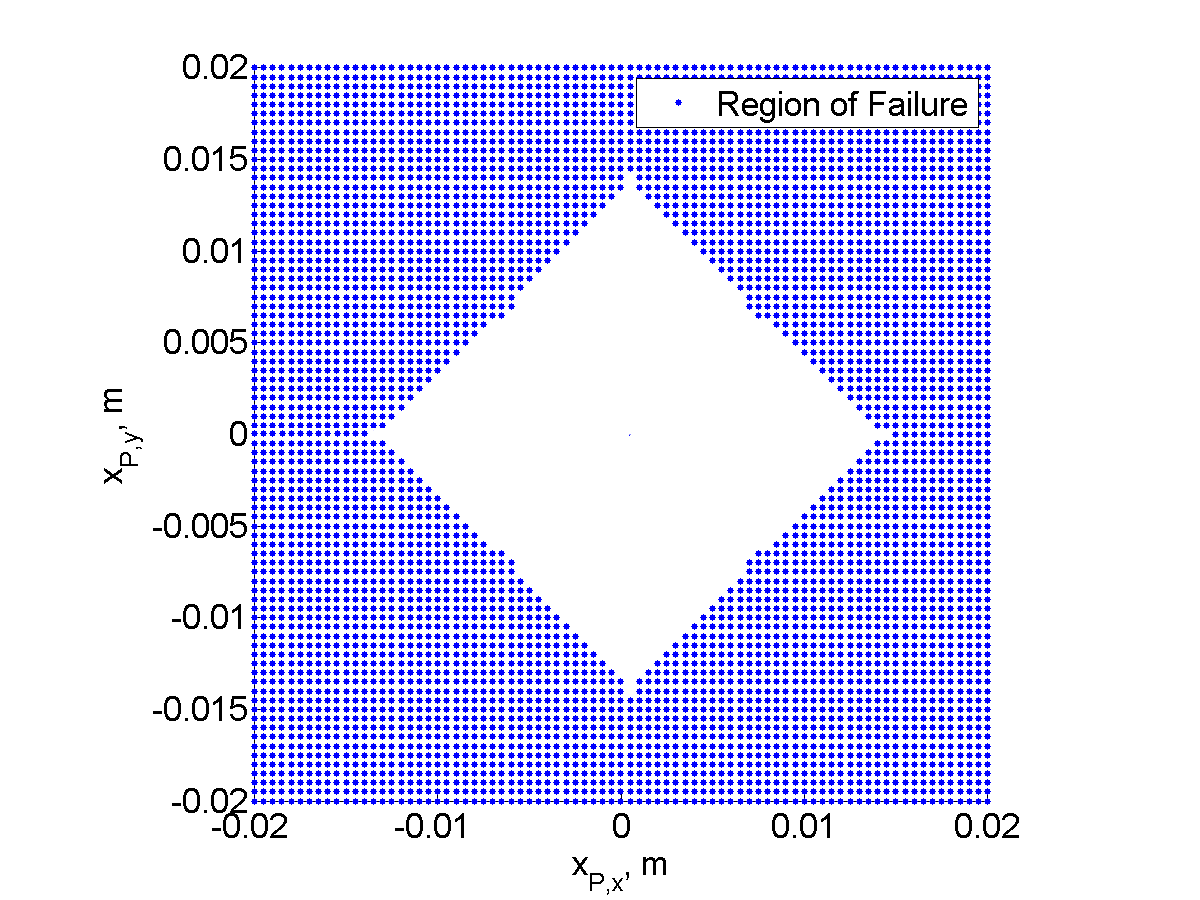
\includegraphics[width=0.495\textwidth]{pos_rom.png}}
				\fbox{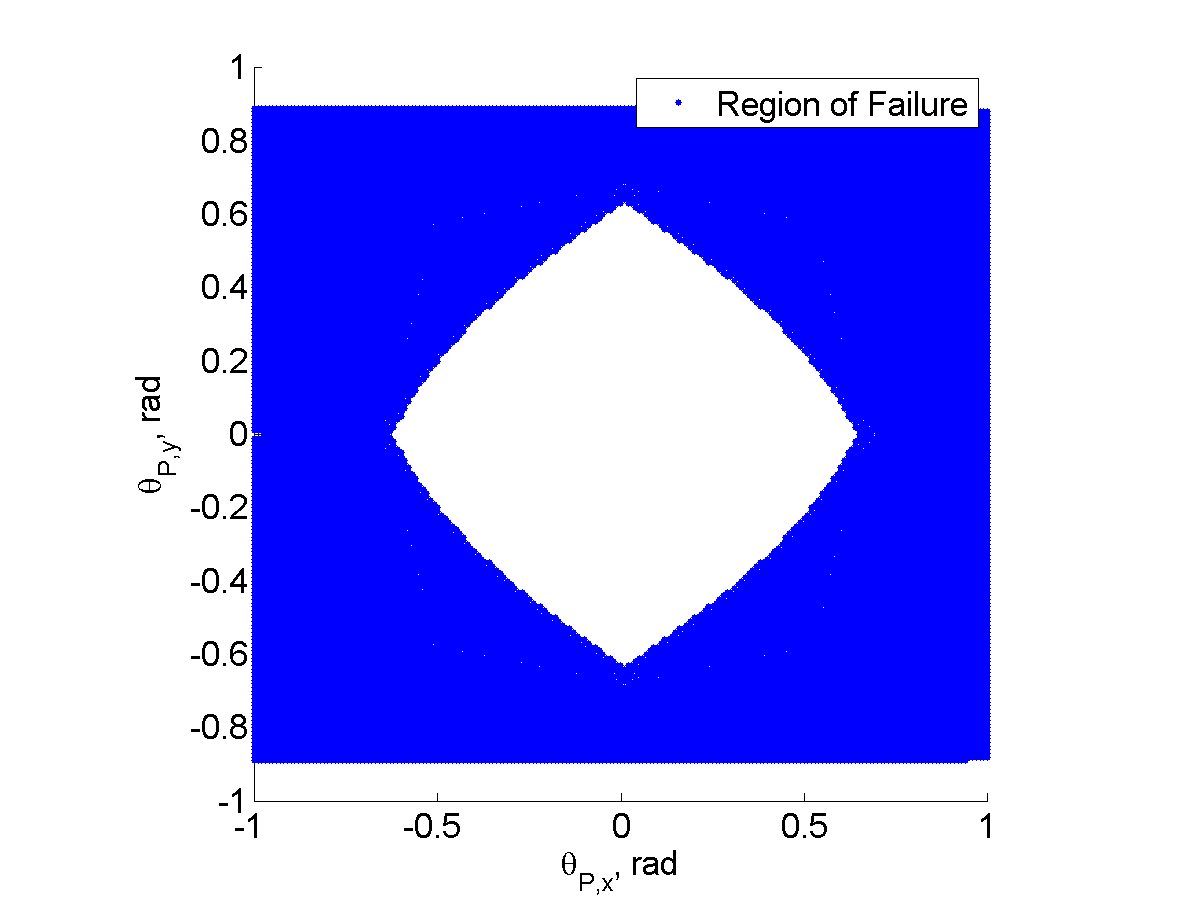
\includegraphics[width=0.495\textwidth]{ori_rom.png}}
				\caption{Range of motion for body's planar position (\emph{left}) and body pitch and roll (\emph{right}) while in the default stance.}
				\label{fig::pos_and_ori_rom}
			\end{figure}
			It can be seen from Figures \ref{fig::pos_and_ori_rom} that the platform can achieve a maximum pitch and roll of  $\pm37^o$and a total displacement of $\pm 1.4 \text{ cm}$ along the \emph{x} and \emph{y} axis of $O_{b'}$.


		\subsection{Velocity Kinematics}

			Using the DH-coordinate transformation, ${H}^{i,0}_{i,4}$, the velocity kinematics of each \Ith leg are derived as the Jacobian $J^{i,0}_{i,e} \InRe{6\times4}$ where 
				\begin{equation}
					\dot{x}^{i,0}_{i,e} = J^{i,0}_{i,e}  \dot{q}_{i}
					\label{eq::leg_jacobian}
				\end{equation}
			with $\dot{x}^{i,0}_{i,e} \InRe{6}$ being stacked vector of translational and rotational velocities, $\dot{p}_{i,e}^{i,0} \InRe{3}$ and $\dot{\theta}_{i,e}^{i,0}\InRe{3}$, respectively, of each \Ith foot with respect to frame $O_{i,0}$. The matrix $J^{i,0}_{i,e}$ is defined explicitly in Appendix \ref{appendix::a}.

			Assuming the translational and rotational velocity of the trunk, $\dot{p}_{b}$ and $\dot{\theta}_{b}$, respectively; and the translational and rotational of each \Ith foot, $\dot{p}_{i,e} \InRe{3}$ and $\dot{\theta}_{i,e} \InRe{3}$, respectively, are known, the translation velocity of each \Ith foot can be written with respect to frame $O_{i,0}$ by:
				\begin{equation}
					\dot{p}_{i,e}^{i,0} \equiv \wrap{R^{0}_{i,0}}^{T} \wrap{ \dot{p}_{i,e} - \dot{p}_{b} - \Skew{ \dot{\theta}_{b} } \wrap{ {p}_{i,e} - {p}_{b} - R^{0}_{i,0} \vec{o}_{\nu} } }
				\end{equation}
			where $\vec{o}_{\nu} = [\nu,0,0]^{T}$, $R^{0}_{i,0}$ is the rotation-matrix component of the transformation $H^{0}_{i,0}$ defined in \ref{eq::world_to_dh}, and $\Skew{*}$ is a skew-symmetric matrix operator, which takes a $3\times1$ vector input. The corresponding rotational velocity of each \Ith foot  can be computed with respect to $O_{i,0}$ by:
				\begin{equation}
					\Theta^{i,0} \equiv \wrap{ R^{0}_{i,0} }^{T} \Skew{ \dot{\theta}_{i,e} - \dot{\theta}_{b} } R^{0}_{i,0}  = \Skew{ \dot{\theta}^{i,0}_{i,e} }
				\label{eq::velocity_skew}
				\end{equation}
			where the rotational velocity of each foot, described by $\dot{\theta}^{i,0}_{i,e}$, is recovered by:
				\begin{equation}
					\dot{\theta}^{i,0}_{i,e} \equiv \sbrack{ 
						-\Theta^{i,0}_{1,2},
						 \Theta^{i,0}_{1,3},
						-\Theta^{i,0}_{2,3}
					}^{T}
				\end{equation}
			with $\Theta^{i,0}_{j,k}$ being the \Kth element in the \Jth row of the skew symmetric matrix $\Theta^{i,0}_{j,k}$ which results from \ref{eq::velocity_skew}.

			Joint velocities required to attain $\dot{x}^{i,0}_{i,e}$ can be computed using $J^{i,0}_{i,e}$. However, since each of BlueFoot's of legs has 4 degrees of freedom, $J^{i,0}_{i,e}$ is rank deficient and $\dot{q}_{i}$ cannot be obtained by direct inversion. Instead, $\dot{q}_{i}$ can be approximated from $\dot{x}^{i,0}_{i,e}$ by a weighted, Penrose-Moore psuedo-inverse of $J^{i,0}_{i,e}$, which is defined as follows:
				\begin{eqnarray}
					\dot{q}_{i} &\approx& \sbrack{J^{i,0}_{i,e}}_{\Lambda_{j}}^{\dagger} \dot{x}^{i,0}_{i,e} \nonumber \\
					\dot{q}_{i} &\approx& \wrap{ \wrap{J^{i,0}_{i,e}}^{T}J^{i,0}_{i,e} + \Lambda_{J} }^{-1} \wrap{J^{i,0}_{i,e}}^{T}\dot{x}^{i,0}_{i,e}
				\end{eqnarray}
			where $\Lambda_{J}$ is a strictly positive-definite weighting matrix that is typically chosen to have 
				\begin{equation*}
					\text{det}(\Lambda_{J}) \ll 1.
				\end{equation*}
			The operator $\sbrack{*}_{\Lambda_{j}}^{\dagger}$ defines a weighted pseudo-inversion off a matrix argument $(*)$ given a positive-definite weighting matrix $\Lambda_{j}$. A weighted pseudo-inversion is chosen over direct pseuedo-inversion to avoid a non-smooth set of solutions $\dot{q}_{i}$. Degenerate solutions for $\dot{q}_{i}$ exist at particular manipulator configurations where $\wrap{\wrap{J^{i,0}_{i,e}}^{T}J^{i,0}_{i,e}}$ is non-invertible.




	\section{Dynamical Model}
	

		\subsection{System State Vector and General-Form Dynamics}
		
			The dynamical model of the BlueFoot platform is treated a general, free-floating body with four ridged legs, each of which have four degrees of freedom. This system is fully described by the state vector $z \equiv [\eta^{T}, \dot{\eta}^{T}]^{T} \RealVec{44}$ and its dynamics are:
				\begin{equation}
					M(\eta)\ddot{\eta} + C(\eta,\dot{\eta})\dot{\eta} + G(\eta) + \Delta{H} = \tau + J^T(\eta) f_{ext} %
					\label{eq::normal_form_dynamics}
				\end{equation}
			where $M(\eta)$, $C(\eta,\dot{\eta}$), $G(\eta)$ and $J(\eta)$ represent the system mass matrix, Coriolis matrix, gravity matrix and Jacobian, respectively \cite{Wieber2006}. $\Delta{H}$ has been included as a lump term to account for dynamical uncertainties, such as friction or unmodeled coupling effects. Additionally, $f_{ext} = [ f_{1,ext}^{T},f_{2,ext}^{T},f_{3,ext}^{T},f_{4,ext}^{T}]^{T} \RealVec{24}$ represents a stacked vector of force-wrenches, $f_{i,ext} \RealVec{6}$, applied to the system through each \Ith foot. The state vector, $\eta$, can be partitioned as follows: $\eta = [ {p}_{b}^{T}, \theta_{b}^{T}, q^{T} ]^{T}$ with ${p}_{b} \RealVec{3}$ and $\theta_{b} \RealVec{3}$ representing the position and orientation, respectively, of the quadruped's trunk in an arbitrarily placed world coordinate frame, and $q \RealVec{16}$ is a vector of joint variables, $m$ of which are contributed by each leg. $\tau \RealVec{22}$ represents a vector of generalized torque inputs and takes the form $\tau = [ 0_{1x6}, \tau_{q}^{T} ]^{T}$ where $\tau_{q}$ represents a set of torque inputs to each joint. It is important to note that the states we are most interested in controlling, ${p}_{b}$ and $\theta_{b}$, are not directly actuated, and must be controlled via composite leg joint motions.		

			BlueFoot's dynamics, from \ref{eq::normal_form_dynamics}, can be realized in a general, compact, state-space form by:
				\begin{equation}
					\begin{split}
					\dot{z}_{1} 				&= z_{2} \\
					\dot{z}_{2} 				&= M^{-1}(z_{1})(\tau + \Phi(z_{1},z_{2},f_{ext})) \\
					\Phi(z_{1},z_{2},f_{ext}) 	&= J^T(z_{1}) f_{ext} - C(z_{1},z_{2})z_{2} - G(z_{1}) - \Delta{H}
					\end{split}
					\label{eq::state_space_dynamics}
				\end{equation}
			where $z_{1}=\eta$ and $z_{2}=\dot{\eta}$. The notation $\Phi(z_{1},z_{2},f_{ext})$ is introduced for convenience as a composite dynamical term. This term will be referred to, simply, as $\Phi$ in the sections that follow. The system dynamics are also considered in an approximate, discrete-time (first-order) form as follows:
				\begin{equation}
					\begin{split}
					{z}_{1,k+1} &= {z}_{1,k} + ( {e}_{1,k}^{\Delta_{s}} + {z}_{2,k} )\Delta_{s} \\
					{z}_{2,k+1} &= {z}_{2,k} + M^{-1}_{1,k}( {e}_{2,k}^{\Delta_{s}} + \tau_{k} + \Phi_{k}) \Delta_{s} \\
					t 			&= \Delta_{s} k
					\end{split}
					\label{eq::sampled_dynamics}
				\end{equation}
			where $M_{1,k} = M(z_{1,k})$ and $\Delta_{s} \equiv (f_{s})^{-1}$ with $f_{s}$ defining a uniform sampling frequency in Hz. The terms ${e}_{1,k}^{\Delta_{s}}$ and ${e}_{2,k}^{\Delta_{s}}$ are used to explicitly account for system discretization errors, which vary with respect to the step-size, $\Delta_{s}$. 

		\subsection{Joint-Servo Dynamics}

			The motor dynamics driving each joint need to be considered for use in control design since the input to BlueFoot's servo motors at each joint is a reference position command. In model-based control schemes to follow, a simple model of the motor dynamics will be utilized. Moreover, servos are considered as simple torque generators of the following form:
				\begin{equation}
					\tau_{q} = k_{s}(q^{r}-q)
					\label{eq::servo_control_dynamics}
				\end{equation}
			where $k_{s}>0$ is a constant, scalar gain and $q^{r}$ is a joint position reference. The servos being utilized to drive the leg joints of the BlueFoot quadruped have high-gain position feedback which allows us to model the motors, simply, as a static block which transform reference trajectories to torque outputs. All of these servos are identical, and thus have identical gains. One could instead consider the full motor dynamics for computing reference positions given a desired torque. The simple model stated above was adequate for achieving desired results with all proposed control schemes which use this torque-generator model.


		\subsection{Single Leg Dynamics}
			
			The dynamics of each independent leg (with each base-frame fixed) can be derived in closed form using a Lagrangian formulated using the total potential and kinetic energy. Here, the dynamics of each leg is formulated via a minimization of energy. Masses $m_{i,j}$ along each \Ith leg are taken to be centered at each \Jth joint. These dynamics have been included as auxiliary matter in Appendix~\ref{appendix::b} using the previously defined notations.


	\section{BlueFoot Simulator}

		\begin{figure}[h!]
			\centering
			\fbox{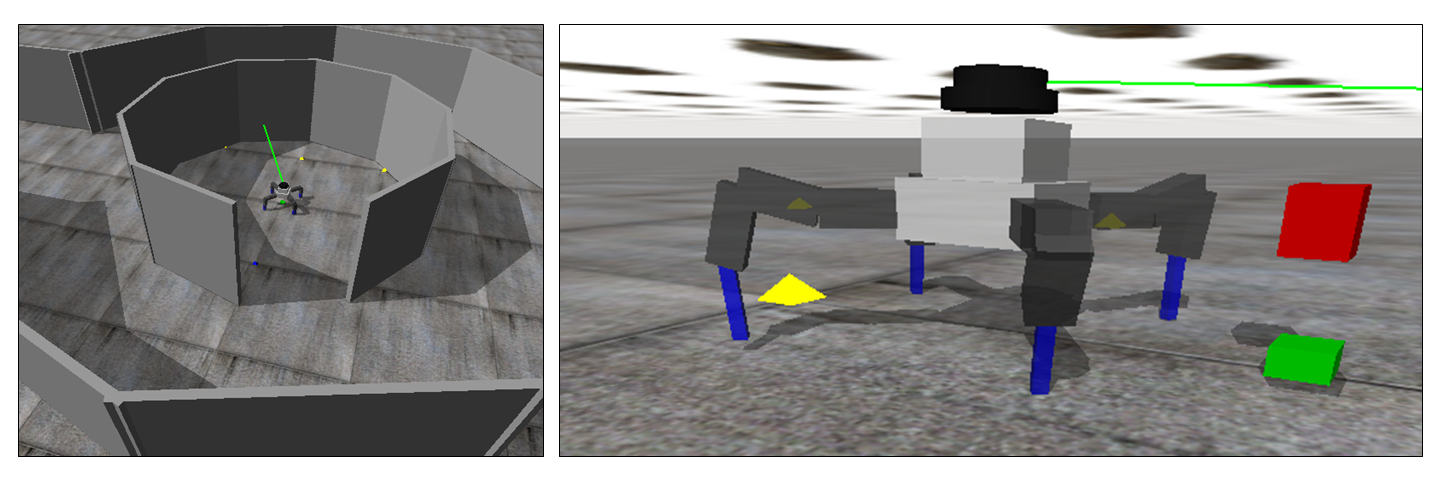
\includegraphics[width=1.00\textwidth]{simulation_wide_pic.png}}
			\caption{Visualization of the BlueFoot simulator.}
			\label{fig::simulator_wide}
		\end{figure}

		The BlueFoot platform is comprised of 17 rigid bodies, 16 of which are linkages between joints; and a main platform. Since each limb is formed from four revolute joints, the system has a total of 22 DOF, 16 of which are actuated. The main platform's configuration is generated through particular configurations of the legs. Furthermore, because each linkage is constrained to a rotation about a single axis, the rigid-body dynamic model of the BlueFoot quadruped is represented by 44 states. These states represent the position and velocity of each joint, $q_{i}$ and $\dot{q}_{i}$, respectively. Additionally, foot contact states are represented by binary scalars, $\mu_{i} \in \wrap{0,1}$, which describes whether the foot is not in contact or in contact, respectively.

		The dynamics of this system are somewhat complex because the quadruped's legs continuously make and break contact with the ground during gaiting. Additionally, the surface attributes and contact effects may vary significantly during gaiting and for various environments. A numerical dynamics engine, Open Dynamics Engine (ODE) \cite{ODE_Website}, has been utilized to implement a dynamics simulator for the BlueFoot platform. The simulator allows for various reconfigurations of environmental parameters, such as joint-friction, body-contact friction, and physical obstacles. Additionally, this simulation environment is implemented with a variety of geometric collision solvers and and efficient collision search method.

		The simulator's numerical engine, based on ODE is updated at 1000 Hz to attain high-fidelity, especially during contact phases, which require higher-than-normal integration stability to achieve reasonable  simulation accuracy. The input to the simulator is the desired main body configuration (i.e., position and orientation); desired foot placements; and desired ankle orientations, from which an inverse kinematic model is solved to attain all the desired joint configurations for the legs. Servos at each joint have built-in, tunable proportional controllers that effectively render them as ideal torque generators responding to the command input, as depicted in \ref{eq::servo_control_dynamics}. To mimic the behavior of the system, the commands to each joint motor are updated at 50 Hz, which matches the update rates at which the actual robot serves the P-controllers at each joint with reference positions. This rate has been chosen to account for the speed of inter-processor communications, and is adequate given the operating bandwidth of the robot.
		
		The BlueFoot simulator utilizes a dynamical model of the platform which consists of purely rectangular bodies. To match the dynamics of the true system, the individual mass and inertia parameters of each rigid body have been generated using a 3D model analysis software. This software takes into account geometric irregularities and variation of materials when computing the inertia of each body. The simulator also contains IMU and LIDAR sensor models for gathering feedback from the simulated environment. Each sensor is modeled with appropriate measurement noise so as to more closely match the performances of the actual IMU and LIDAR sensors on-board the BlueFoot platform.

			\begin{figure}[!h]
				\centering
				\fbox{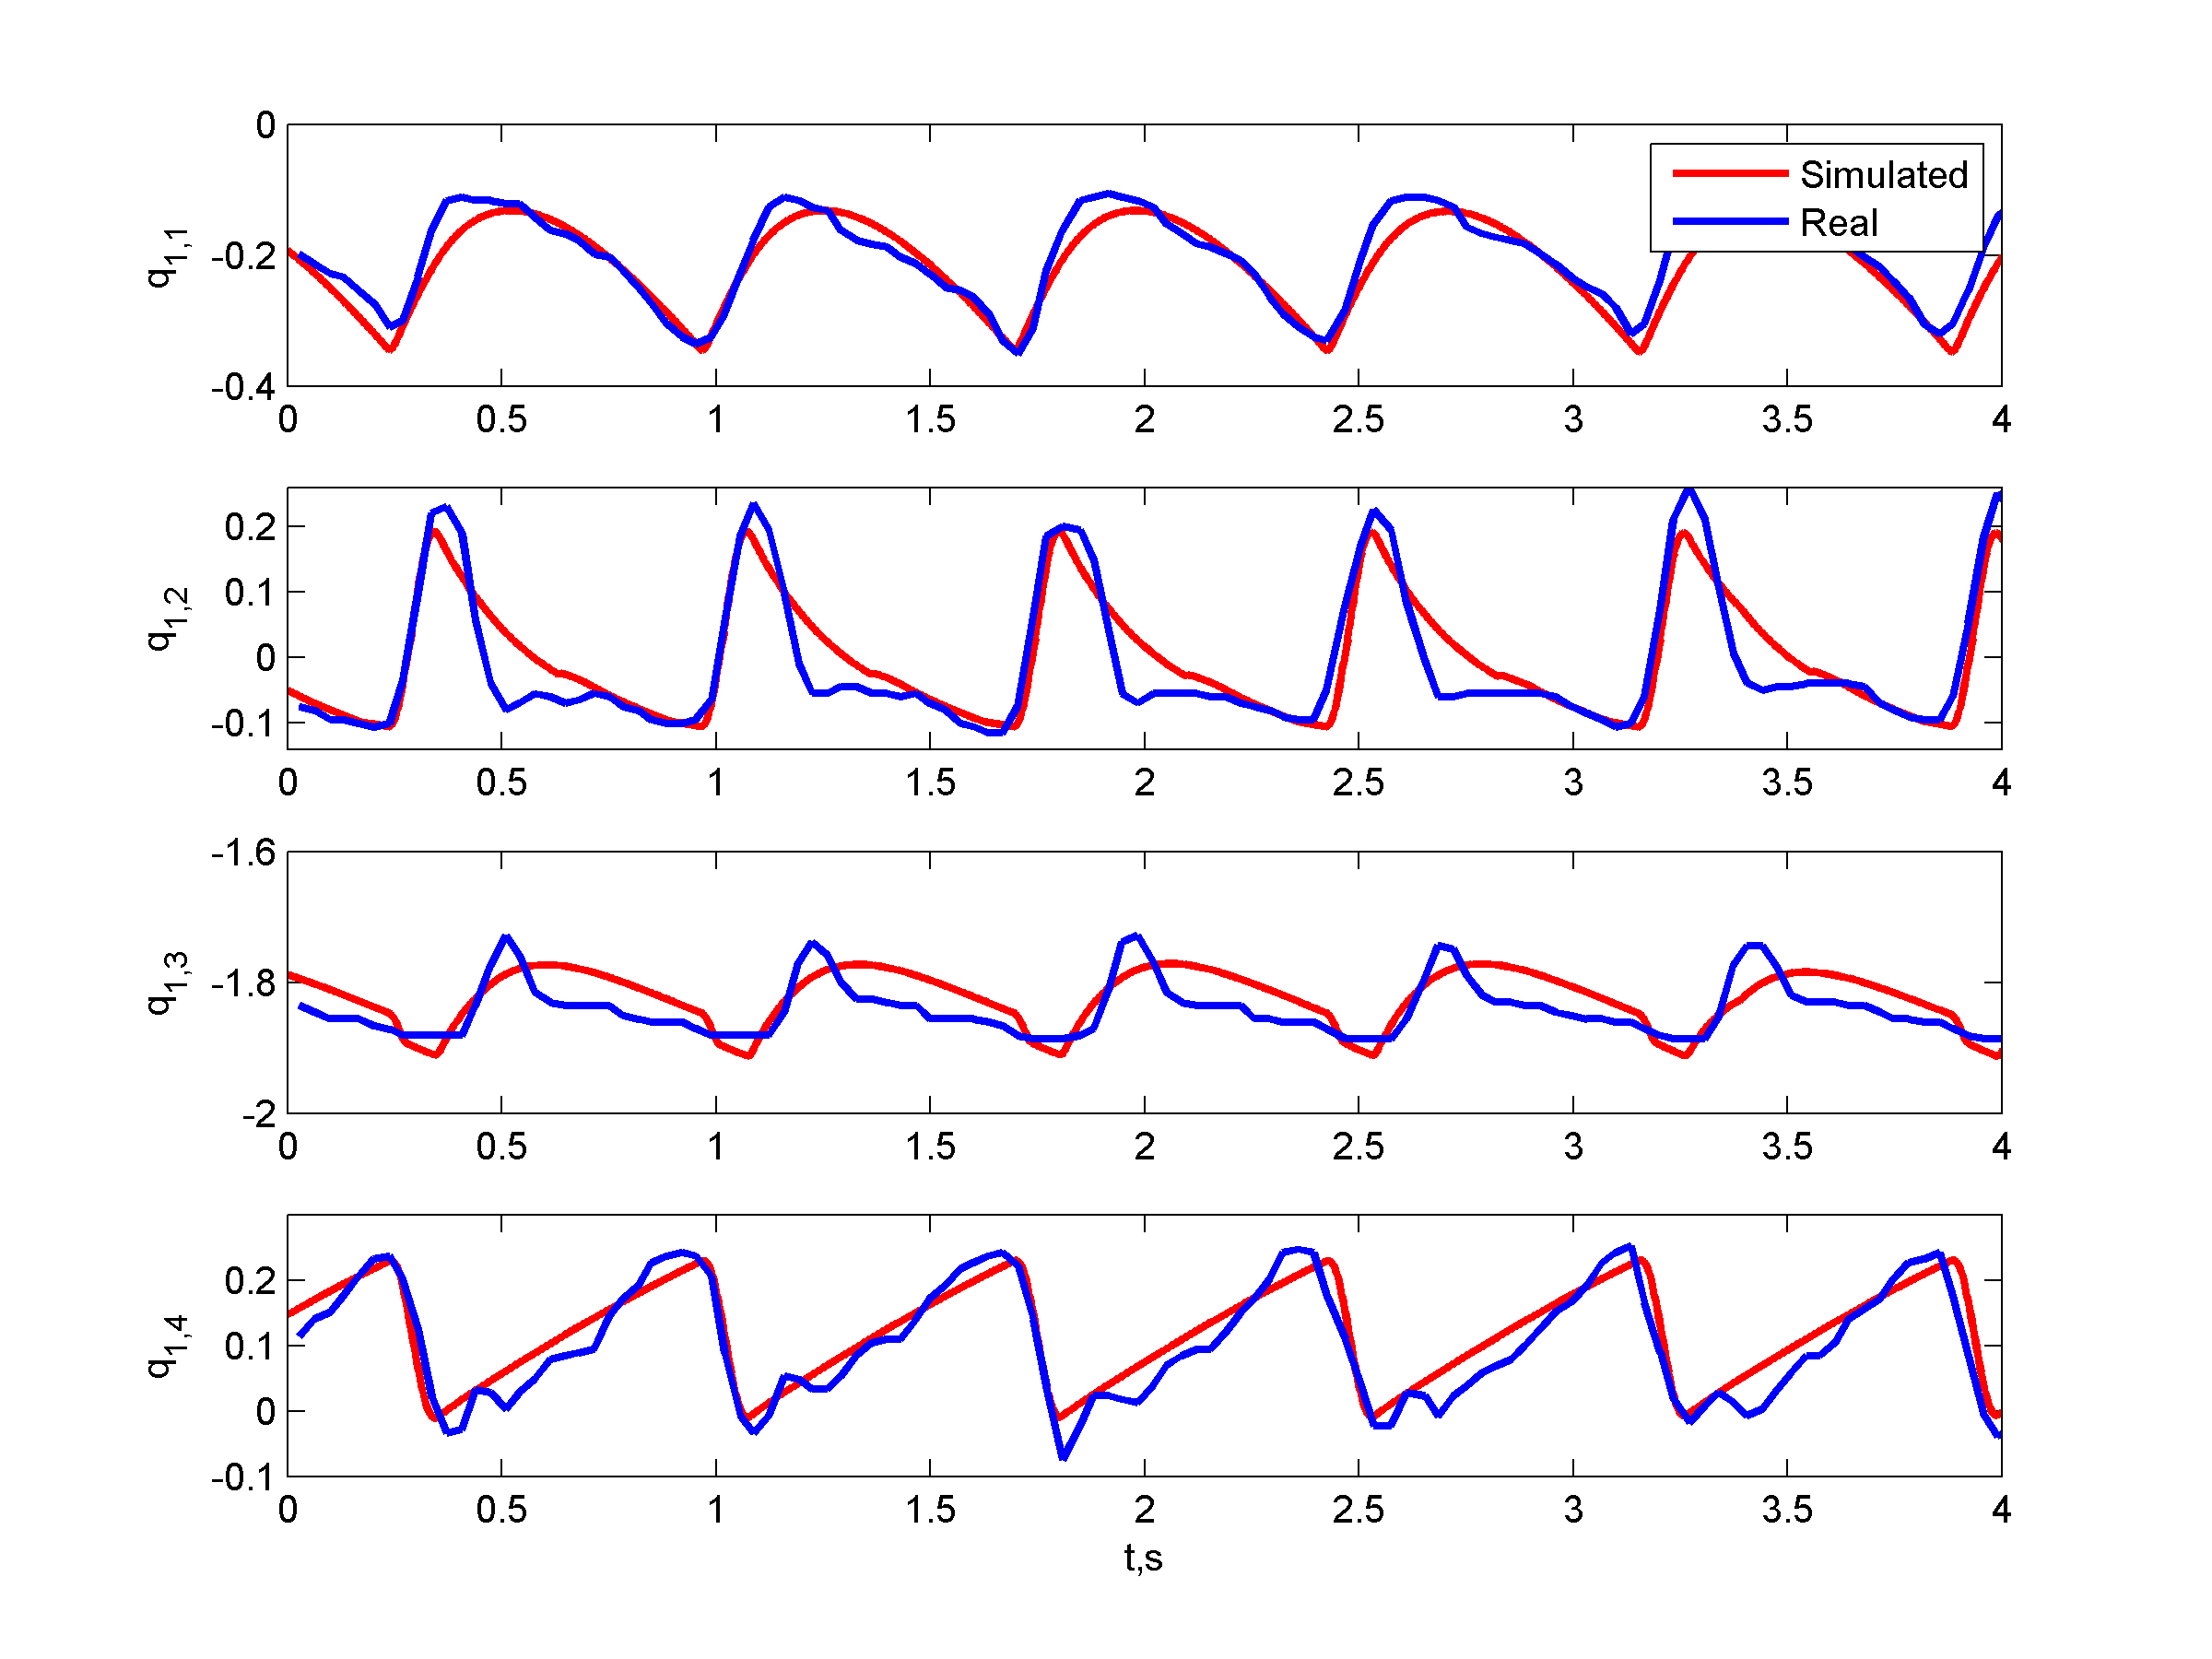
\includegraphics[width=1.00\textwidth]{sim_comparison.png}}
				\caption{Joint position comparison between the simulated and real quadruped while performing a gait which achieves a forward velocity of $60\frac{mm}{s}$}
				\label{fig::sim_performance_comparison}
			\end{figure}

		Careful, manual tuning was performed on simulated robot parameters, including joint update gains, joint-friction and surface-friction model coefficients to achieve closer matches between simulated results and the actual robot motions. A performance comparison can be seen in \ref{fig::sim_performance_comparison}, which shows joint position outputs for all joints of the front-right leg of the actual and simulated robot while performing a forward gait at $0.060$ m/s. It can be seen in  that the simulator provides and approximate representation true system performance within some margin of error. The discrepancies between the two data sets can be seen to usually occur at the minima of each series when the robot makes contact with the ground after a step. These differences can be attributed to ground-contact model inaccuracies. Work is still left to be done in improving the simulator's contact model, but this is more the fault of the simulation software libraries being used, namely in its low-order contact models. These contact models are very simplistic for the sake of simulation speed. Contact models could certainly be improved such that they more closely matches the effects of real-world surfaces. Additionally, discrepancies could also be attributed to the low-order joint model being used to represent the system's servo motors at each joint, described in \ref{eq::servo_control_dynamics}. This model neglects the effects of higher-order frictional effects which modify the rotation profile at each joint. All of the other simulated leg joints exhibited similar results to the actual motions.

		Despite these discrepancies, this simulation platform has proven to be adequate for use in testing gaiting and control algorithms which have been implemented on the real system. Moreover, all motion control algorithms which were first developed in this simulated environment have been ported to the real robot platform and performed in a highly comparable manner.

		The simulator has also been utilized to model BlueFoot's on-board LIDAR unit for use in testing navigation and terrain mapping algorithms and associated motion routines. Laser hits are modeled as force-less collisions between a ray-type geometry, used to represent the laser beam of the LIDAR, and environmental elements. Because the ray geometry can penetrate environmental elements in multiple places, or even multiple elements within the environment at a single instance, some post processing is performed on collision point returned by the simulator such that the point of intersection \emph{closest} to the robot is taken as a laser-beam hit. Additionally, sensor realism is imposed by limiting the data access frequency to buffered laser data by control routines operating the simulated robot to a rate of 10 Hz, which matches the scan rate of BlueFoot's on-board LIDAR. The angular velocity of the spinning laser head and the depth of each laser beam hit are corrupted by zero-mean Gaussian random noise with variances close to the parameters specified in the datasheet of the LIDAR unit.

	\chapter{Gaiting and Gait-Stability Control}
	\label{ch::gait_control}
	

	\section{Overview}

		Legged robotic systems have long employed motion controllers based on limit cycle oscillators and, more recently, Central Pattern Generators (CPGs)  for the purpose of generating bio-mimetic gaits \cite{Matsuoka1985,Collins1993,Endo2004,Righetti2006,Ijspeert2008,Matos2010,Ajallooeian2013,Park2014,Fukuoka2015}. Since these motion control methods are open-loop motion planners (\IE not inherently formulated to incorporate feedback) they do not perform any active system stabilization on their own accord. As a result, implementations involving these  locomotion methods often require auxiliary control mechanisms which provide gait stability. Fixed point methods, which include considerations of the system's zero-moment point (ZMP) and center of gravity (COG), are utilized in the design of stable oscillator driven gaits. These methods are summarized in \cite{Wieber2015}. %add ZMP references%

		Developments in CPG-based gait controllers have led to the incorporation of ``reflexive" feedback mechanisms aimed at correcting foot-placement during gaiting on uneven terrain or various surfaces. One such approach involves active compliance to each leg by directly modifying CPG oscillators units through feedback-driven modulations. In \cite{Fukuoka2003,Endo2004}, a CPG for each leg is modified by a neural oscillator with one tuning parameter. 

		This chapter will detail a similar, reflex-adaptive CPG gait generation method which utilizes IMU feedback to modify CPG limit-cycle parameters. Additionally, this section will present related motion-control methods implemented on the BlueFoot platform which aid in gait stabilization, including a virtual force-based foot placement planner and a ZMP-based body placement controller; as well as a learning-based control technique used to level BlueFoot's trunk during gaiting.


	\section{Central Pattern Generator (CPG) Based Gaiting}

		A central pattern generator (CPG), which includes a reflexive mechanism using sensory feedback, is utilized as the core of the robot's gait generation algorithm. CPGs are a form of neural oscillator network which mimic biological mechanisms for repetitive motor tasks \cite{Ijspeert2008,Collins1993}. CPGs commonly consist of a network of multi-state unit-oscillators. These unit-oscillators are coupled such that the motion of one oscillator drives or attenuates the motion of other oscillators it is connected to, creating phase-locked limit cycles.

		In this context, the limit-cycles generated with a CPG will be utilized to drive a quadruped  walking gait by mapping oscillator outputs to foot position controls. CPGs are widely used in this way as they provide a compact method for prescribing rhythmic gaits with variable stepping sequences 
		\cite{
			Righetti2006,
	 		Castro2008,
			Li2014
		}. 
		CPG-driven gait controllers are convenient as they allow for continuous transitioning between gaiting patterns through the modification of oscillator coupling. Reflexes are built into the oscillators which use IMU measurements to modulate the CPGs unit oscillators, as will be outlined later in this section.

		The CPG implemented on BlueFoot consists of four modified two-state Hopf Oscillators connected through a coupling matrix $K$. The states of each \Ith unit Hopf Oscillator are designated by the pair $\{y_{1,i},y_{2,i}\}$. These oscillator states are stacked into the vectors $y_{1}\in \Re^{4}$ and $y_{2}\in \Re^{4}$, which are composed as follows:
	\begin{eqnarray*}
		y_{1} &=& \sbrack{y_{1,1},y_{1,2},y_{1,3},y_{1,4}}^{T}\nonumber\\
		y_{2} &=& \sbrack{y_{2,1},y_{2,2},y_{2,3},y_{2,4}}^{T}
	\end{eqnarray*}
The oscillator output vector $y_{2}$, parameterizes the trajectories of each \Ith foot. The resulting reflexive CPG system, written which respect to the stacked-state vectors $y_{1}$ and $y_{2}$, is described by
		\begin{eqnarray}
			\dot{y}_{1} &=& A_{1}\wrap{ \Psi_{M} M\wrap{y_{1},y_{2}} - \Gamma}{y}_{1} + \Psi_{\omega} W {y}_{2} 			\nonumber\\
			\dot{y}_{2} &=& A_{2}\wrap{ \Psi_{M} M\wrap{y_{1},y_{2}} - \Gamma}{y}_{2} - \Psi_{\omega} W {y}_{1} + K {y}_{2}	%\nonumber
			\label{eq::cpg_ss_def}
		\end{eqnarray}
		where $M\wrap{y_{1},y_{2}} \in \Re^{4\times4}$ is defined as
		\newcommand{\yy}[1]{y_{1,#1}^{2} + y_{2,#1}^{2}}
		\begin{equation*}
			M\wrap{y_{1},y_{2}} = \left[
			\begin{array}{cccc}
			\yy{1} 	& 	0 		& 	0 		& 	0 		\\ 
			0		& 	\yy{2}  & 	0 		& 	0 		\\ 
			0 		& 	0 		& 	\yy{3}  & 	0 		\\ 
			0 		& 	0 		& 	0 		& 	\yy{4}  \\ 
			\end{array}
			\right],
		\end{equation*}
${A_{1},A_{2}, \Psi_{M}, \Psi_{\omega}} \InRe{4\times4}$ are constant oscilattor gain matrices; and $\Gamma$ and $W$ are diagonal matrices, defined by
		\begin{equation*}
			\Gamma = \left[
			\begin{array}{cccc}
			\gamma_{1} 	& 	0 				& 	0 				& 	0 		\\ 
			0				& 	\gamma_{2} 	& 	0 				& 	0 		\\ 
			0 				& 	0 				& 	\gamma_{3} 	& 	0 		\\ 
			0 				& 	0 				& 	0 				& 	\gamma_{4}  \\ 
			\end{array}
			\right],
			\Sep
			W = \left[
			\begin{array}{cccc}
			\omega_{1} 	& 	0 				& 	0 				& 	0 		\\ 
			0				& 	\omega_{2} 	& 	0 				& 	0 		\\ 
			0 				& 	0 				& 	\omega_{3} 	& 	0 		\\ 
			0 				& 	0 				& 	0 				& 	\omega_{4}  \\ 
			\end{array}
			\right],
		\end{equation*}
which define the peak-to-peak output amplitude, $\gamma_{i}$, and frequency, $\omega_{i}$, of each \Ith unit oscillator in the CPG network. A more specific design of the matrix $W$, with respect to a gait frequency parameter, $\omega_{s}$, is provided in \ref{eq::cpg_W_matrix_def}.


		\subsection{Reflexive Gait Adaptations}

			Feedback signals are incorporated into the CPG through the frequency modulation matrix $\Psi_{\omega}$ and amplitude modulation matrix $\Psi_{M}$. These modulation parameters are generated using state estimates of the platform's orientation and angular rate. The platform orientation state-estimate, $\hat{\theta}_{b}$, is supplied to the controller from an Extended Kalman Filter utilizing inertial measurement and magnetometer feedback (which are separately calibrated). The platform's angular rate is output by an angular rate-gyro sensor.

			Feedback-based corrections to the CPG aid in tracking a specified body orientation $\theta_{b}^{r}$ during gaiting. To achieve higher system velocities, it is often necessary to perform a gait wherein multiple legs leave contact with the ground. Configurations such as these would cause a quadruped robot to tip in the direction of the non-planted legs, thus disturbing $\theta_{b}$. These disturbances are counteracted, in part, by adjusting the CPG such that the amount of torque applied on the main body by legs in flight is actively limited. This is done by adjusting stepping height and time-of-flight according to a measure of disturbance (essentially, the amount and rate of tipping). These adjustments have been formulated to mimic reflexive behaviors that might be performed by a biological system.

			When the robot's body begins to fall in particular direction (\IE is disturbed by legs in-flight during gaiting), the disturbance signal 
		\begin{equation}
			\dot{\epsilon}_{\theta} = {R}_{z_{b}}\wrap{\frac{\pi}{2}}\wrap{\dot{\hat{\theta}}_{b} - \dot{\theta}_{b}^{r}}
		\end{equation}
			is non-zero. $\dot{\epsilon}_{\theta}$ represents a measure of translational drift recovered from gyroscopic sensor measurements. ${R}_{z_{b}}{\frac{\pi}{2}}$ represents a rotation by $\frac{\pi}{2}$ about the z-axis of the body frame $O_{b}$. $\dot{\epsilon}_{\theta}$ is mapped to the parameters $\Psi_{\omega}$ and $\Psi_{M}$ by
				\begin{eqnarray}
					\psi_{i} 			&=& \Sig{  w_{i} \emph{T}_{i} - w_{i} c_{i} } {\mu}_{i} 	\nonumber\\
					\Psi_{\omega} 		&=& I + A_{\omega}\DiagMat{ \psi_{i} } 						\nonumber\\
					\Psi_{M}			&=& I - A_{\mu} \DiagMat{  \psi_{i} } 
					\label{eq::cpg_modulations}
				\end{eqnarray}
			where
				\begin{eqnarray}
					\emph{T}_{i} 		&=& \norm{ \dot{\epsilon}_{\theta} } \wrap{1 + \Normalize{\Delta x_{i}}^T  \Normalize{ \dot{\epsilon}_{\theta}  } }	\nonumber\\\
					\Delta x_{i}		&=& {p}_{e} - {p}_{b}
				\end{eqnarray}
			with $\{w_{i}, c_{i}\} \InRe{}$ and $\{A_{\mu}, A_{\omega}\}   \InRe{4\times4}.$ $\Sig{*}$ represents the standard
			sigmoid step function. The signal $\emph{T}_{i}$ represents a projection of $\dot{\epsilon}_{\theta}$ into the unit-vector emanating from ${p}_{b}$ to each \Ith foot. This projection delegates the level of adjustment to each \Ith oscillator as a result of $\dot{\epsilon}_{\theta}$. 		

			Adjusting $\Psi_{\omega}$ by the method delineated in \ref{eq::cpg_modulations} serves to shorten the stepping period of a leg in-flight given greater values of $\dot{\epsilon}_{\theta}$. Likewise, $\Psi_{M}$ is adjusted to decrease the height of each foot in-flight. 

			The frequency of a full gaiting cycle is prescribed via $\omega_{s}$ and duty-factor $\alpha \in \sbrack{0,1}$ \cite{Matos2010}. The matrix $W$ is formed from  $\omega_{s}$ and $\alpha$ as a follows:
				\newcommand{\Wel}[1]{\frac{1}{1+e^{#1}}}
				\begin{equation}
						W = 
						\omega_{s}\alpha 
						\left[	
							\begin{array}{ccc}
								\Wel{\zeta y_{2,1}} 		& 0 			& 0  \\
								0 							& \ddots 		& 0  \\
								0							& 0		 		& \Wel{\zeta y_{2,4}}
							\end{array}
						\right] + 
						\omega_{s}(1-\alpha) 
						\left[	
							\begin{array}{cccc}
								\Wel{-\zeta y_{2,1}} 		& 0 			& 0  \\
								0 							& \ddots 		& 0  \\
								0							& 0		 		& \Wel{-\zeta y_{2,4}}
							\end{array}
						\right]
					\label{eq::cpg_W_matrix_def}
				\end{equation}
			and $\zeta$ being a sensitivity tuning parameter. A linear mapping between commanded platform velocity, $v^{r}$, and $\omega_{s}$ is prescribed such that stepping-cycle frequency is adjusted proportionally with respect to the desired velocity of the system, \IE $\omega_{s} = a_{v}v^{r}$.

			In BlueFoot's CPG implementation, the coupling matrix $K$ takes on the values $k_{i,j} \in \sbrack{-1,1}$. Each element of the coupling matrix, $k_{i,j}$, is utilized to adjust the phase offsets between the unit-oscillators.Furthermore, setting $k_{i,j}=1$ causes the \Jth oscillator to attract the \Ith oscillator  towards a  positive peak, and vice-versa. Setting $k_{i,j}=0$ effectively disconnects \Ith and \Jth oscillators. 

			Figures~\ref{fig::cpg_phase2_45} and \ref{fig::cpg_phase4_45} depict the CPG output, $y_{2}$, and corresponding unit-oscillator phase portraits of the oscillator dynamics, given by \ref{eq::cpg_ss_def} with the feedback mechanism given in \ref{eq::cpg_modulations} used during simulations of BlueFoot's default two-pace trotting and four-pace walking gaits, respectively. The associated $K$ matrix prescribing this gaiting pattern is a modified version of $K$ for a 2-pace trot gait presented in \cite{Rutishauser2008}, since this generates a more effective and fluid gait when applied to BlueFoot's gait controller
				\begin{equation}
						K\equiv 
						\left[ 
						\begin{array}{cccc}
						 0	   	&	-1   	&	 	 1   	&		-0.5\\
						-1	   	&	 0   	&	 	-0.5   	&		 1 	\\
						-1    	&	-0.5   	&		0    	&	 	-1 	\\
						-0.5	&	 1   	&		-1    	&		 0
						\end{array}
						\right].
						\label{eq::K_two_pace}
				\end{equation}
			A comparable four-pace \emph{walking} gait can be achieved by a slight sign modifications on the elements of  \ref{eq::K_two_pace}, which yields \ref{eq::K_four_pace} as follows:
				\begin{equation}
						K\equiv 
						\left[ 
						\begin{array}{cccc}
						 0	   	&	-1   	&	 	 1   	&	  	-0.5\\
						-1	   	&	 0   	&	 	-0.5   	&		 1 	\\
						-1    	&	 0.5   	&		 0    	&	 	-1 	\\
						 0.5	&	-1   	&		-1    	&		 0
						\end{array}
						\right].
						\label{eq::K_four_pace}
				\end{equation}
			%The output state, $y_{i}$ and phase portrait form from $x_{i},y_{i}$ of each \Ith oscillator are shown in Figures \ref{fig::cpg_phase2_45} and \ref{fig::cpg_phase3_45} for a two-paced and four-paced gait, respectively. The two-paced gait was produced using the coupling matrix defined in\ref{eq::K_two_pace} and the four-paced gait was produced using the coupling matrix defined in \ref{eq::K_four_pace}. 
Figure \ref{fig::cpg_transition} shows the change in output state patterns during a transition from a four-paced to a two-paced gait.	%%%%%%%%%%%%%%%%%%%%%%%%%%%%%%%%%%%%%%%%%%%%%%%%%%%%%%%%%%%%%%%%%%%%%%%%%%
			\begin{figure}[h!]
				\centering
				\fbox{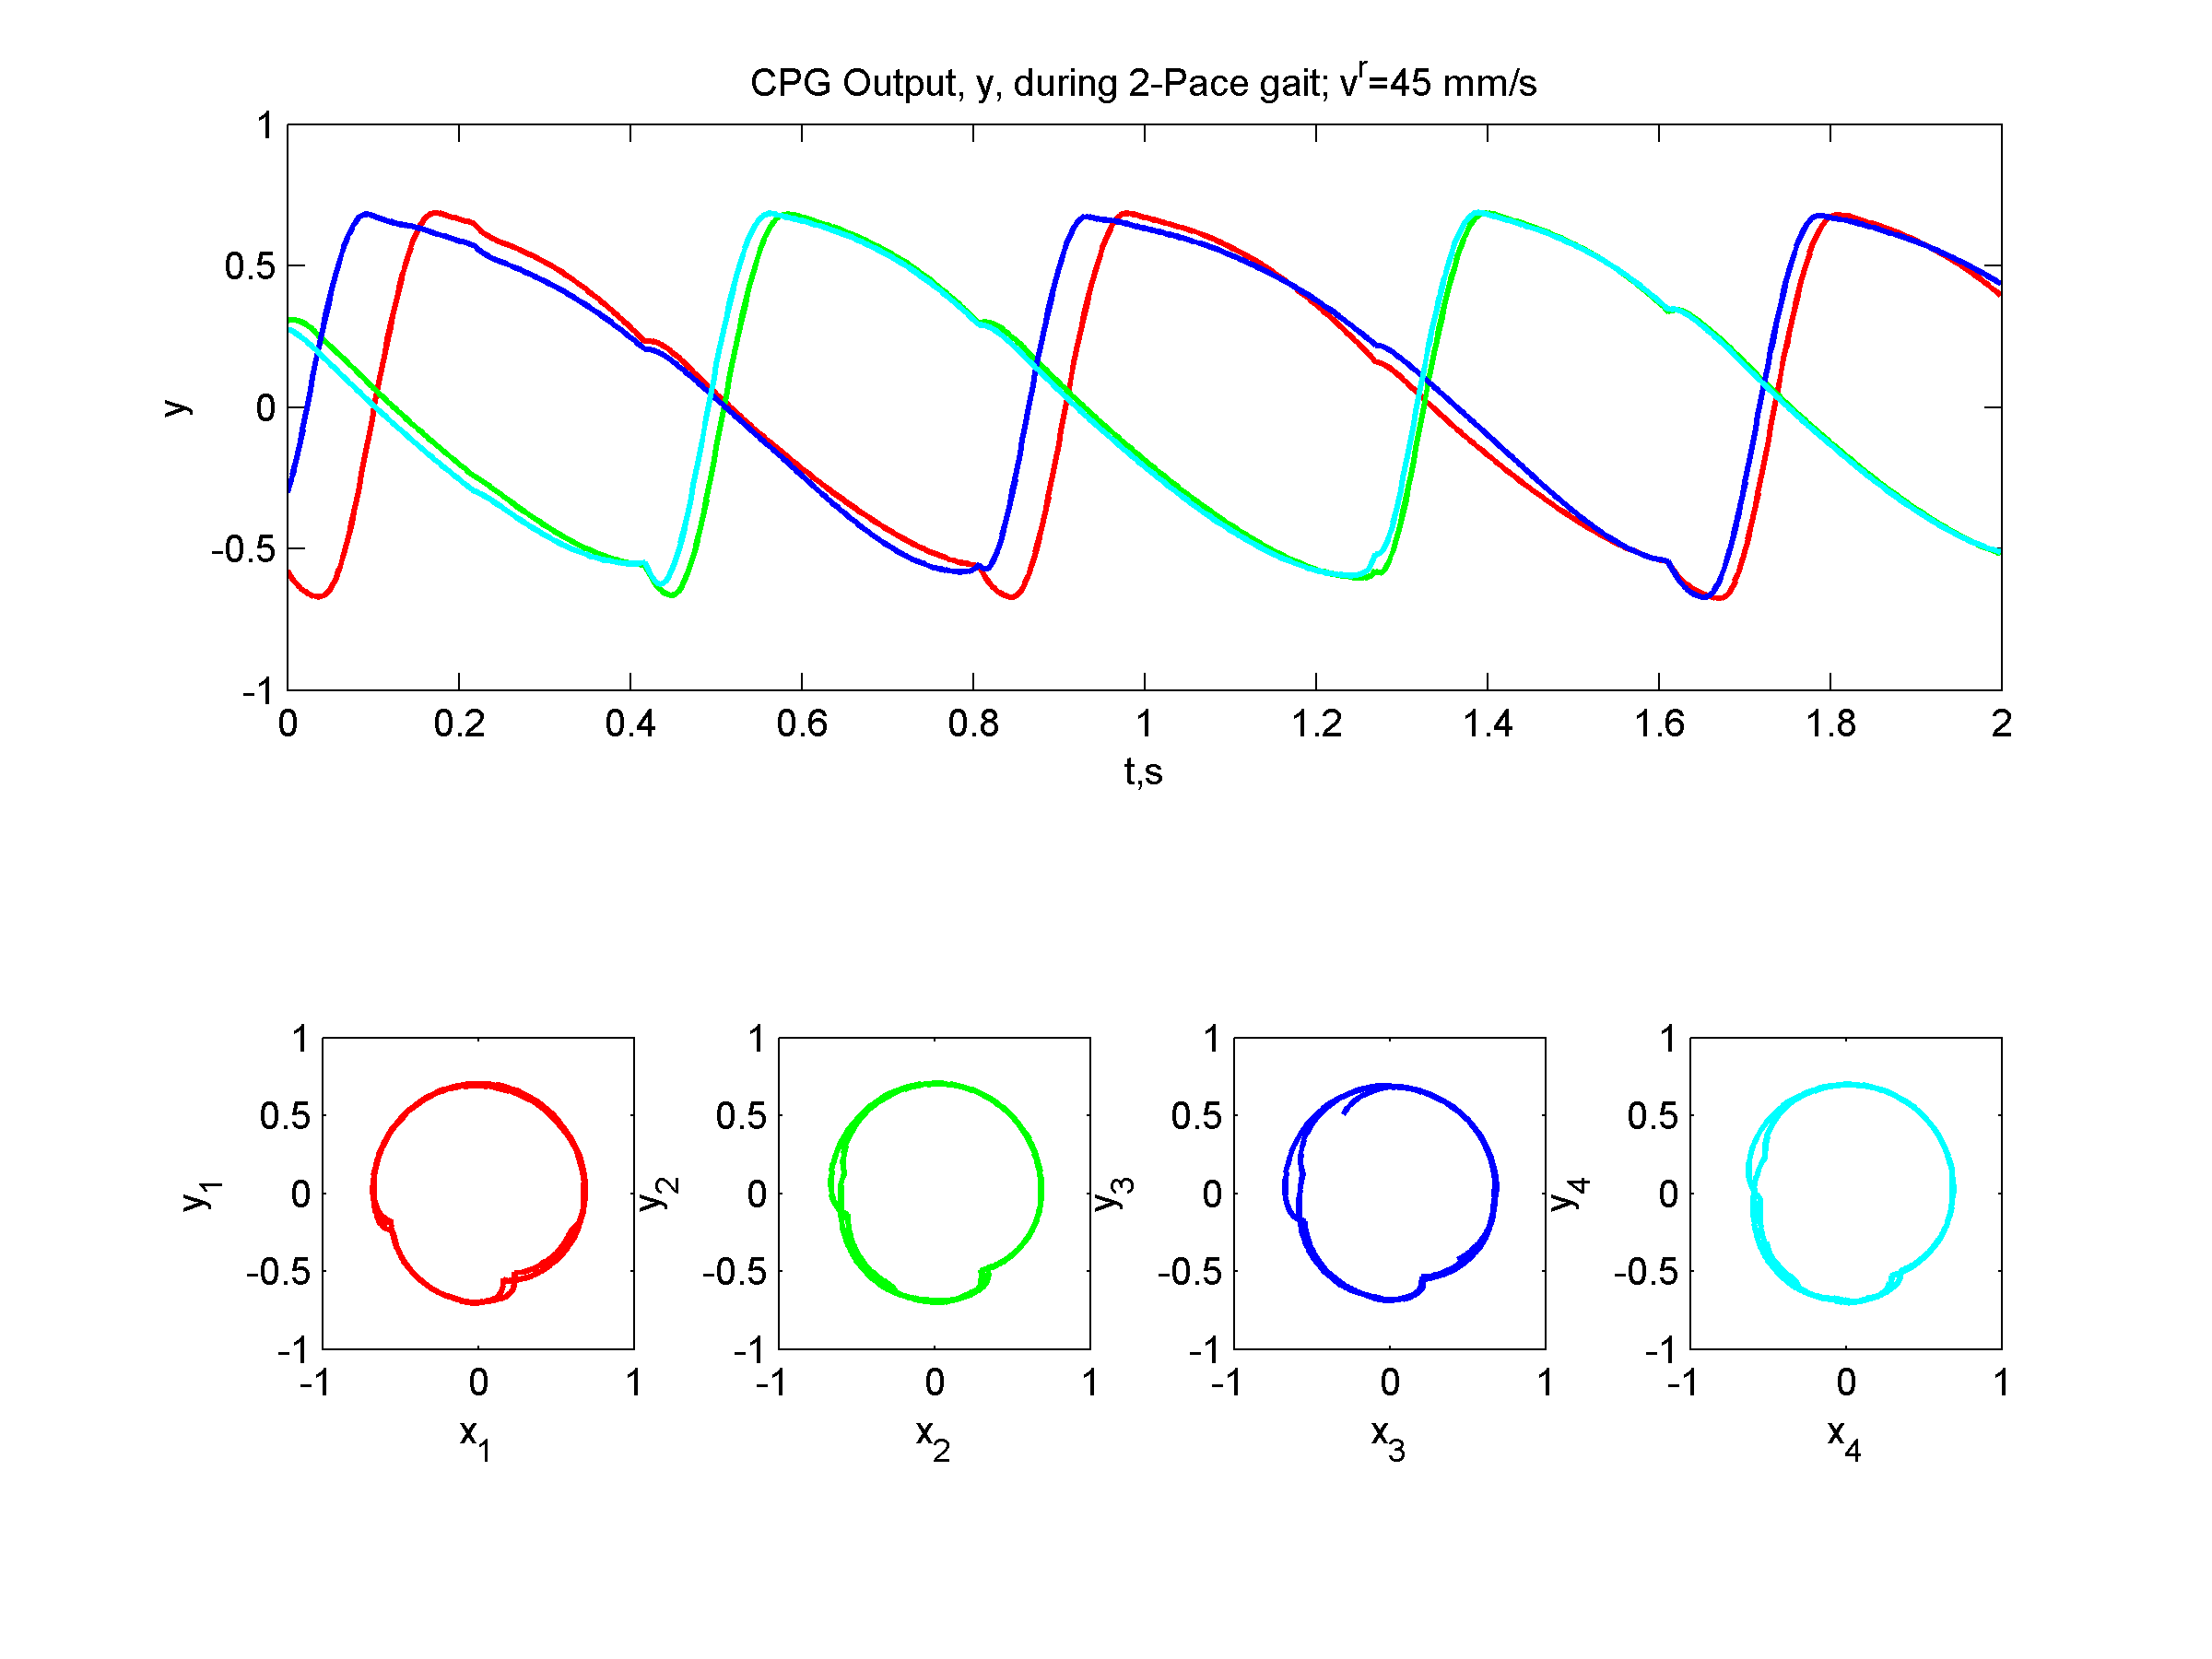
\includegraphics[width=1.00\textwidth]{cpg_phase2_45.png}}
				\caption{CPG output and phase plots for a two-paced gait over two gait cycles.}
				\label{fig::cpg_phase2_45}
			\end{figure}
			\begin{figure}[h!]
				\centering
				\fbox{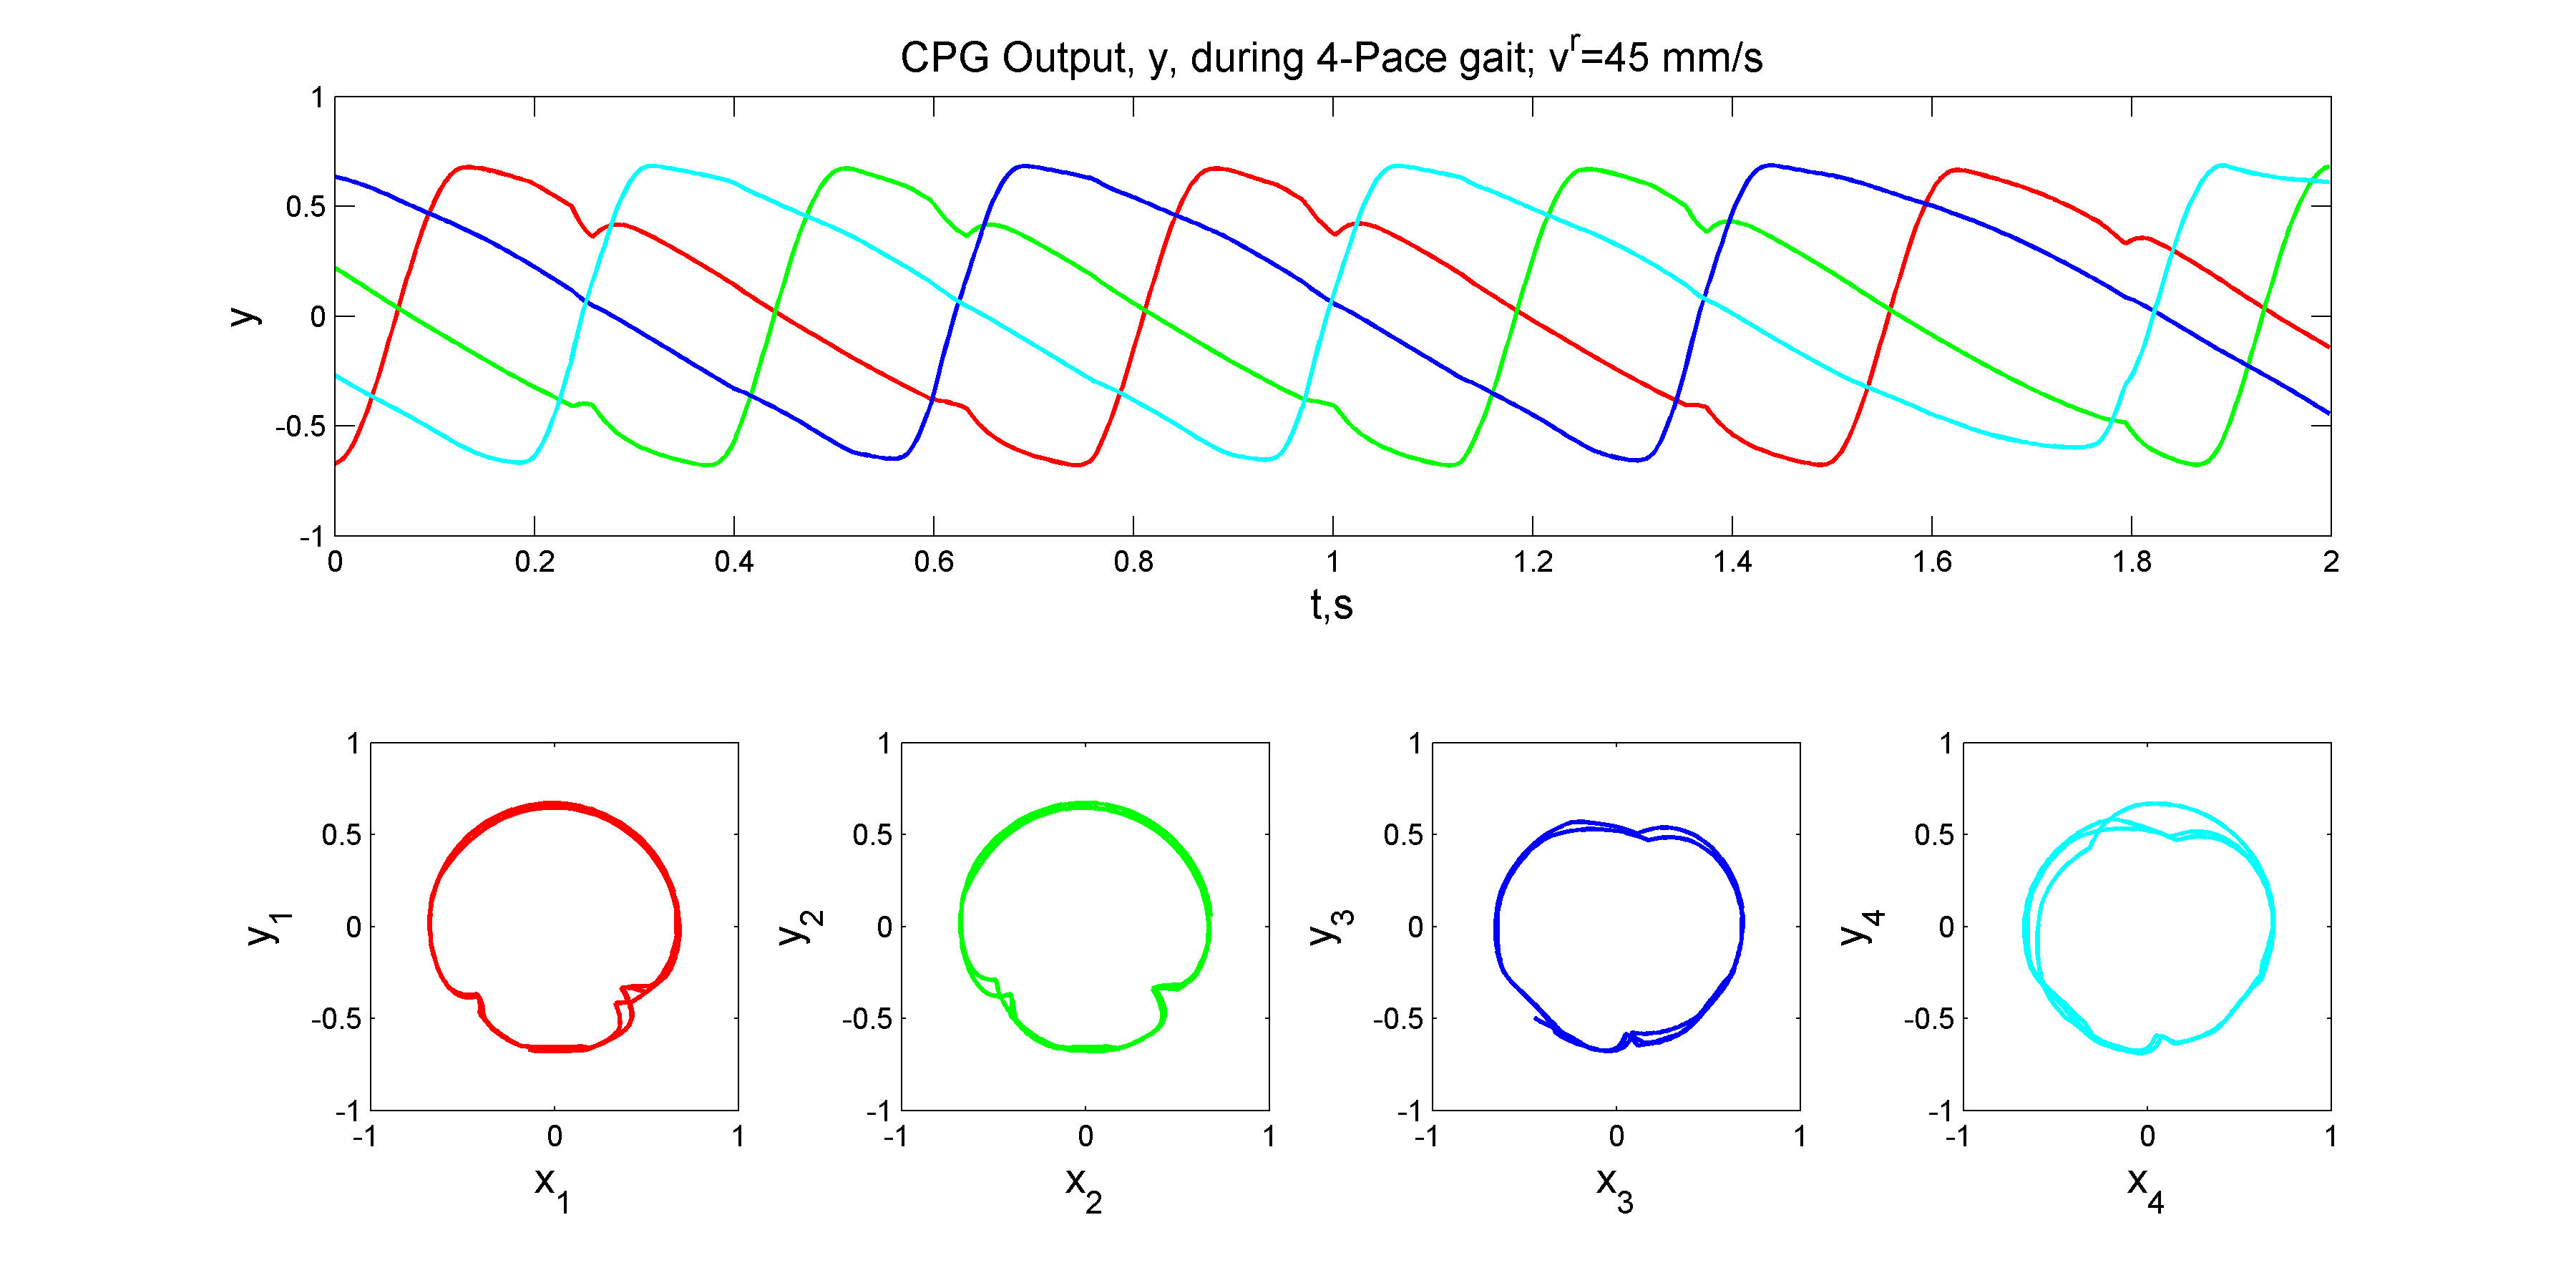
\includegraphics[width=1.00\textwidth]{cpg_phase4_45.png}}
				\caption{CPG output and phase plots for a two-paced gait over two gait cycles.}
				\label{fig::cpg_phase4_45}
			\end{figure}
			\begin{figure}[h!]
				\centering
				\fbox{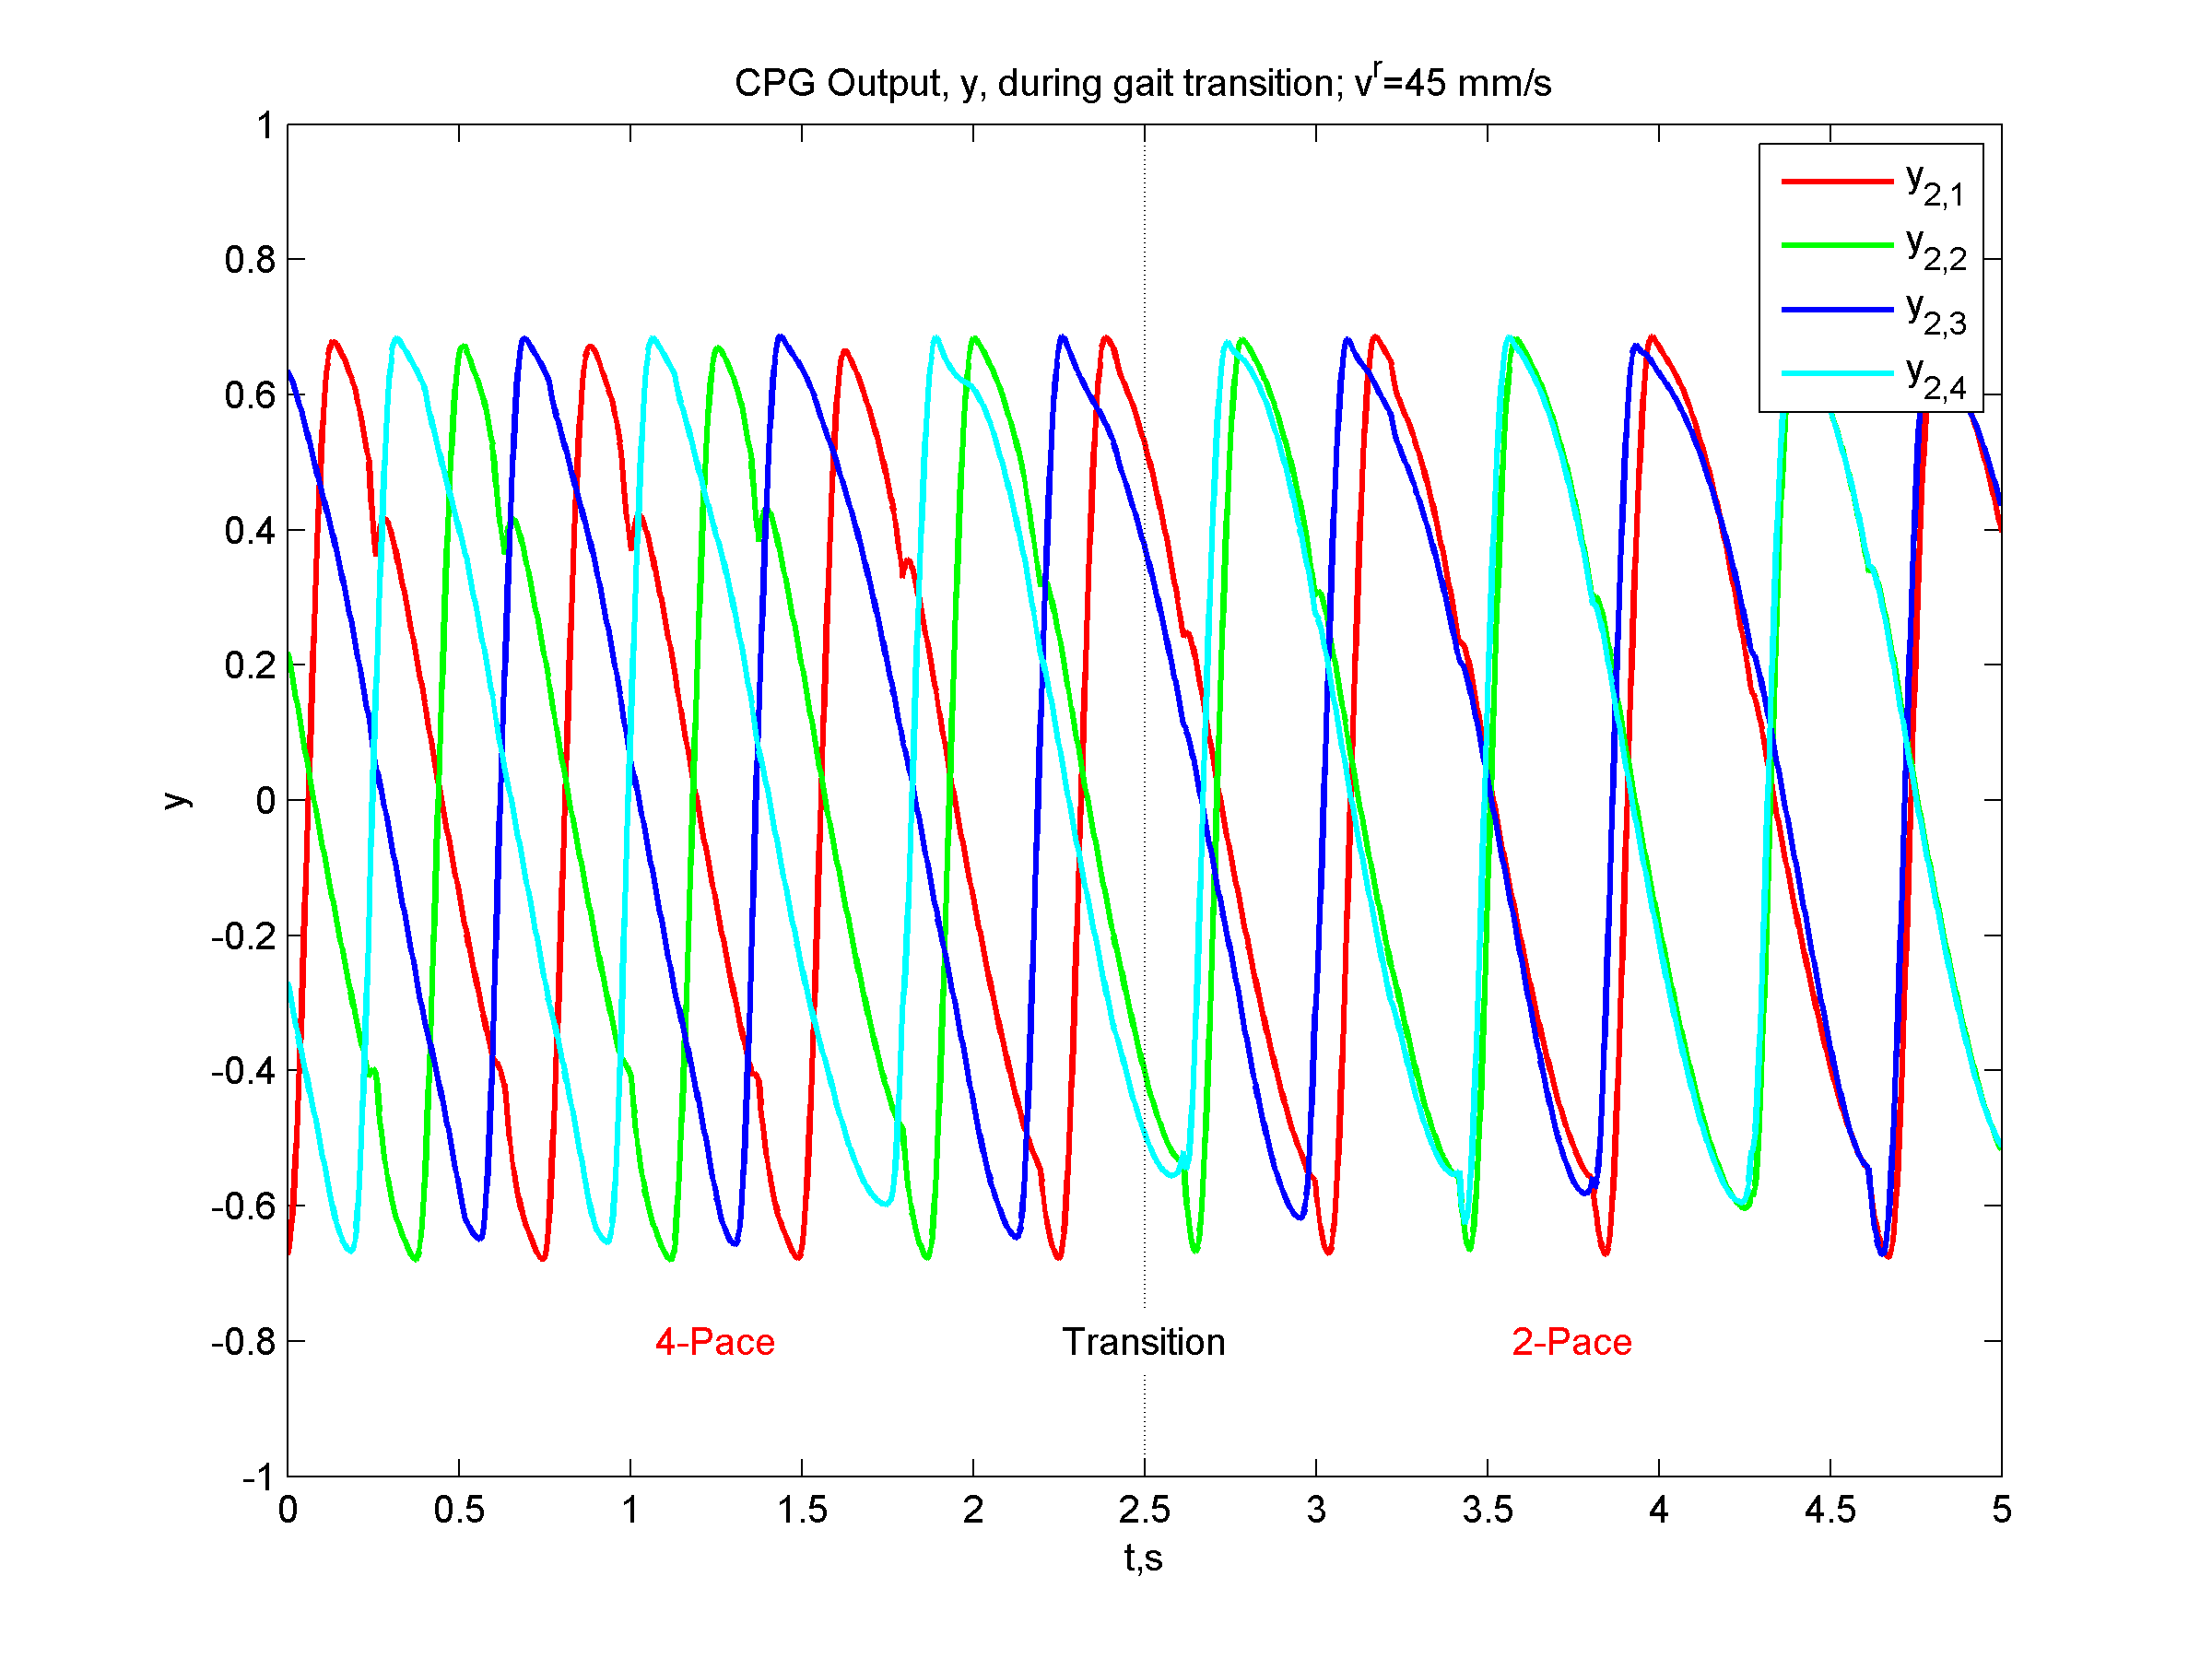
\includegraphics[width=1.00\textwidth]{cpg_transition.png}}
				\caption{CPG output transition during four-pace to two-pace gait switch.}
				\label{fig::cpg_transition}
			\end{figure}	%%%%%%%%%%%%%%%%%%%%%%%%%%%%%%%%%%%%%%%%%%%%%%%%%%%%%%%%%%%%%%%%%%%%%%%%%%



	\section{Foot Placement Control}


		A foot placement controller has been implemented which utilizes CPG outputs (defined in equation \ref{eq::cpg_ss_def}) in concert with a virtual-force controller. This controller is designed such that each foothold of the robot tracks the foot positions of a virtual robot generated through a model reference. The virtual robot is described by the foot positions, $\tilde{p}_{i,e}$, a virtual reference configuration corresponding to the position, $\tilde{p}_{c}$, and orientation, $\tilde{\theta}_{c}$, of the main body in $O_{0}$. The robot follows the foot placement of the virtual robot to achieve a commanded ground velocity $v^{r} \InRe{3} $; and turning velocity $\omega^{r} \InRe{}$. Each virtual point is updated by:
		\begin{eqnarray}
			\dot{\tilde{\theta}}_{c}	& = & \omega^{r} 	\nonumber\\
			\dot{\tilde{p}}_{c}			& = & v^{r}			\nonumber\\
			\dot{\tilde{p}}_{i,e} 		& = & v^{r} + \Skew{\omega^{r}\vec{h}_P} \tilde{R}_{P} \wrap{\tilde{p}_{i,e}-\tilde{p}_{c} } 
			\label{eq::virtual_foothold_control}
		\end{eqnarray}
		where $\vec{h}_P$ is a unit vector that is orthogonal and pointed outward from the surface beneath the robot and $\Skew{\omega^{r}\vec{h}_P}\text{ }\in \Real^{3\times3}$ forms a skew-symmetric matrix from the vector argument $\omega^{r}\vec{h}_P$. The virtual foothold dynamics progress the target footholds at a commanded translational (forward) and rotational velocity, $v^{r}$ and $\omega^{r}$, respectively. The robot follows the virtual model at nearly the same velocities with minimal lag so long as system bandwidth is not exceeded. Using this virtual-foothold method is convenient as it allows for foot-placement planning to be independent of foot-trajectory planning. For example, terrain adaptation can be incorporated by modifying the location of virtual foot positions such that they conform to an upcoming surface. The robot's gait will then track these adaptations without any explicit modification of foot trajectories. In the event of contact with unperceived terrain, virtual-foothold positions will reset with respect to the position of the contact.
%
			\begin{figure}[h!]
				\centering
				\fbox{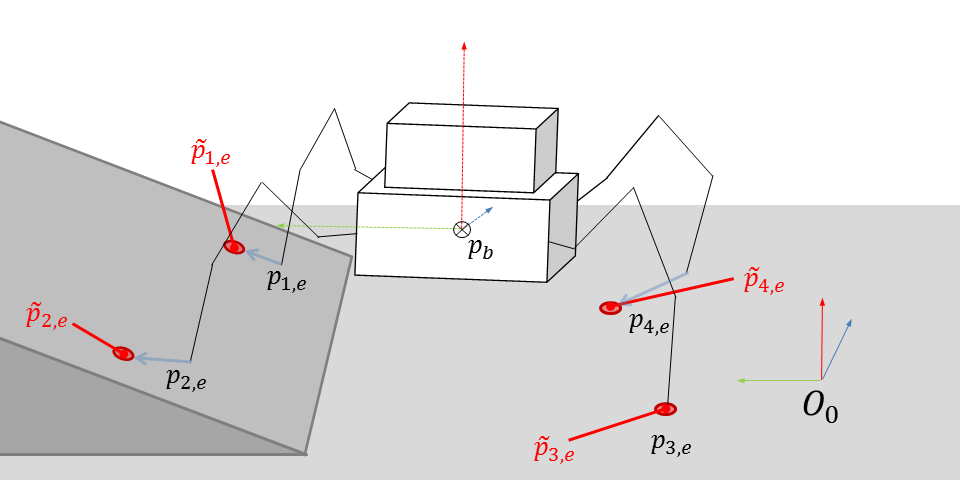
\includegraphics[width=0.75\textwidth]{virtual_foothold.png}}
				\caption{ Virtual foothold representation. Blue arrows represent an attractive ``force" between the feet and their corresponding virtual foothold.}
				\label{fig::virtial_foothold}
			\end{figure}
%
		The full foothold controller represented by 
			\begin{equation}
				\dot{p}_{i,e} = \dot{\tilde{p}}_{i,e}^{v} + \dot{\tilde{p}}_{i,e}^{y}, \SSep i = 1,...,4
			\end{equation} 
		is a composite of a foot-repositioning and step-height controller which are formulated in terms of the dynamics of the signals $\dot{\tilde{p}}_{i,e}^{v}$ and $\dot{\tilde{p}}_{i,e}^{y}$, respectively. Each foot is treated as a point mass attracted to their corresponding virtual foothold by an over-damped mass-attractor system. $\dot{\tilde{p}}_{i,e}^{v}$ is defined by
			\begin{equation}
				\label{eq::FootControl}
				\dot{\tilde{p}}_{i,e}^{v} 		= \frac{1}{m_{i}} \int^t{{P}_{\vec{h}_{i}} \wrap{ F_{s,i}  -b_{c} \dot{p}_{i,e} + F_{\epsilon,i} } d\tau}
			\end{equation}
		where
			\begin{eqnarray*}
				F_{s,i} 			& = & k_{c}  \mu_{i} \wrap{ \tilde{p}_{i} - {p}_{i,e} } \Unit{y_{2,i}}		\nonumber\\
				F_{\epsilon,i}		& = & a_{\epsilon}\dot{\epsilon}_{\theta} \Unit{y_{2,i}}						\nonumber
			\end{eqnarray*}
	 	with $k_{c},b_{c},a_{\epsilon},m_{i} \InRe{}$.
		$k_{c}$ and $b_{c}$ represent  attraction and viscous damping constants for the virtual force system. ${P}_{\vec{h}_{i}}(*)$ projects the sum of  forces, $(*)$, onto the surface beneath the \Ith foot orthogonal to $\vec{h}_{i}$. $\Unit{y_{2,i}}$ is a standard unit step function. The force $F_{\epsilon,i}$ is a compensatory force to adjust for the inertial disturbance,  $\dot{\epsilon}_{\theta}$. For instance, if the robot was pushed from the side of its body, this force would induce a side stepping motion in attempt to compensate for the disturbance. Because of $\Unit{y_{2,i}}$, $F_{s,i}$ and $F_{\epsilon,i}$ are nonzero only when $y_{2,i}$ is positive.

		The controller component $\dot{\tilde{p}}_{i,e}^{y}$ is defined from the CPG output signal $\dot{y}_{2,i}$. The height of each step is made proportional to the magnitude of desired platform velocity.
		\begin{equation}
			\dot{\tilde{p}}_{i,e}^{y} 	= { \wrap{ \alpha_{v} v^{r}+\alpha_{\omega} \omega^{r} } \dot{y}_{2,i}} \vec{h}_{i} 
			\label{eq::FootControl}
		\end{equation}
		where $\alpha_{v}$ and $\alpha_{\omega}$ are scalar weighting parameters. Scaling step height relative to command parameters $v^{r}$ and $\omega^{r}$ has been seen in experimental studies to be more effective than using a fixed step-height for all gait configurations. Figures \ref{fig::foot_motion2} and \ref{fig::foot_motion4} shown foot motion patterns using the aggregate virtual-force foothold controller and CPG motion outputs during two and four-paced gaits, respectively, which achieve a forward velocity of $v^{r}=60\frac{mm}{s}$, .
%
			\begin{figure}[h!]
				\centering
				%\fbox{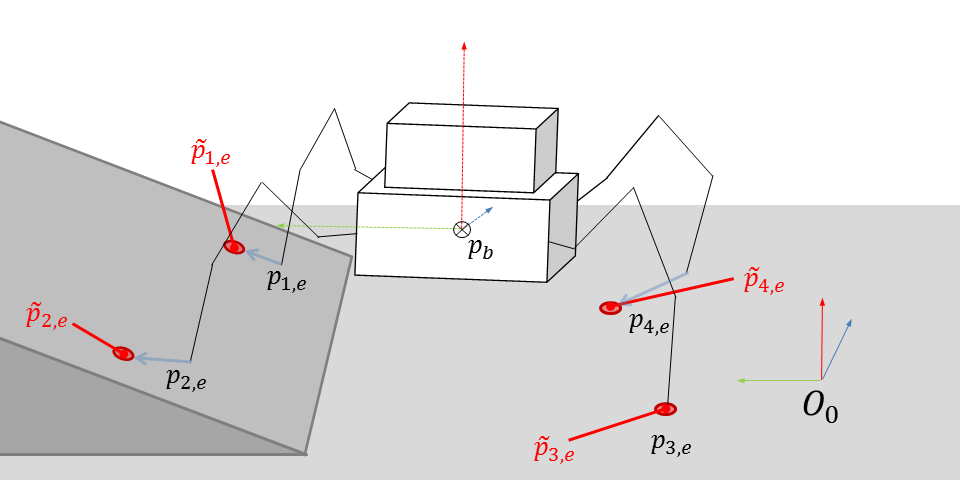
\includegraphics[width=0.75\textwidth]{virtual_foothold.png}}
				\caption{Foot motion generated using virtual-force foothold controller during two-pace gait sequence at $v^{r}=60\frac{mm}{s}$.}
				\label{fig::foot_motion2}
			\end{figure}
			\begin{figure}[h!]
				\centering
				%\fbox{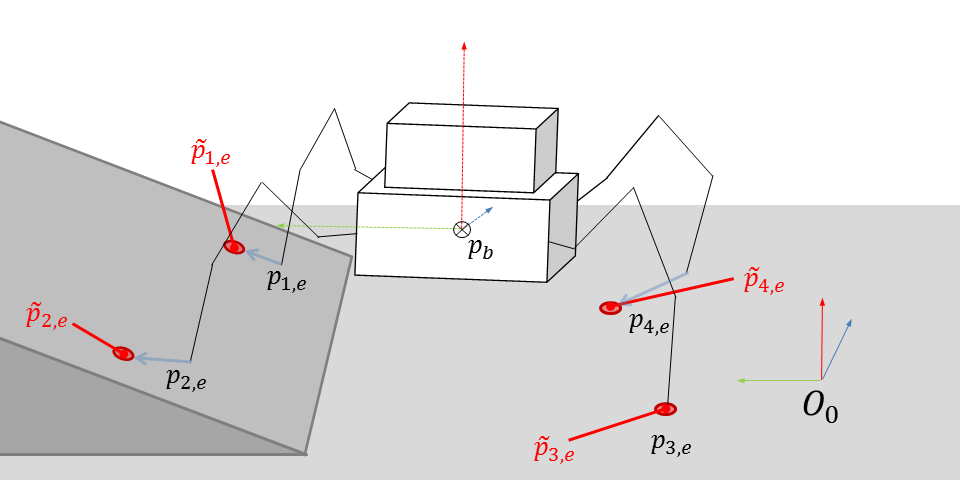
\includegraphics[width=0.75\textwidth]{virtual_foothold.png}}
				\caption{Foot motion generated using virtual-force foothold controller during two-pace gait sequence at $v^{r}=60\frac{mm}{s}$.}
				\label{fig::foot_motion4}
			\end{figure}
%



	\section{ZMP Based Trunk-Placement Control}

		A  modified Zero-Moment-Point (ZMP) based controller is utilized in positioning BlueFoot's body during gaiting. In this context, the ZMP of the system is a set of state values for which the net-torque exerted upon the system, about the COG, is zero \cite{Kajita2003,Katie2009}. Unlike \cite{Takanishi1989,Kurazume2003}, which address ZMP-based control by considering the robot's body as point-mass with massless limbs, this method takes into account the torque contribution of each non-supporting leg. Each leg in flight is considered as a series of point masses whose locations are computed using joint position feedback and trunk orientation estimates, in concert with robot's forward kinematic model.
		
		The ZMP approach is used to first calculate static ZMP configurations ( \IE $\ddot{p}_{COG}\approx0$) at each time instance. The distance between the robot's COG and associated ZMP is incrementally minimized on-line by treating the ZMP as a  mass-attractor and ``pulling" a reference body position, ${p}_{b}^{b',r}$, towards the ZMP point at each update. This differs from approaches similar to \cite{Kurazume2003} because these routines feature off-line, trunk trajectory design which aim to minimize deviations between the robot's COG and ZMP by creating an appropriate limit-cycle motion for the robot's trunk. These approaches typically utilize simplified, linearized models of the actual system about marginally-stable equilibrium points. To realize an adjustment of the robot's COG, towards the ZMP, BlueFoot's trunk position is modified during the execution of a gait. The trunk is controlled (and not individual feet) as it contributes most of the system's total mass and, thus, has the greatest influence over the location of the platform's COG. Restricting adjustments to the trunks translational states allow pre-planned foot trajectories to remain unmodified by the ZMP-control module during gait execution, thus decoupling foot-placement and body-placement control.

		To incrementally compute the static ZMP of the platform, a measure of net-moment on the body of the platform must be known. The net-moment due to gravitational forces, $\tau_{net}$, is approximated using the locations of each link and joints as point-mass loads. Hence, $\tau_{net}$ is calculated as follows:
			\begin{equation}
				\tau_{net} 	=  \wrap{\bar{p}_{b}^{b'}-\hat{p}_{COG}^{b'} } \times \wrap{\vec{g} m_{b}}	+ \tau_{legs}
				\label{eq::net_moment}
			\end{equation}
		where
			\begin{eqnarray*}
					\tau_{legs}		& = & \Sum{i}{1}{4} (1-\mu_{i})  \Sum{i}{1}{4}   \wrap{ m_{i,j}^{J} d_{i,j}^{J} + m_{i,j}^{L} d_{i,j}^{L} }	\times \vec{g} \nonumber \\
					d_{i,j}^{J} 	& = & {{p}_{i,j}^{b'}-\hat{p}_{COG}^{b'}.} \nonumber \\														
					d_{i,j}^{L} 	& = &
					\begin{cases}
					{ 0.5  \wrap{{p}_{i,j+1}^{b'}-{p}_{i,j}^{b'}} + {p}_{i,j}^{b'} - \hat{p}_{COG}^{b'}} 	&\text{if } j < 4 \\
					{ 0.5  \wrap{{p}_{i,e}^{b'}-{p}_{i,j}^{b'}} + {p}_{i,j}^{b'} - \hat{p}_{COG}^{b'}} 		&\text{if } j = 4
					\end{cases} \nonumber
				\label{eq::Levers}
			\end{eqnarray*}
		with $m_{b}$, $m_{i,j}^{J}$ and $m_{i,j}^{L}$ represent the mass of the main body; the mass of each joint; and the mass of each link, respectively. $\mu_{i}$ is included in the above formulation such that only stepping legs contribute to  $\tau_{legs}$. It should be noted that the superscript ${b'}$ denotes that each particle considered in this controller is defined with respect to the robot-relative frame $O_{b'}$ define in Section \ref{sec::system_kinematics}. This allows the control routine to be performed without explicit knowledge of the system in space. The estimated center of gravity in $O_{b'}$, $\hat{p}_{COG}^{b'}$, is generated as follows:
			\begin{eqnarray*}
				\hat{p}_{COG}^{b'} 	& = & \frac{1}{m_{T}}\wrap{ m_{b}p_{b}^{b'} + \sum_{i=1}^{4} \wrap{m_{i,e}{p}_{i,e}^{b'} + \sum_{j=1}^{4} \wrap{  m_{i,j}^{J}{p}_{i,j}^{b'} +  m_{i,j}^{L}{p}_{i,j}^{b',L} } }} 	\nonumber \\
				{p}_{i,j}^{L} 	& = & 
					\begin{cases}
					{ 0.5  \wrap{{p}_{i,j+1}^{b'}-{p}_{i,j}^{b'}} + {p}_{i,j}^{b'} } 	&\text{if } j < 4 \\
					{ 0.5  \wrap{{p}_{i,e}^{b'}-{p}_{i,j}^{b'}} + {p}_{i,j}^{b'} } 		&\text{if } j = 4
					\end{cases} \nonumber
				\label{eq::cog_estimate}
			\end{eqnarray*}
		where
			\begin{equation}
				m_{T} = m_{b} + \sum_{i=1}^{4} \wrap{m_{i,e} + \sum_{j=1}^{4} \wrap{  m_{i,j}^{J} +  m_{i,j}^{L} } }
			\end{equation}

		Setting $\tau_{net}=0$, \ref{eq::net_moment} is manipulated to a derived solution for the ZMP as follows:
			\begin{equation}
				{p}_{ZMP}^{b'} = R_{z_P} \wrap{\frac{\pi}{2}}  \wrap{ \frac{\norm{g}}{m_{b}}} \tau_{legs} + \hat{p}_{COG}^{b'}.
				\label{eq::ZMPFromMoment}
			\end{equation}
		Using ${p}_{ZMP}^{b'}$, the platform's posture is then updated using a virtual-force controller. Moreover, ${p}_{b}^{b'}$ is to be controlled through  ${p}_{b}^{r}$ such that it is smoothly attracted to ${p}_{ZMP}$. The controller is given by
			\begin{equation}
				\dot{p}_{b}^{r} 	= {P}_{\vec{h}_{i}} \wrap{K_{Z}	( {p}_{ZMP}^{b'} - {p}_{b}^{b'} )  
				+ K_{F}\frac{F_{r}}{m_{b}}  }
				\label{eq::ZMPController}
			\end{equation}	
		where
			\begin{eqnarray*}
				F_{r} 	& = &  \Sum{i}{1}{4}  e^{\wrap{ k_{l} r_{i}^{-} } } + e^{ \wrap{ k_{l} r_{i}^{+} } } \nonumber \\
				r_{i}^{+}	& = & \norm{{p}_{i,e}^{b'}- {p}_{b}^{b'}} - r_{max} \nonumber \\
				r_{i}^{-}	& = & r_{min} - \norm{{p}_{i,e}^{b'}- {p}_{b}^{b'}} \nonumber
			\end{eqnarray*}
		and $K_{Z}, K_{F}, K_{c}, K_{\epsilon}, k_{l} > 0$ and $\dot{p}_{b}^{b',r}$ is the reference body velocity. $F_{r}$ is a boundary force added to ensure that the workspace of each manipulator, defined by the radii $r_{min}$ and $r_{max}$, is not exceeded when the body is repositioned. $k_{l}$ is picked to be adequately large such that this force is nearly zero when the body and foot positions comply with the local workspace of each leg, and large when the workspace is nearly compromised, forcing the placement of the body to comply with each leg workspace. Figure \ref{fig::body_motion} shows trunk reference trajectory, ${p}_{b}^{b',r}$ and actual body trajectory, ${p}_{b}^{b'}$ generated using the aforementioned ZMP-based body-placement controller during a gait which achieves a forward velocity of $v^{r}=60\frac{mm}{s}$.
			\begin{figure}[h!]
				\centering
				%\fbox{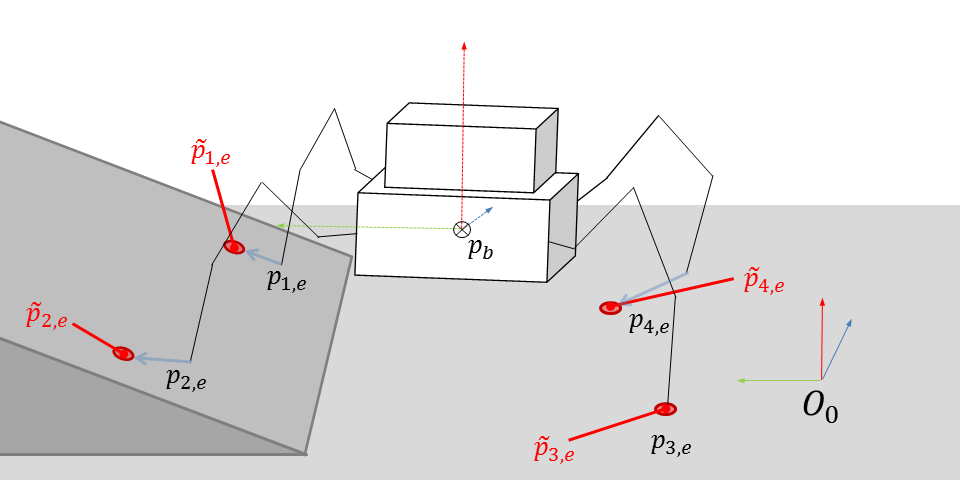
\includegraphics[width=0.75\textwidth]{virtual_foothold.png}}
				\caption{Foot motion generated using virtual-force foothold controlle.}
				\label{fig::body_motion}
			\end{figure}
%




	\section{Trunk Leveling via NARX-Network Learning Approach}

		Suppressing disturbances which enter a quadruped system during gaiting is a matter which requires special handling, given the the general dynamical complexity of both the robot and its interactions with the its environment. This complexity can be handled, in part, by a learning-based approach. This section will focus on the formulation of a learning controller used to reject disturbances from the orientation states of the trunk of a legged robot. Disturbance rejection from the trunk sub-system of a legged platform has practical significance when carrying a payload (such as cameras, optical systems, armaments, etc.) rigidly fixed to their main body. Disturbances are imparted upon the trunk during gaiting in two main ways: 
		\begin{enumerate}
			\item instantaneous changes in force distribution when feet make and break contact with the ground 
			\item under-actuation that occurs during certain dynamic gaits. During dynamic gaits, such as trot gaits, the state of contact between the feet and the ground is changed often so as to prevent the walking robot from tipping past a recoverable configuration. 
			\end{enumerate}
		Additionally, these gaits feature the utilization of two or fewer legs to support the trunk at any given time, causing the system to enter an under-actuated state where the body is free to rock about the planted feet, as shown in Figure \ref{fig::quadruped_walking}.
		%%
			\begin{figure}[h!]
			\centering
				\fbox{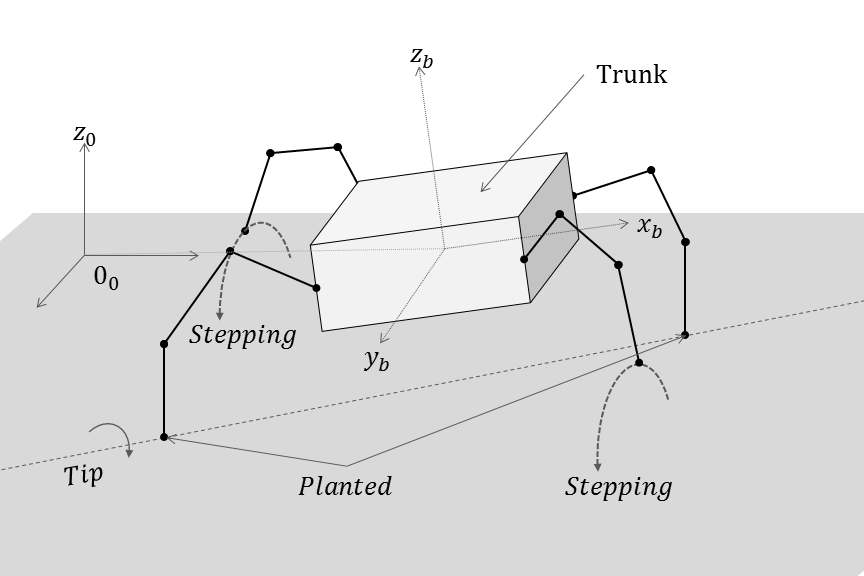
\includegraphics[width=0.80\textwidth]{tipping_robot.png}}
				\caption{ Quadruped tipping about planted feet. }
				\label{fig::quadruped_walking}
			\end{figure}
		%%
		To achieve disturbance rejection on the trunk orientation and to attain a fixed orientation, experimentation has been performed using a control methodology which utilizes a Nonlinear Autoregressive Neural Network with Exogenous inputs (NARX-NN) as part of an active compensation mechanism. The network is used to estimate the system dynamics and, further, predict periodic disturbances in an on-line fashion. The compensator is utilized to modify referential joint trajectories by way of a weighted sum between the original joint trajectories generated by the gaiting mechanism and a reference correction signal generated by the compensator.

		\subsection{NARX-Neural Network}


			Using a NARX-NN (introduced in Chapter \ref{ch::introduction}), the dynamical estimate $\hat{\Phi}_{k}$ is generated as a prediction of the sampled system dynamics, $\hat{\psi}_{k+1}$. The relationship between $\hat{\Phi}_{k}$ and the network prediction $\hat{\psi}_{k+1}$will be made clear in the description of the network training signal given in \ref{eq::training_signal}. The general input-output relationship of the NARX-NN predictor, $\emph{N}$, is described as follows:
			%%%
			%%%
				\begin{eqnarray}
					\hat{\psi}_{k+1}	&=& \emph{N}(\hat{\Psi}_{k}^{N},{U}_{k}^{N}) \nonumber\\
					\hat{\Psi}_{k}^{N}	&=& [\hat{\psi}_{k},\hat{\psi}_{k-1},...,\hat{\psi}_{k-N+1}]  \nonumber\\
					{U}_{k}^{N}		&=& [u_{k}   ,u_{k-1}   ,...,u_{k-N+1}   ]
					\label{eq::narx_model}
				\end{eqnarray}
			%%%
			%%%
			where ${U}_{k}^{N}$  and $\hat{\Psi}_{k}^{N}$ are collections of $N$ most recent samples of the network inputs, $u_{k}$, and the network output, $\hat{\psi}_{k}$, respectively. The NARX-NN input, $u_{k}$, represents a tuple $u_{k} = (z_{1,k}, z_{2,k}, f_{ext,k})$ whose components are the arguments of $\Phi$ at time instant $k$. 



		\subsection{NARX-NN Training Regimen}
			
			The  NARX-NN training signal is formulated to estimate $\Phi_{k}$ from the system dynamics. By \ref{eq::sampled_dynamics}, it can be seen that $\Phi_{k}$ can be estimated if ${z}_{2,k+1}$ can be predicted. We consider the following target network prediction output, $\psi_{k+1}$,  defined by:
				\begin{equation}
					\psi_{k+1} = \tau_{k} - \hat{M}_{1,k}({z}_{2,k+1} - {z}_{2,k})\Delta_{s}^{-1} = \Phi_{k} - {e}_{2,k}^{\Delta_{s}} \text{ .}
					\label{eq::training_signal}
				\end{equation}
			%%
			%%
			This training signal formulation assumes that $\hat{M}_{1,k}$ represents $M_{1,k}$ exactly, which is likely not the case given the system's complexity. In the absence of a well-modeled $\hat{M}_{1,k}$, a constant symmetric $\hat{M}_{nom}$ will be picked such that $\hat{M}_{1,k} = \hat{M}_{nom} \forall k$. $\hat{M}_{nom}$ has the following structure:
				\begin{equation}
					\hat{M}_{nom} = \left[
						\begin{array}{cc}
						\hat{M}_{bb}	&	 \hat{M}_{bq}\\
						\hat{M}_{qb}	&	 \hat{M}_{qq}
						\end{array}
					\right]
				\end{equation}
			where 	$\hat{M}_{bb}\RealMat{6}{6}$, 
					$\hat{M}_{bq}=\hat{M}_{qb}^{T} \RealMat{6}{16}$, and  
					$\hat{M}_{qq}\RealMat{16}{16}$. 
			It is particularly important that $\hat{M}_{bq}\neq0$ to reflect some degree of coupling between the joint states $q$ and the trunk states ${p}_{b}$ and $\theta_{b}$. In general, if $\hat{M}_{nom}$ should be selected to reflect the \emph{average} system mass matrix over the range of configurations, $z_{1}$, seen during gaiting. This approximation has shown to be adequate from our results, and depends on the assumption that changes in $\hat{M}_{1,k}$ are small  over the subset of state $z_{1}$ experiences during a periodic gaiting sequence. Future improvements of this controller involve the formulation of a separate estimator for $M(z_{1})$, or a control/learning scheme with no direct dependence on $M(z_{1})$.

			Since $\hat{\psi}_{k+1}$ is non-causal, training is performed one time-step after a prediction is made using the input-output pair $\hat{\psi}_{k}$ and \{${\Psi}_{k-1}^{N}$, ${U}_{k-1}^{N}$\}. Note that $\hat{\psi}_{k}$ can calculated directly using \ref{eq::training_signal} where all component signals are time-delayed by one time-step. Training can then be described by:
				\begin{equation}
					\psi_{k} \xrightarrow{BP(\gamma^{lr})} \emph{N}({\Psi}_{k-1}^{N},{U}_{k-1}^{N})
					\label{eq::training}
				\end{equation}
			where $\gamma^{lr} _{min} < \gamma^{lr} < \gamma^{lr} _{max}$ is a learning rate adapted using a \emph{bold-driver} update routine. Bold-driver learning-rate adaptation is a  heuristic method for speeding up the rate of convergence of back-propagation training regimes \cite{Battiti1992,Magoulas1999}. This $\gamma^{lr}$ update law is parameterized by $\beta \in (0,1)$ and $\zeta \in (0,1)$ which are selected to specify the amount by which $\gamma^{lr}$ increases or decreases per update, and $\gamma^{lr} _{min}$ and $\gamma^{lr} _{max}$ which are used to saturate $\gamma^{lr}$.  The bold-driver scheme utilizes the current and previous mean-squared network output error values ($MSE_{k}$ and $MSE_{k-1}$, respectively) to adjust $\gamma^{lr}$ as follows:
				\begin{equation}
				    \gamma^{lr} \leftarrow 
					\begin{cases}
				    \gamma^{lr} (1- \beta) 		& \text{if } MSE_{k} > MSE_{k-1}\\
				    \gamma^{lr} (1+\zeta \beta),& \text{otherwise}.
					\end{cases}
				\end{equation}
			Since network training is being performed on-line as an incremental routine, the effective mean-squared NARX-NN  output error is low-passed by a factor $\lambda \in (0,1)$. This update technique has been selected to ensure that outliers presented during training do not affect network learning updates as significantly as ``nominal" training pairs. Network output error, $e_{\emph{N},k}$, and its associated MSE values are calculated after each prediction by:
				\begin{eqnarray}
					e_{\emph{N},k} 	&=& \hat{\psi}_{k} - \psi_{k} \nonumber\\
					MSE_{k} 		&\leftarrow& \lambda \|e_{\emph{N},k}\|_{2}^{2} + MSE_{k-1}(1-\lambda).
				\end{eqnarray}


		\subsection{Compensator Output}

			The control scheme is first presented with respect to the servo input torques, $\tau_{q,k}$, and formulated to achieve a level trunk characterized by $\theta_{b}=0$, $\dot{\theta}_{b}= 0$. To formulate this controller, the dynamical sub-system which corresponds to the un-actuated trunk orientation states is isolated by:
				\begin{equation}
					\ddot{\theta}_{b} 	= \Gamma_{1} M^{-1}(z_{1})( \Gamma_{2}\tau_{q}	 + \Phi)
					\label{eq::sub_dynamics}
				\end{equation}
			where 
				\begin{eqnarray*}
					\Gamma_{1} &=& [0_{3\times3},I_{3\times3},0_{3\times16}] \nonumber\\
					\Gamma_{2} &=& [0_{16\times6},I_{16\times16}]^{T}	
				\end{eqnarray*}
			and $\Gamma_{2}\tau_{q}$ is equivalent to the original system input, $\tau$. In order to enforce a level platform with zero angular velocity, we seek a $\tau_{q}$ which emulates the proportional-derivative (P.D.) control law:
				\begin{equation}
				 	\ddot{\theta}_{b} = - K_{b}{\theta}_{b} - K_{d}\dot{\theta}_{b}
				\end{equation}
			where $K_{b}$ and $K_{d}$ are constant gain matrices. Using this P.D. law and \ref{eq::sub_dynamics}, we propose a least-squares solution for $\tau_{q}$ by:
				\begin{equation}
					\tau_{q} \approx -\left[\Gamma_{1} M^{-1}(z_{1}) \Gamma_{2}\right]^{\dagger}\Gamma_{1} M^{-1}(z_{1})(\Phi + K_{b}{\theta}_{b} + K_{d}\dot{\theta}_{b} )
					\label{eq::psuedo_torque}
				\end{equation}
			where $\left[*\right]^{\dagger}$ denotes the Penrose-Moore pseudo-inverse of $[*]$.
			%%
			Replacing all dynamical terms with their associated discrete-time equivalents, and $\Phi$ by the NARX-NN output $\hat{\Phi}_{k}=\hat{\psi}_{k+1}$, we apply \ref{eq::psuedo_torque} to arrive at the following required joint torque estimate:
				\begin{equation}
					\hat{\tau}_{q,k} =  -\left[\Gamma_{1} \hat{M}^{-1}_{1,k} \Gamma_{2}\right]^{\dagger} \Gamma_{1}\hat{M}^{-1}_{1,k}( \hat{\psi}_{k+1} + K_{b}{\theta}_{b,k} + K_{d}\dot{\theta}_{b,k} )
					\label{eq::psuedo_torque_k}
				\end{equation}
			where ${\theta}_{b,k}$ and $\dot{\theta}_{b,k}$ are samples of angular trunk position and rate, respectively.


			Using the joint controller dynamics presented in \ref{eq::servo_control_dynamics} and the estimate $\hat{\tau}_{q,k}$, we can formulate a reference-trajectory correction  which is used to alter the joint reference positions, ${q}_{k}^{r}$. Moreover, the corrected reference position, ${q}_{1,k}^{r,*}$ is generated such that the estimated output torque $\hat{\tau}_{q,k}$ is attained by each joint controller. This joint-reference compensator output is defined using 
			\ref{eq::psuedo_torque_k} as follows:
				\begin{equation}
				 	{q}_{1,k}^{r,*} 	= k_{s}^{-1}  \left(  \hat{\tau}_{q,k}  \right) +  {q}_{1,k}.
					\label{eq::correction_equation}
				\end{equation}
			The correction signal,  ${q}_{k}^{r,*}$, is combined with the original gaiting trajectory signal, ${q}_{k}^{r}$, as a weighted sum to form a compensated joint control reference signal, $\tilde{q}_{k}^{r}$, defined by:
				\begin{equation}
				 	\tilde{q}_{k}^{r} 	\leftarrow (1-\alpha) {q}_{k}^{r} + \alpha ( {q}_{k}^{r,*} )
					\label{eq::correction_application}
				\end{equation}
			where  $\alpha \in (0,1)$ is a uniform mixing parameter. The parameter $\alpha$ must be tuned with respect to the stability margins of the gait being compensated. The resultant $\tilde{q}_{k}^{r}$ is then applied  to each joint controller in place of the original reference signal,  ${q}_{k}^{r}$,  generated by the gait controller. Selection of the parameter $\alpha$ is crucial for achieving good performance. 

				\begin{figure}[h!]
					\centering
					\fbox{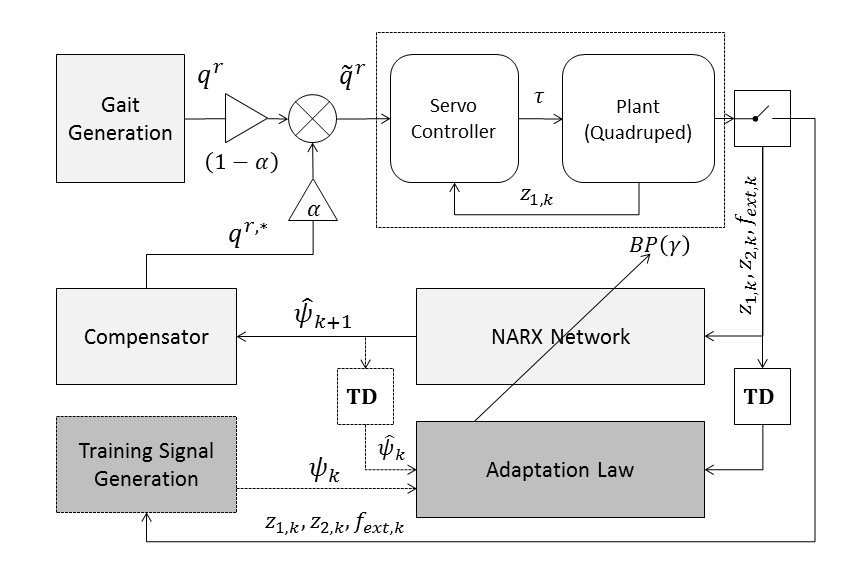
\includegraphics[width=1.00\textwidth]{controller_diagram.png}}
					\caption{Full system diagram with NARX-NN compensator mechanism.}
					\label{fig::sys_diagram}
				\end{figure}

		\subsection{NARX-NN Compensator Results}
			The NARX-NN compensator has been tested, exclusively, in simulation and has been applied to applied to the quadruped as it executes a stable CPG-driven trot gait depicted in Figure~\ref{fig::quadruped_walking}. In these trials, gaiting frequency is adjusted accordingly to achieve particular forward speeds. NARX-NN parameters are fixed for all trials with learning-rate  parameters set to $\beta=0.0001$, $\zeta=0.0005$ and $\lambda = 0.01$. The NARX-Network is configured with two hidden layers containing 50 neurons each. Each input and hidden-layer neuron is modeled using a symmetric sigmoid activation function. Output layer neurons are modeled using linear activation functions to  avoid output-scaling saturation issues. Figure~\ref{fig::narx100_a35_nne} exemplifies the convergence of the NARX-NN prediction error when the platform executes a gait at  100~$\frac{mm}{s}$ with $\alpha = 0.35$.

			Contact forces, ${f}_{i,ext}$, are handled in the simulated implementation as the would be on the real BlueFoot platform. This handling method accounts for the absence of true force-torque sensors on each of BlueFoot's feet and, instead, makes use of the system's binary foot-contact sensors, in conjunction with the IMU. Although contact forces on each foot are accessible in simulation, the force at each foot is estimated using a combination of trunk 3-axis accelerometers and foot contact data. Assuming a rigid system and a uniform distribution of forces to each planted foot, a rough estimate of the force applied to each \Ith planted foot, $\hat{f}_{i}$, can be generated by:
				\begin{equation}
					\hat{f}_{i} = {m_{T}\mu_{i}} \left(\ddot{p}_{b} - \vec{g}\right)/{\sum_{j=1}^{4}{\mu_{j}}}
				\end{equation}
			where $m_{T}$ represents the total system mass; $\mu_{i}\in \{0,1\}$ is the contact state of the \Ith
			foot (a value $\mu_{i}=1$ represents contact); $\vec{g}$ is the gravity vector; and $\ddot{p}_{b}$ is the trunk acceleration in the world frame. Ideally, the measurement of ${f}_{i}$ would be obtained via a 3-axis force-torque sensor placed at each foot.

			All simulated trials are performed over a period of 60 seconds each. During the first 10 seconds of each simulation, the robot moves from sitting position to a standing position and initiates walking. During each simulation period, the NARX-NN compensator is activated (not training)  and deactivated (training)  every 10 seconds. Figures~\ref{fig::narx60_a125_nne}, \ref{fig::narx60_a250_nne} and \ref{fig::narx60_a350_nne} depict an initial set of simulation results showing the effect of varying  the mixing parameter $\alpha\in\{0.125, 0.25, 0.35\}$. For all such trials, the robot performs a trot-gait which achieves a forward speed of 60 $\frac{mm}{s}$. It is expected that as $\alpha$ increases, the compensator will have greater authority over trunk stabilization. From these results, we observe that for all $\alpha$, disturbance magnitude is decreased to some extent. However, for smaller $\alpha$, the compensator is less effectual due to the fact that it has less authority over joint reference signals.  From the results in Figure~\ref{fig::narx60_a250_nne}, it is shown that the compensator improves pitch stability by more than roughly 50\% and roll stability by more than 60\%. Figure~\ref{fig::narx80_a35} shows the compensator's performance at higher gaiting speeds of 80 $\frac{mm}{s}$ and 100 $\frac{mm}{s}$. Here the controller improves both pitch and roll by nearly 50\% and 40\% of the  uncompensated signal magnitude, respectively.
%%%
				\begin{figure}[!h]
					\centering
					\fbox{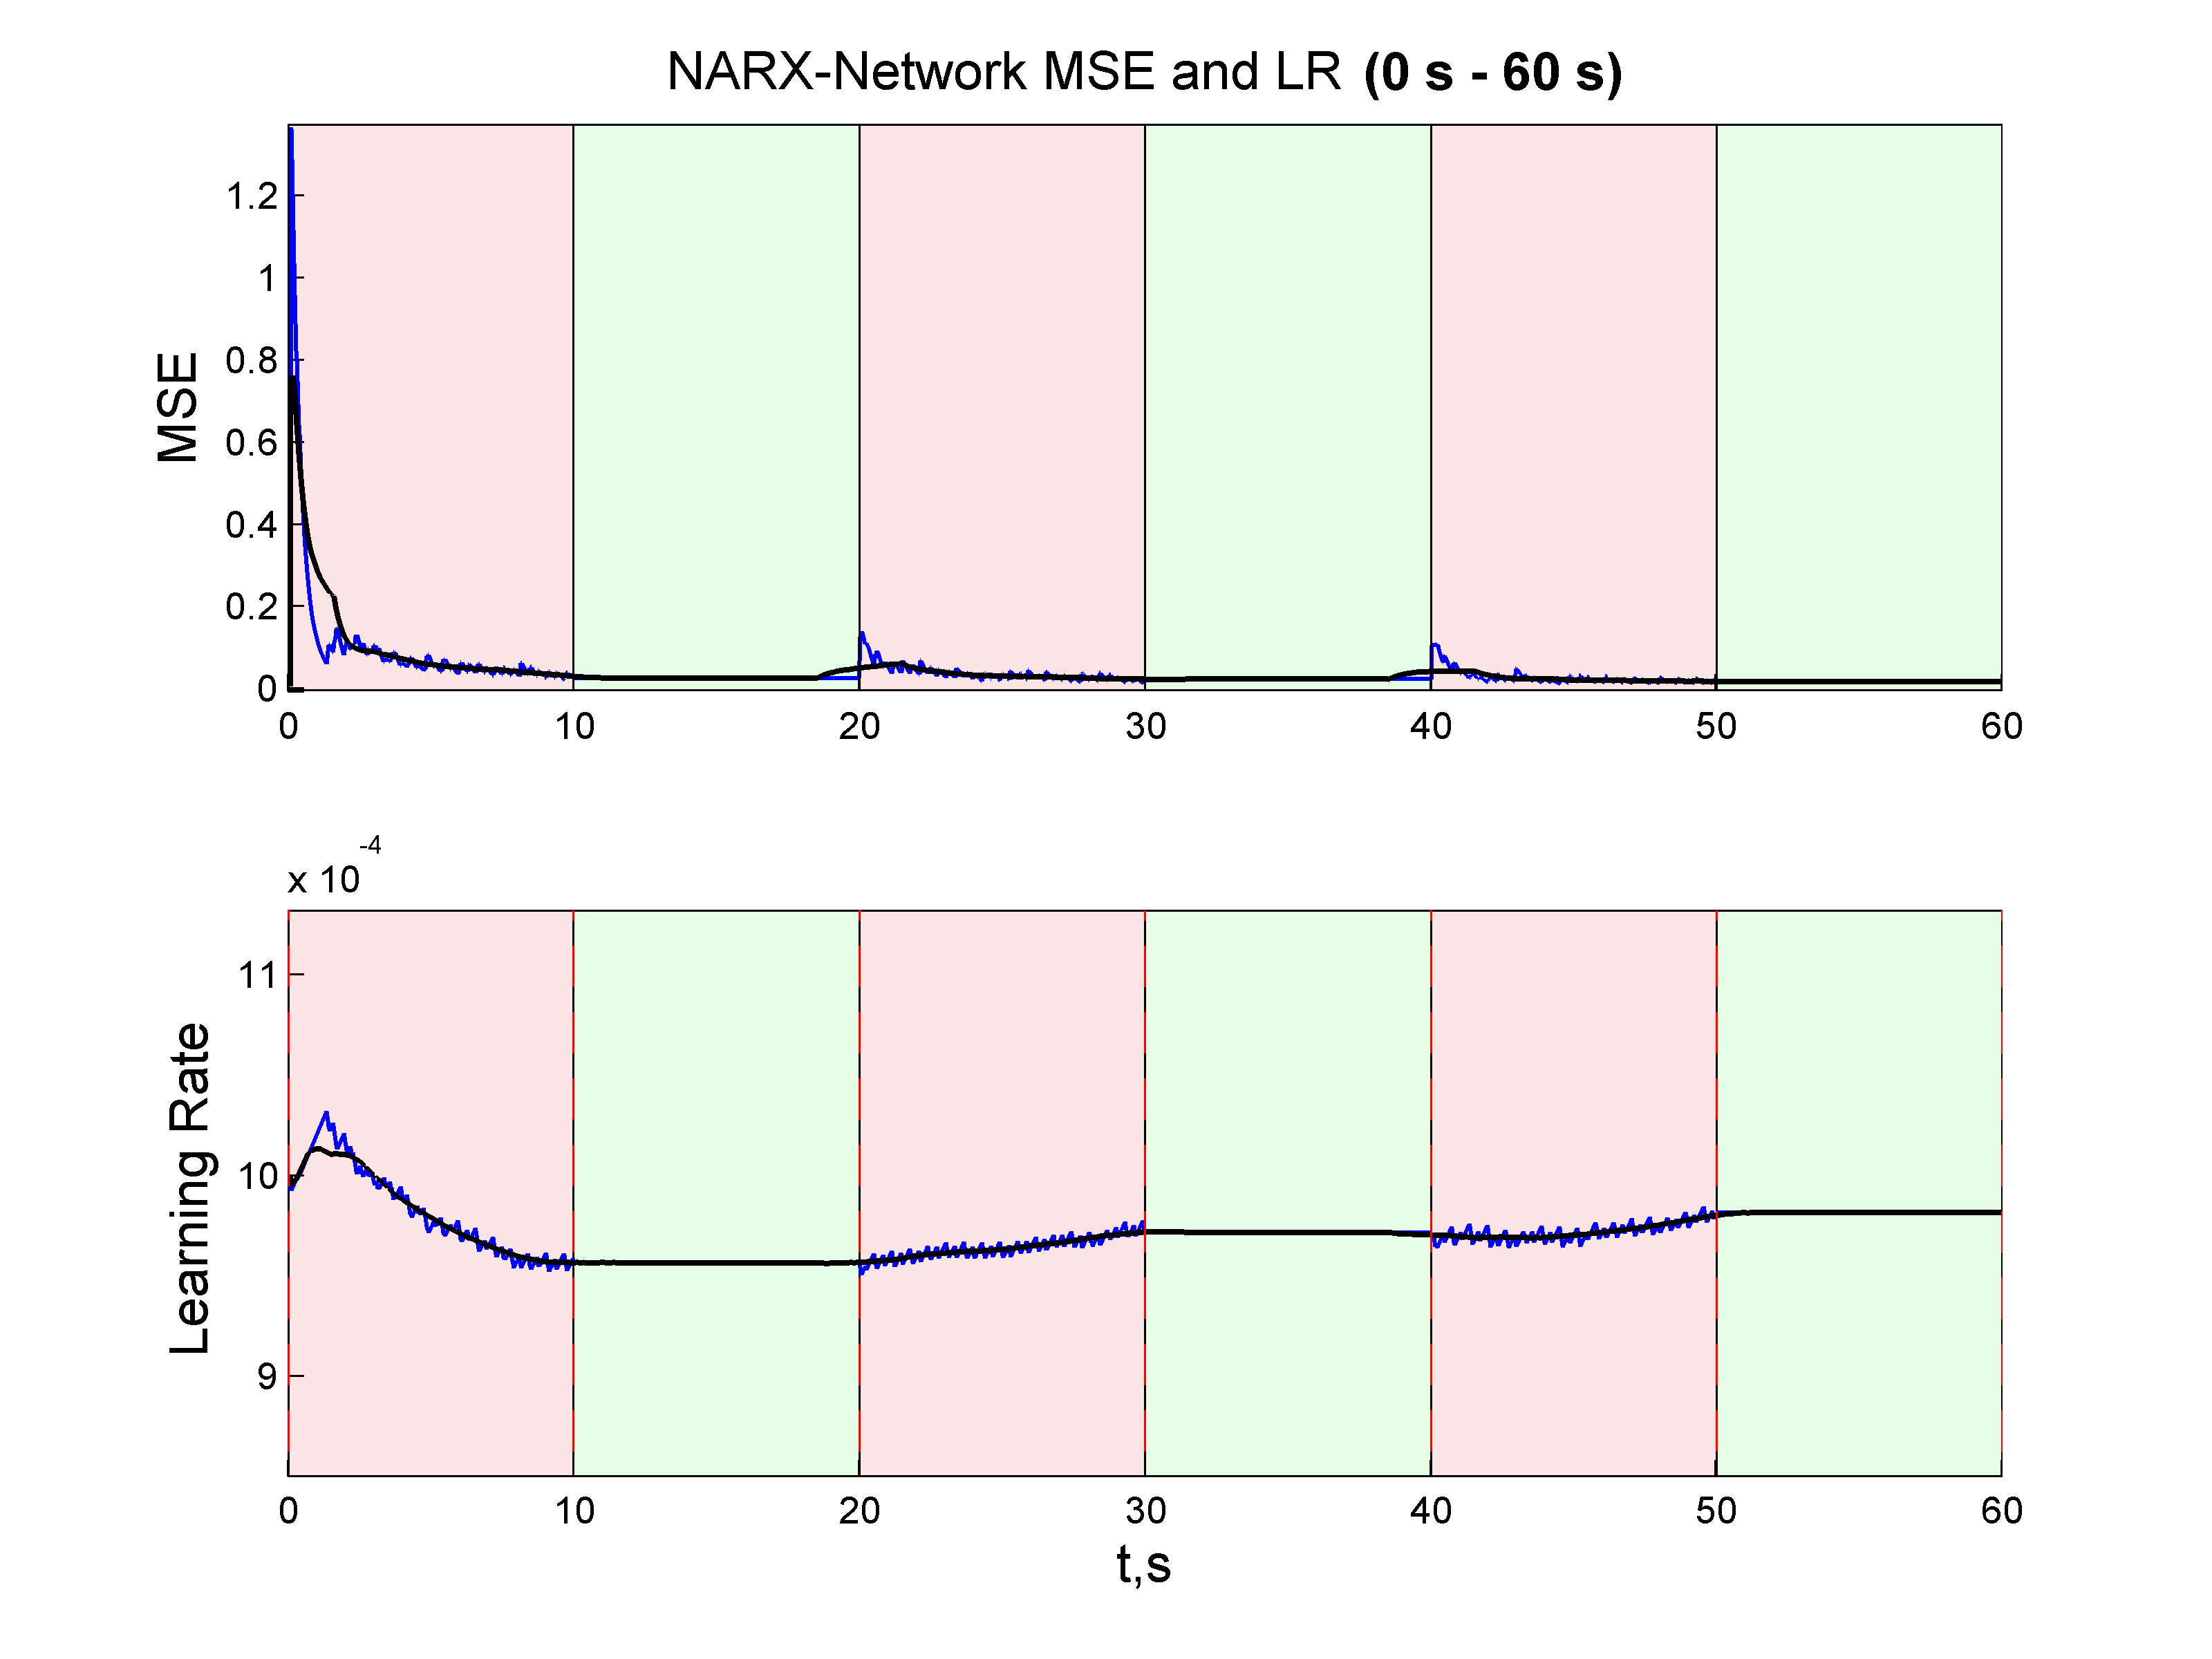
\includegraphics[width=0.85\textwidth]{aux_V_100mms_nN_50_nL_2_nns.png}}
					\caption{NARX Network MSE convergence for trial shown in Figure \ref{fig::narx100_a35}} 
					\label{fig::narx100_a35_nne}
				\end{figure}
				\begin{figure}
					\centering
					\fbox{ 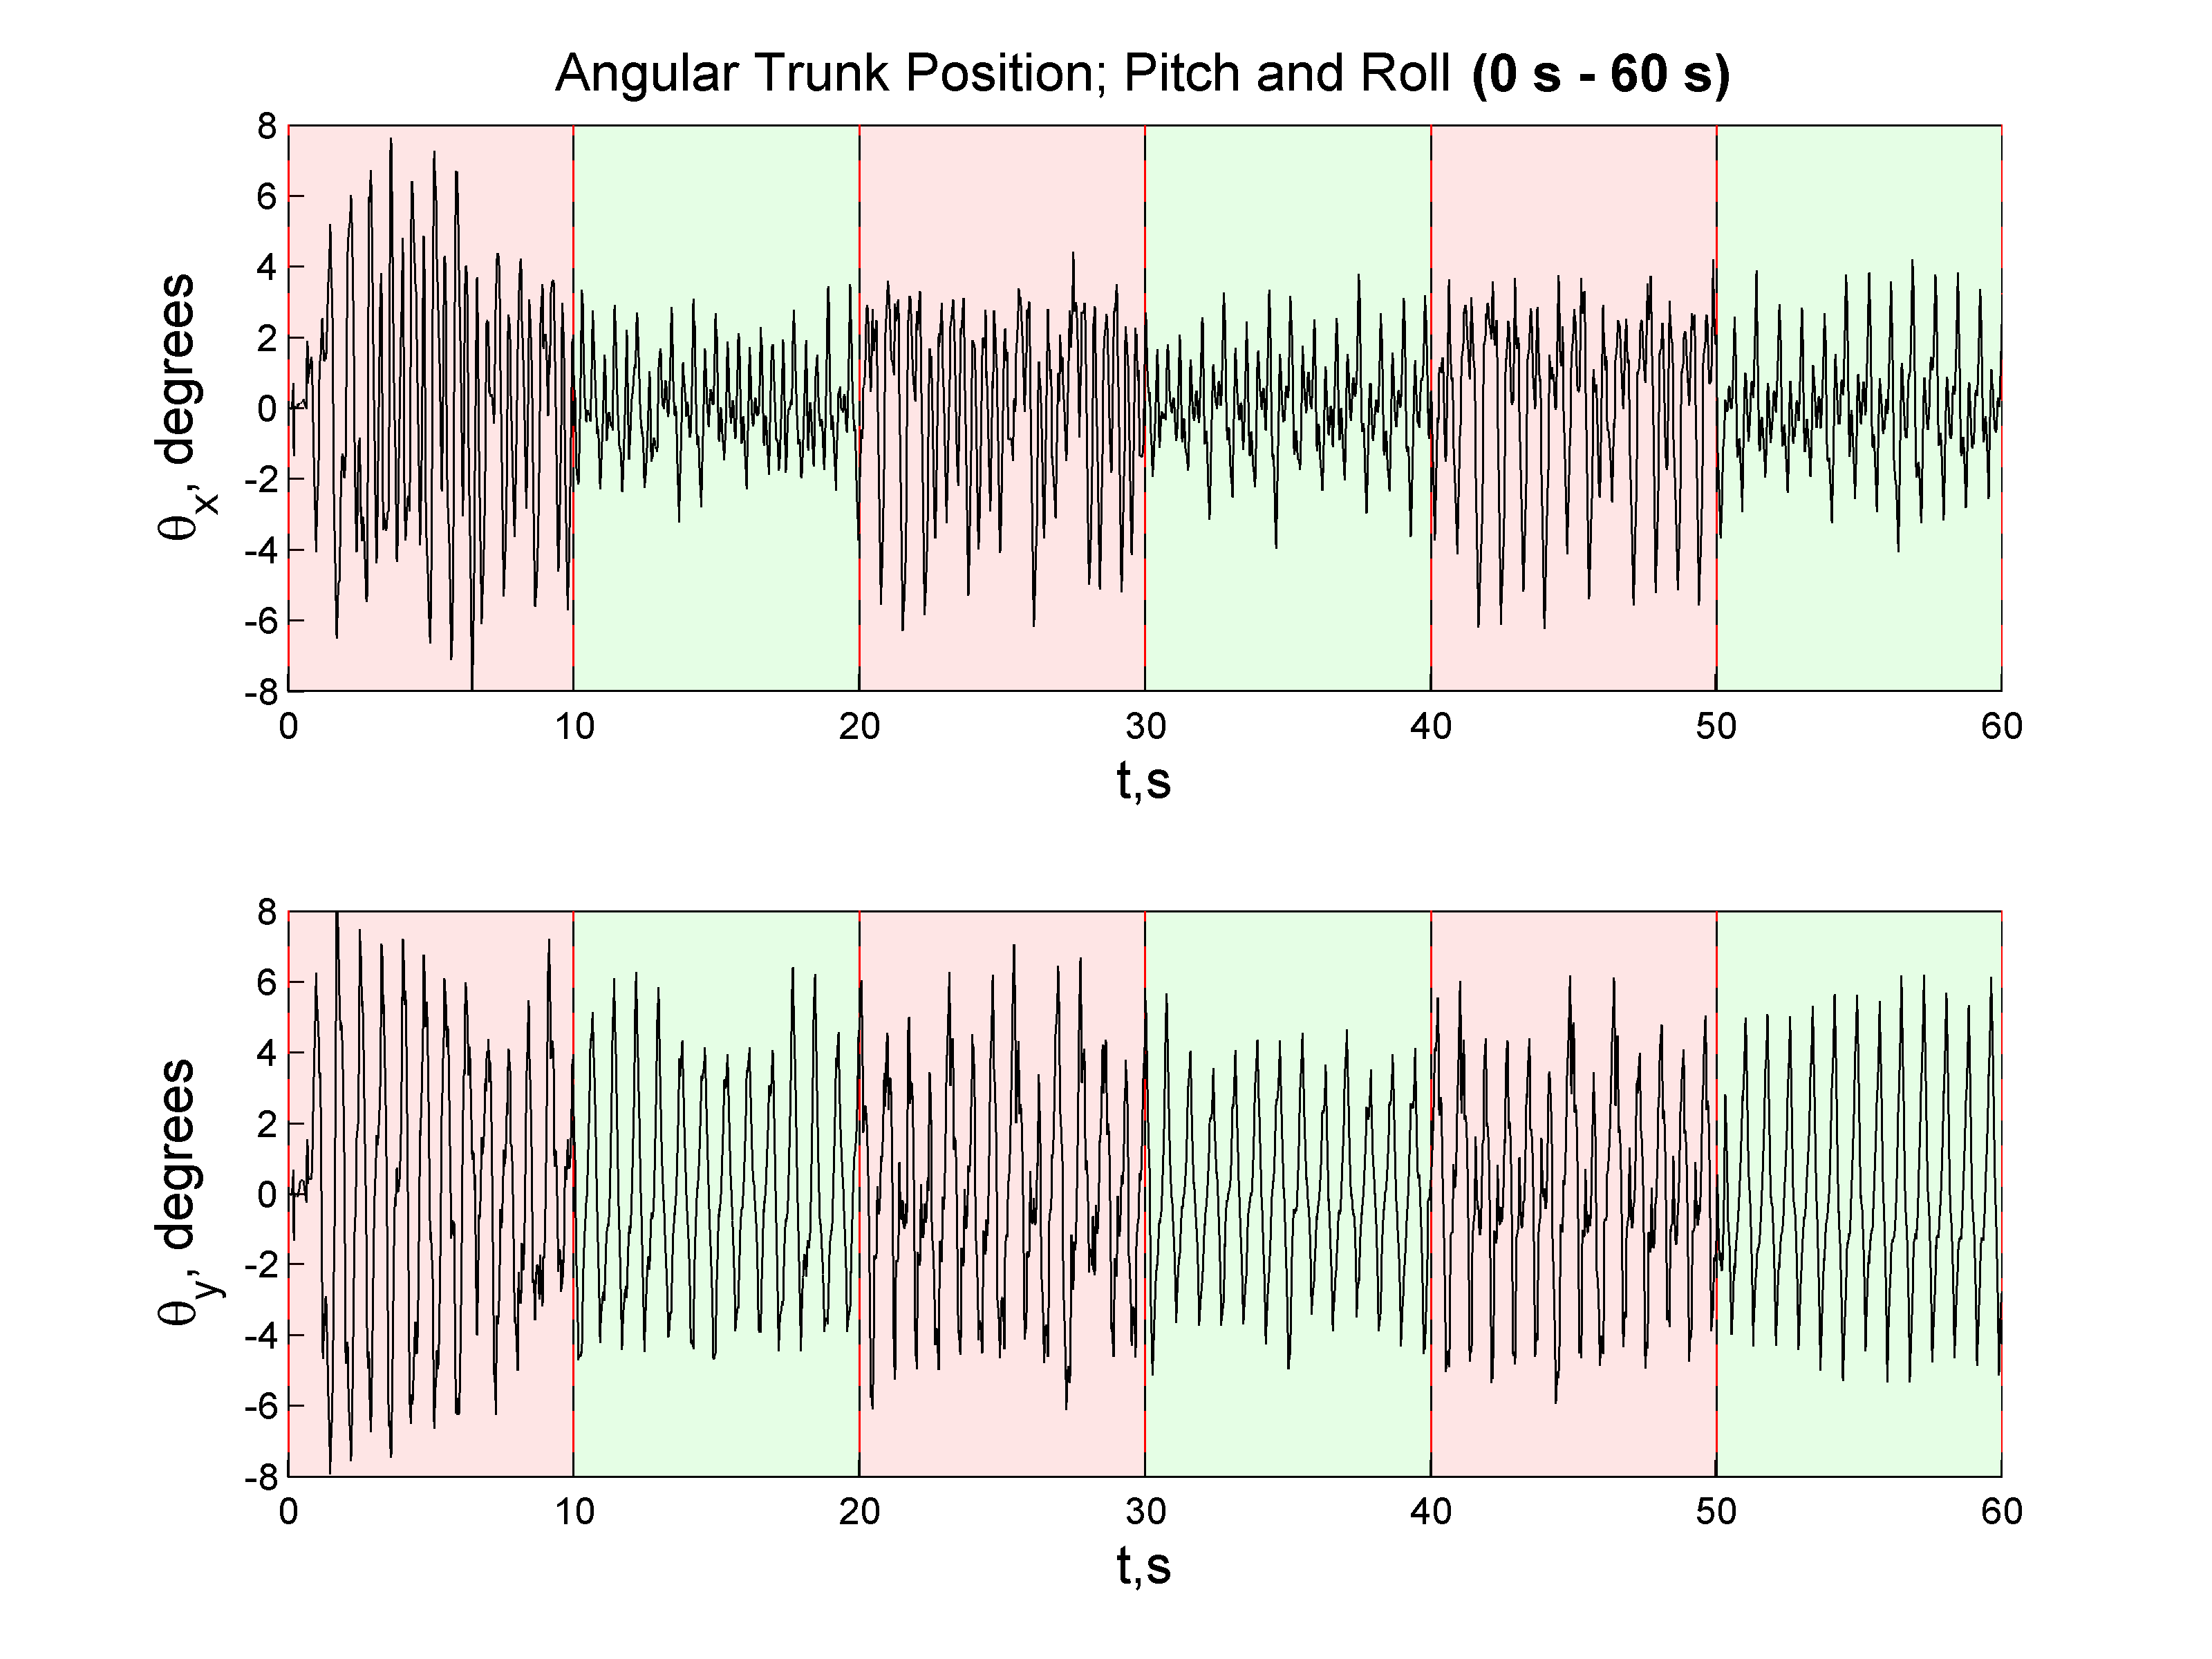
\includegraphics[width=0.85\textwidth]{alpha0125_V_60mms_nN_50_nL_2_pos.png} }
					\caption{Trunk orientation during 60 $\frac{mm}{s}$ gait with mixing parameter set to $\alpha = 0.125$.}
					\label{fig::narx60_a125_nne}
				\end{figure}
				\begin{figure}
					\centering
					\fbox{ 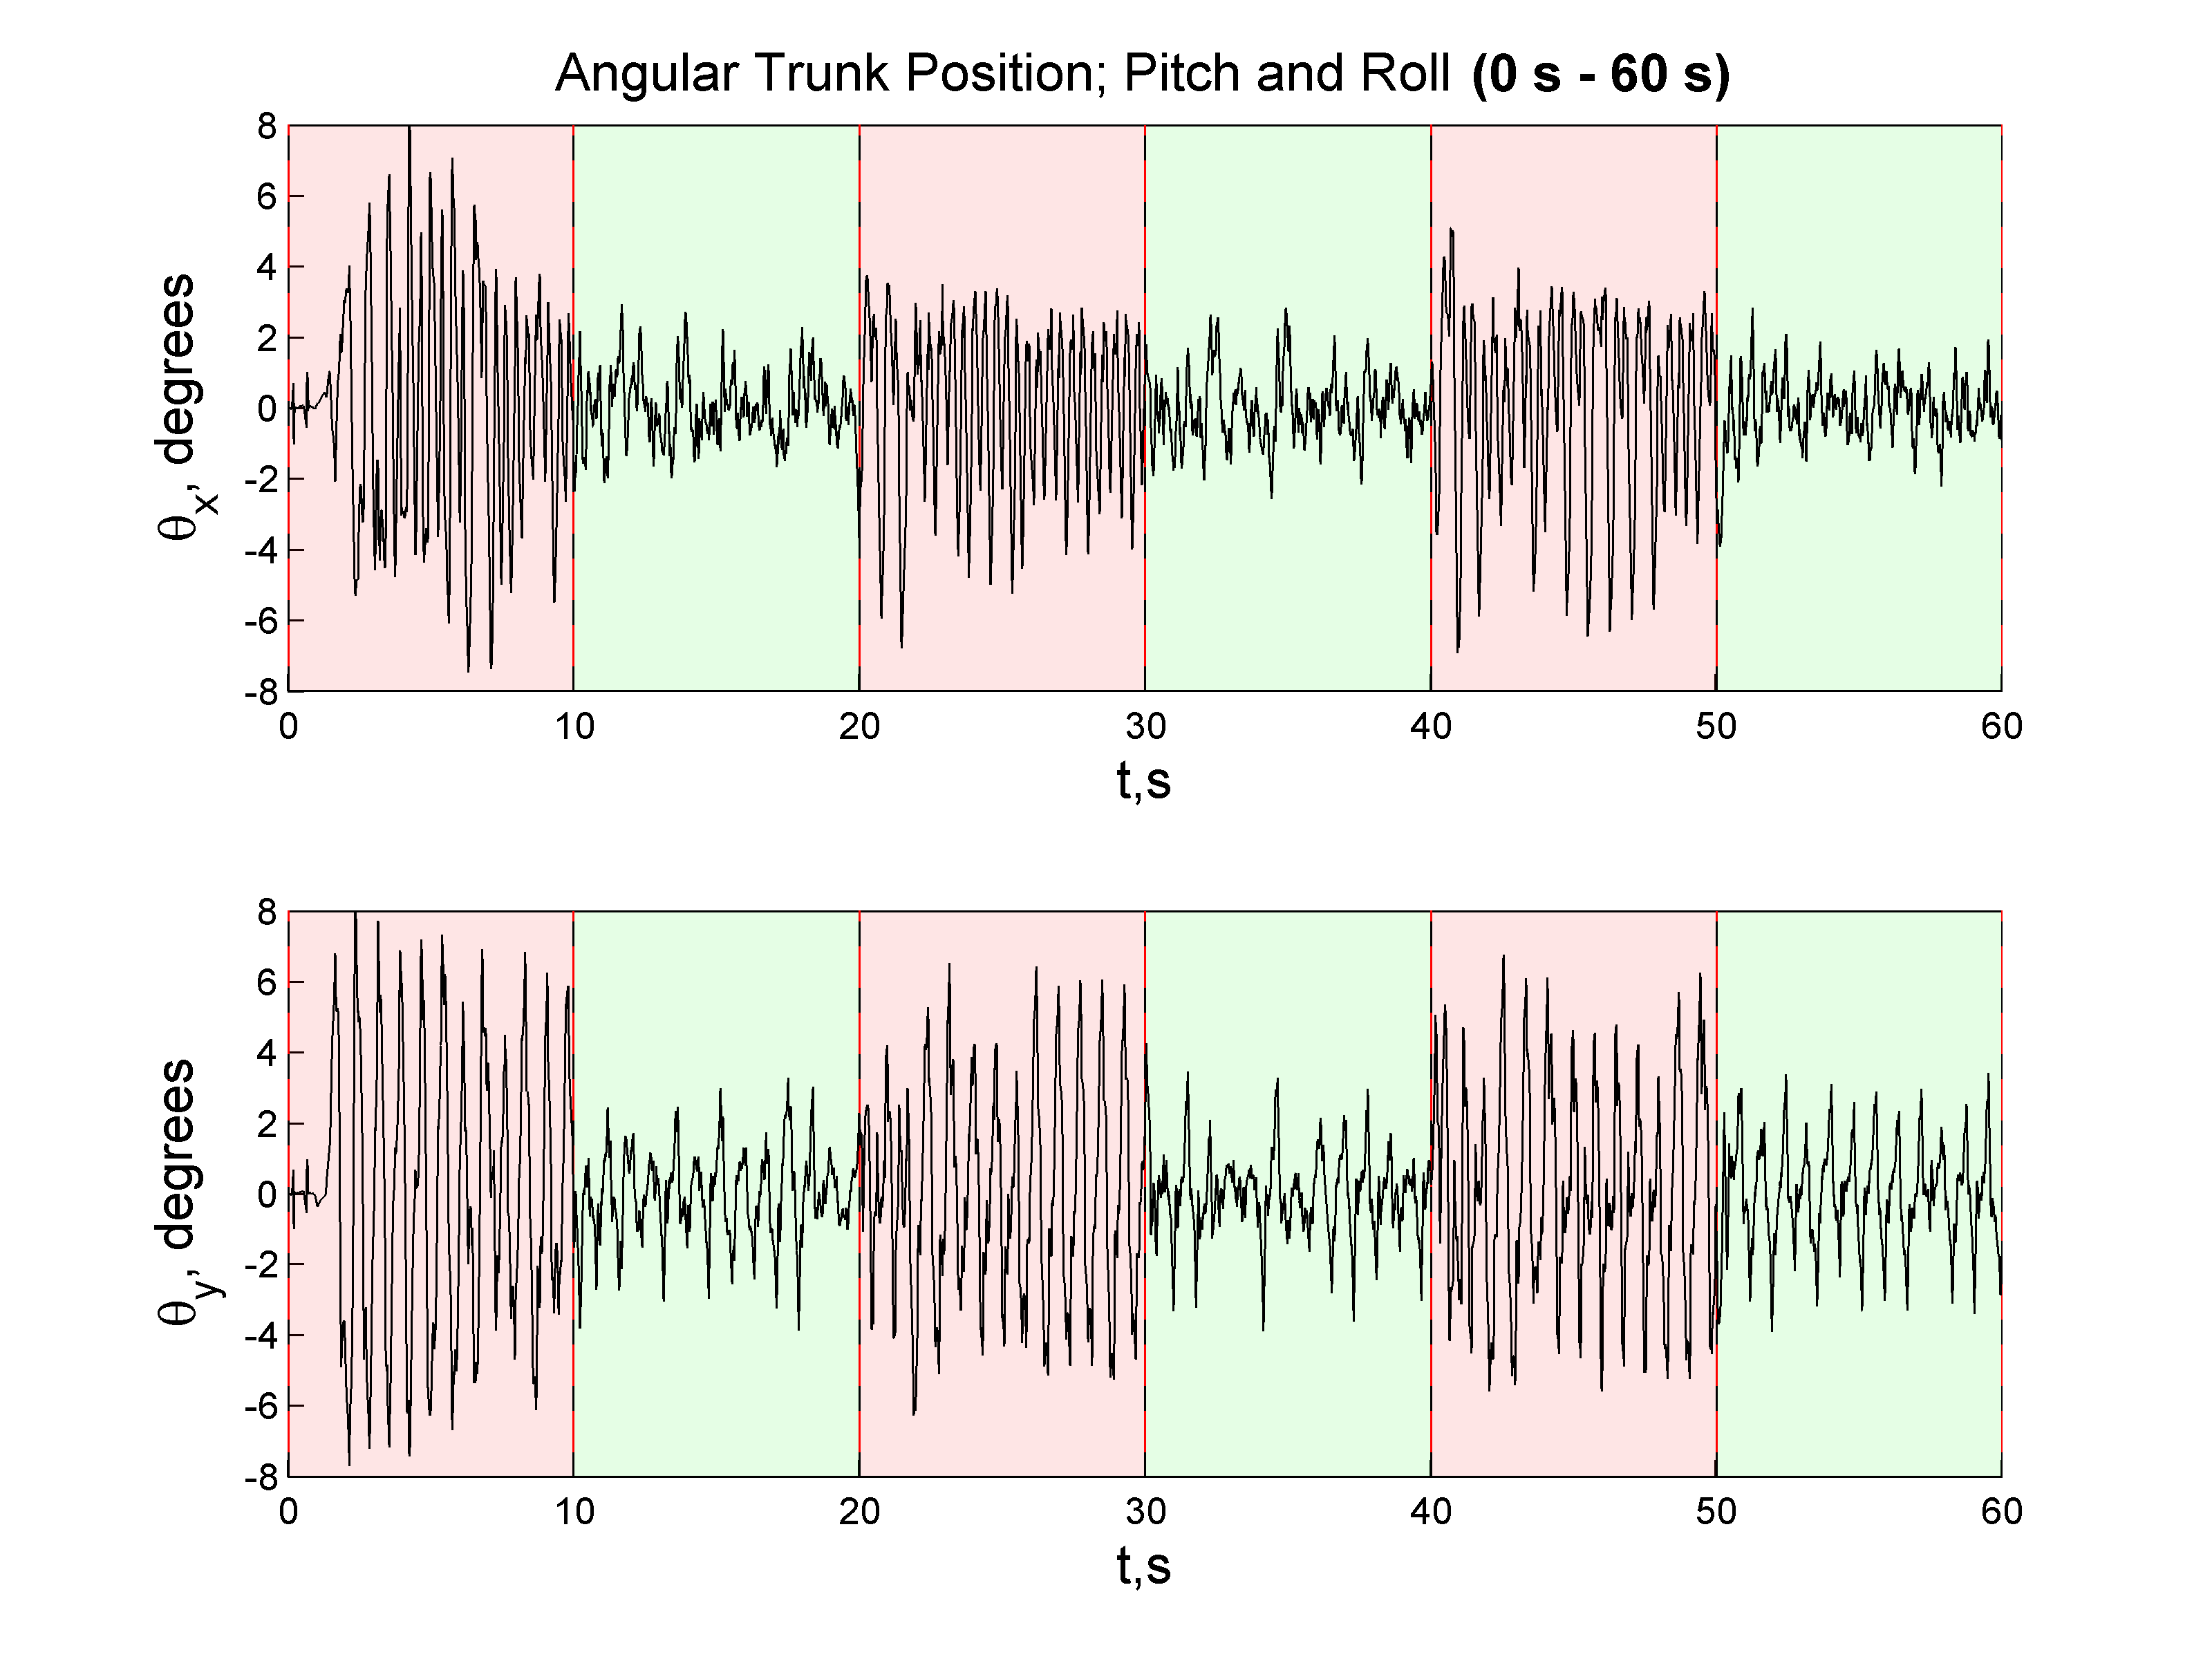
\includegraphics[width=0.85\textwidth]{alpha0250_V_60mms_nN_50_nL_2_pos.png} }
					\caption{Trunk orientation during 60 $\frac{mm}{s}$ gait with mixing parameter set to $\alpha = 0.250$.}
					\label{fig::narx60_a250_nne}
				\end{figure}
				\begin{figure}
					\centering
					\fbox{ 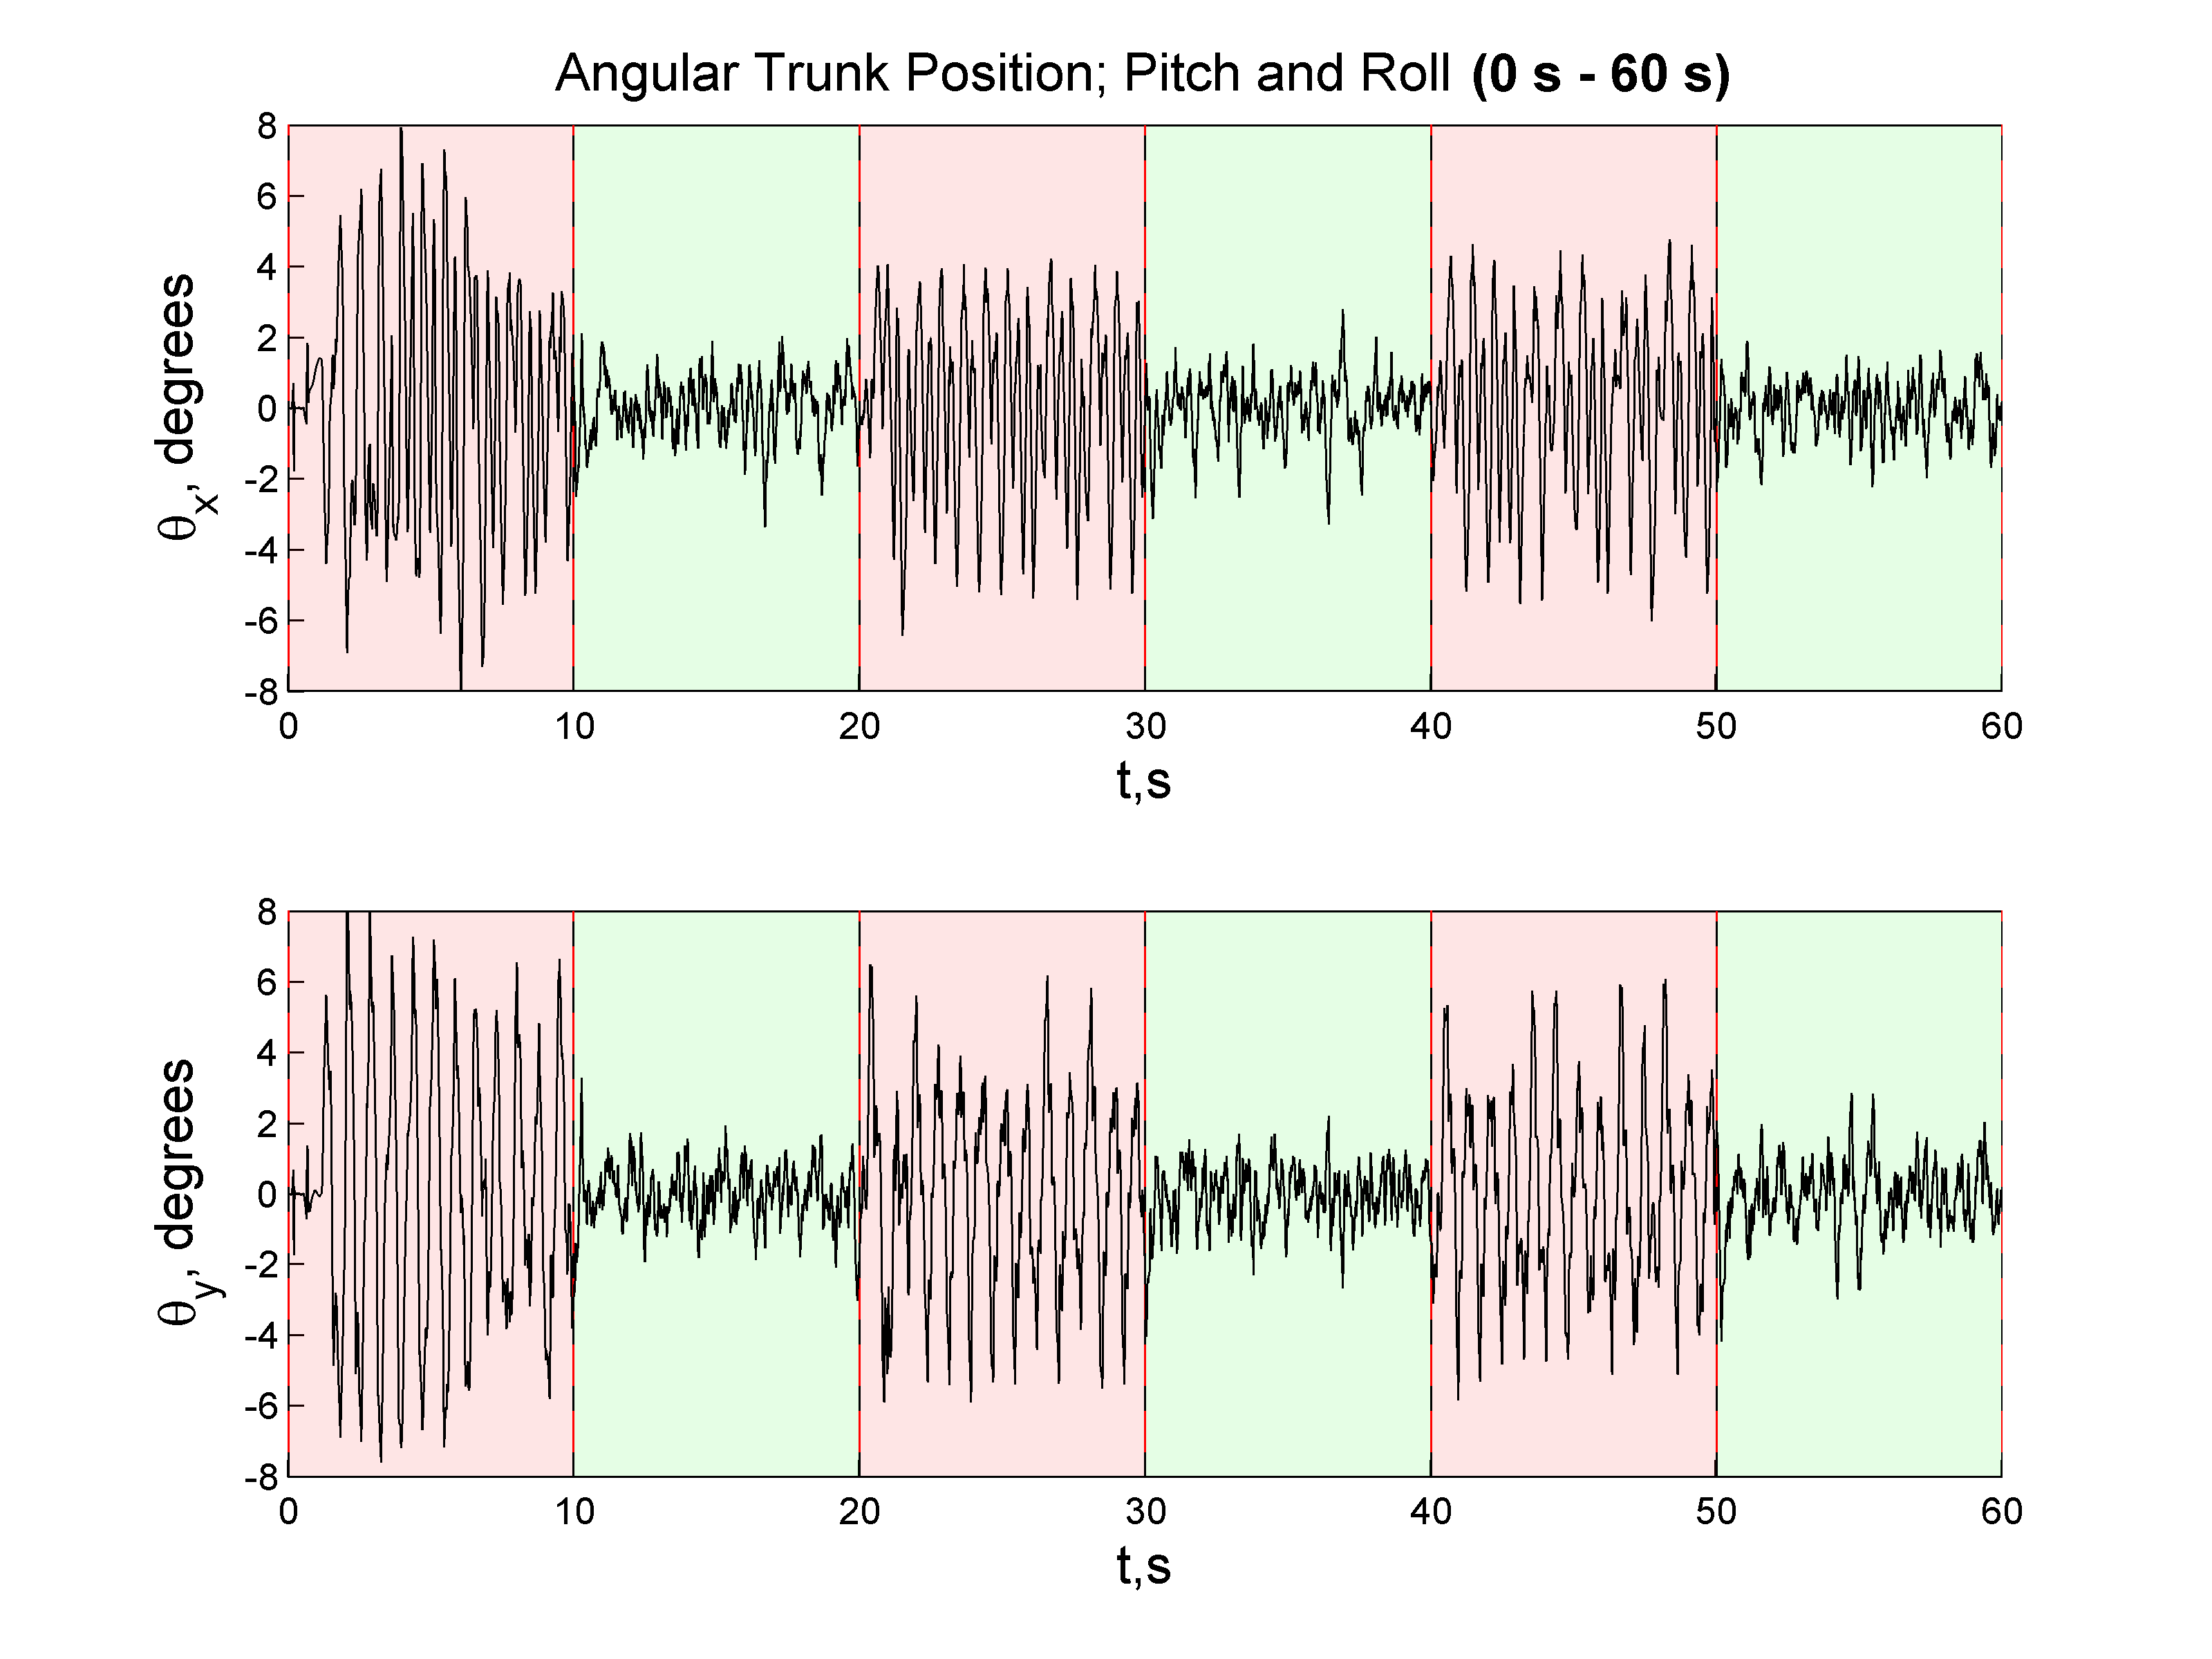
\includegraphics[width=0.85\textwidth]{alpha0350_V_60mms_nN_50_nL_2_pos.png} }
					\caption{Trunk orientation during 60 $\frac{mm}{s}$ gait with mixing parameter set to $\alpha = 0.350$.}
					\label{fig::narx60_a350_nne}
				\end{figure}
				\begin{figure}[!h]
					\centering
					\fbox{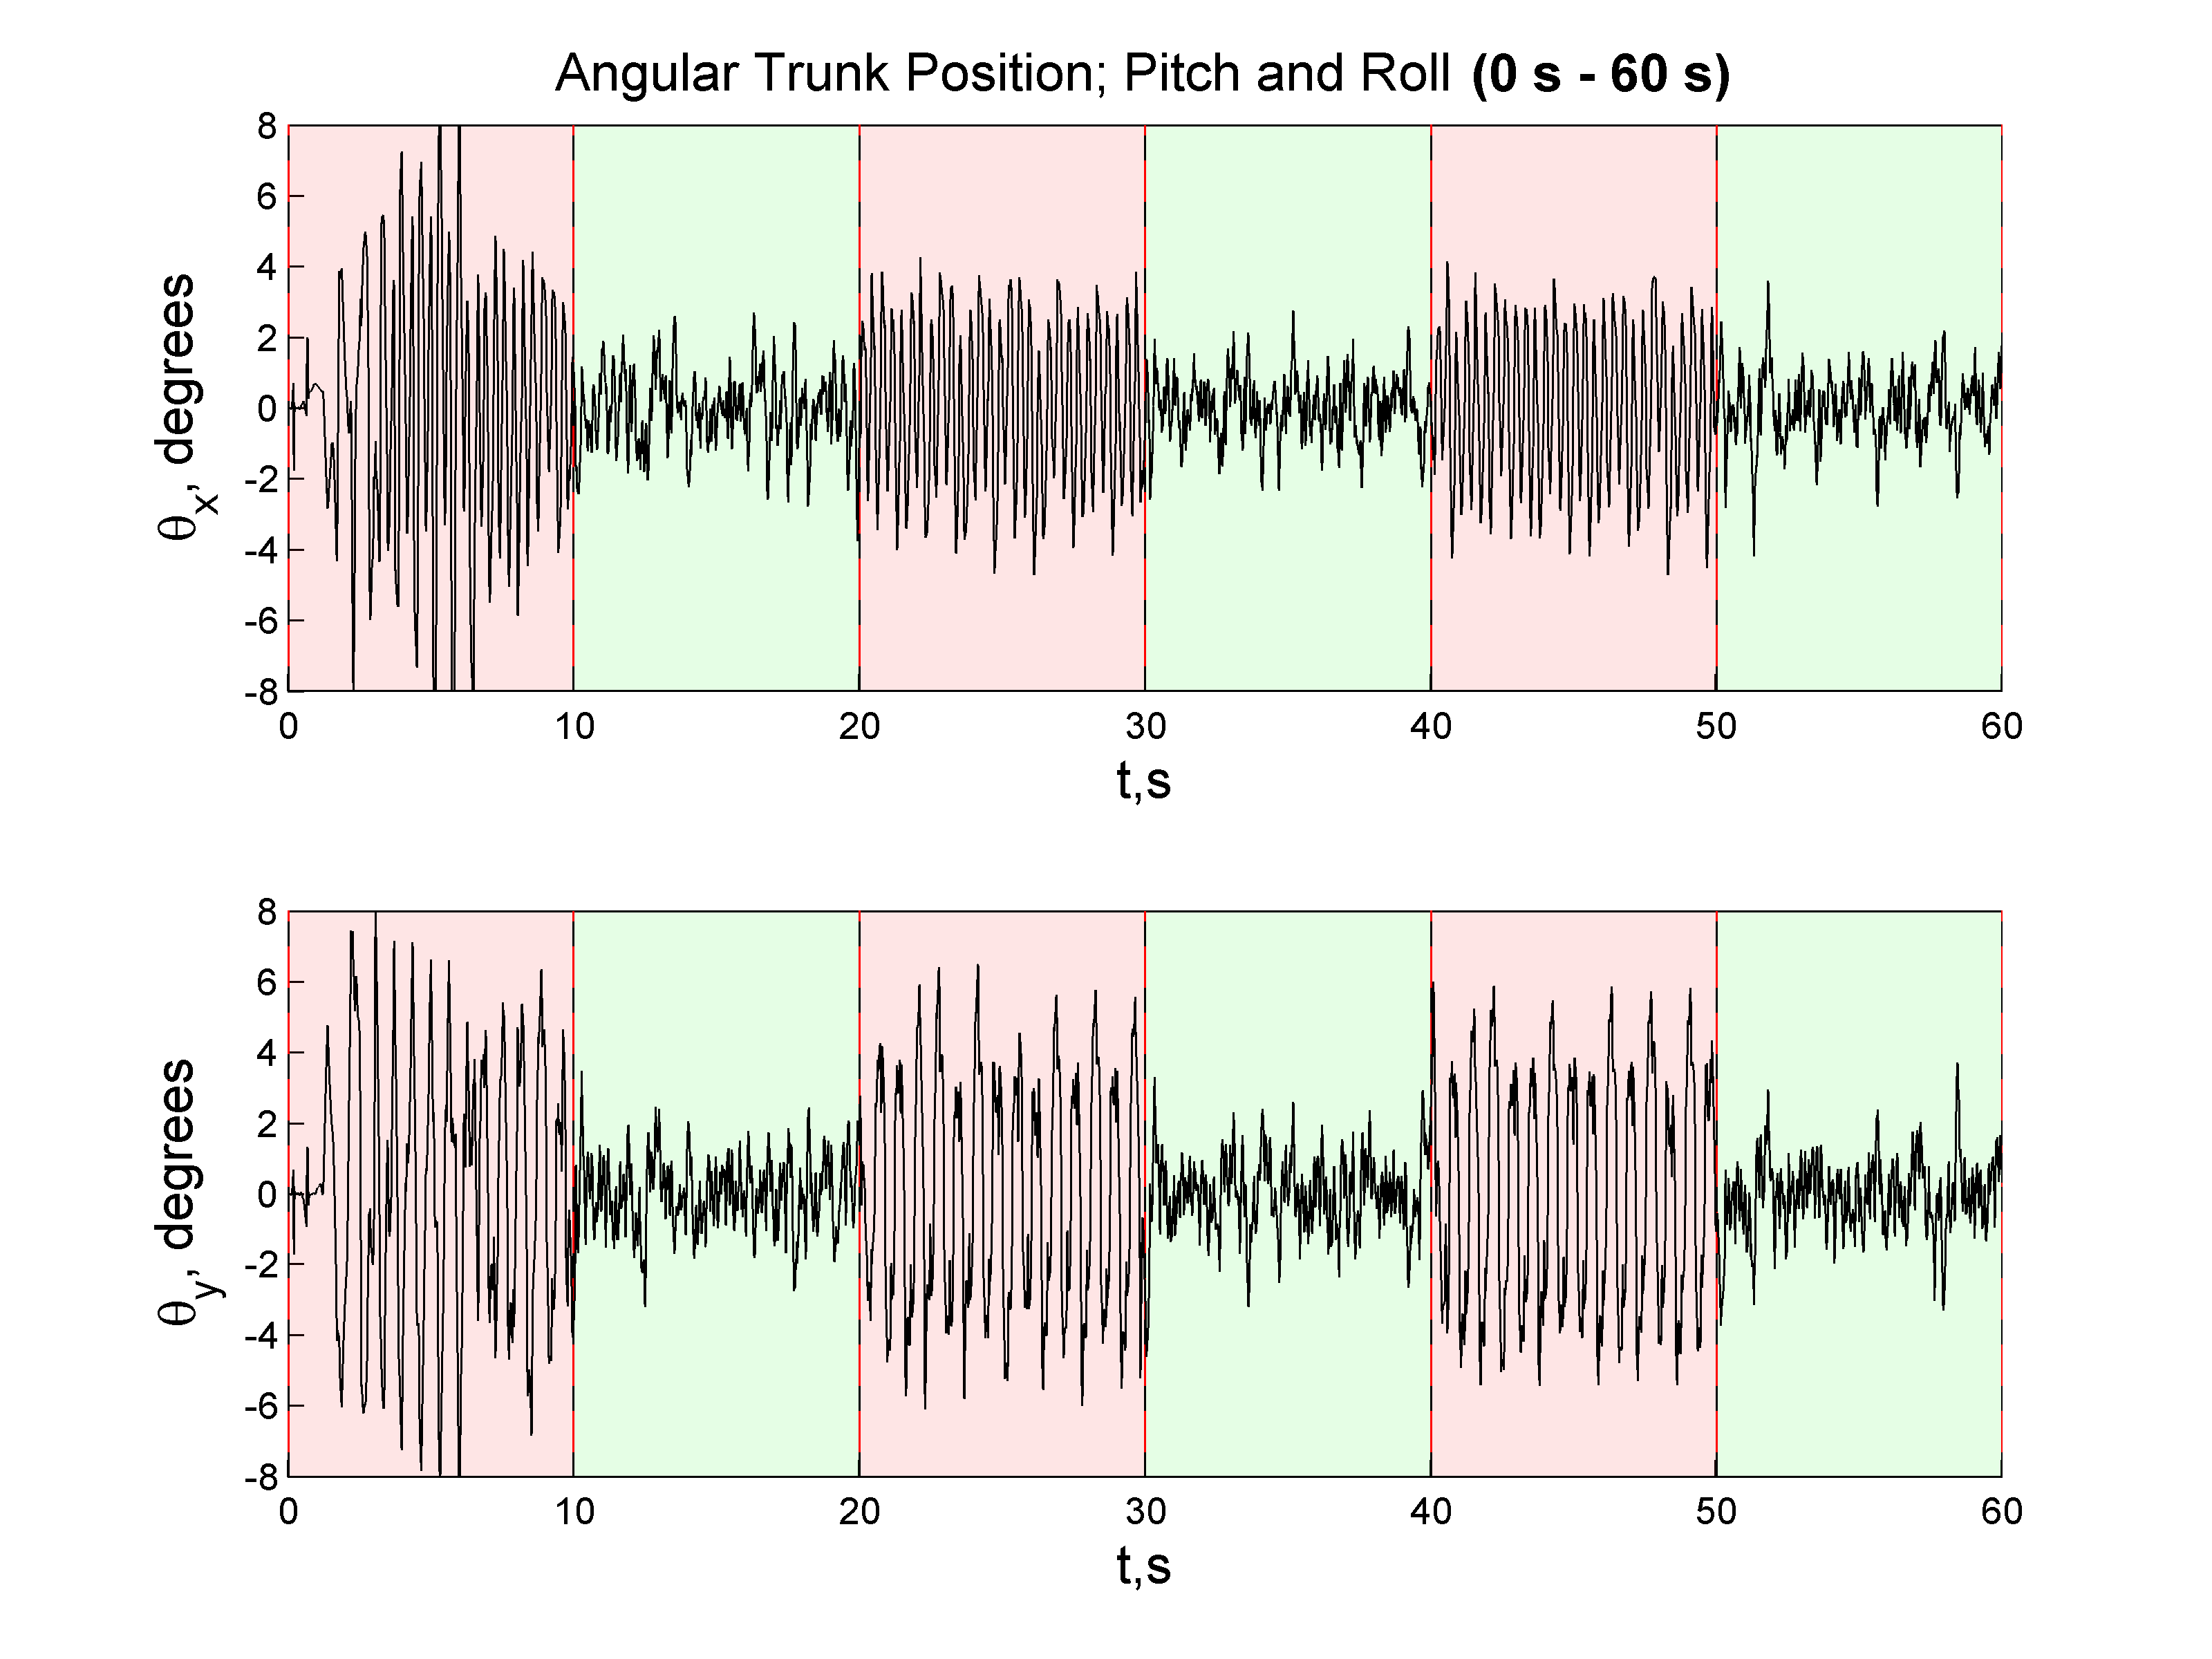
\includegraphics[width=0.85\textwidth]{aux_V_80mms_nN_50_nL_2_pos.png}}
					\caption{Trunk orientation during 80 $\frac{mm}{s}$ gait with mixing  parameter set to $\alpha = 0.35$}
					\label{fig::narx80_a35}
				\end{figure}
				\begin{figure}[!h]
					\centering
					\fbox{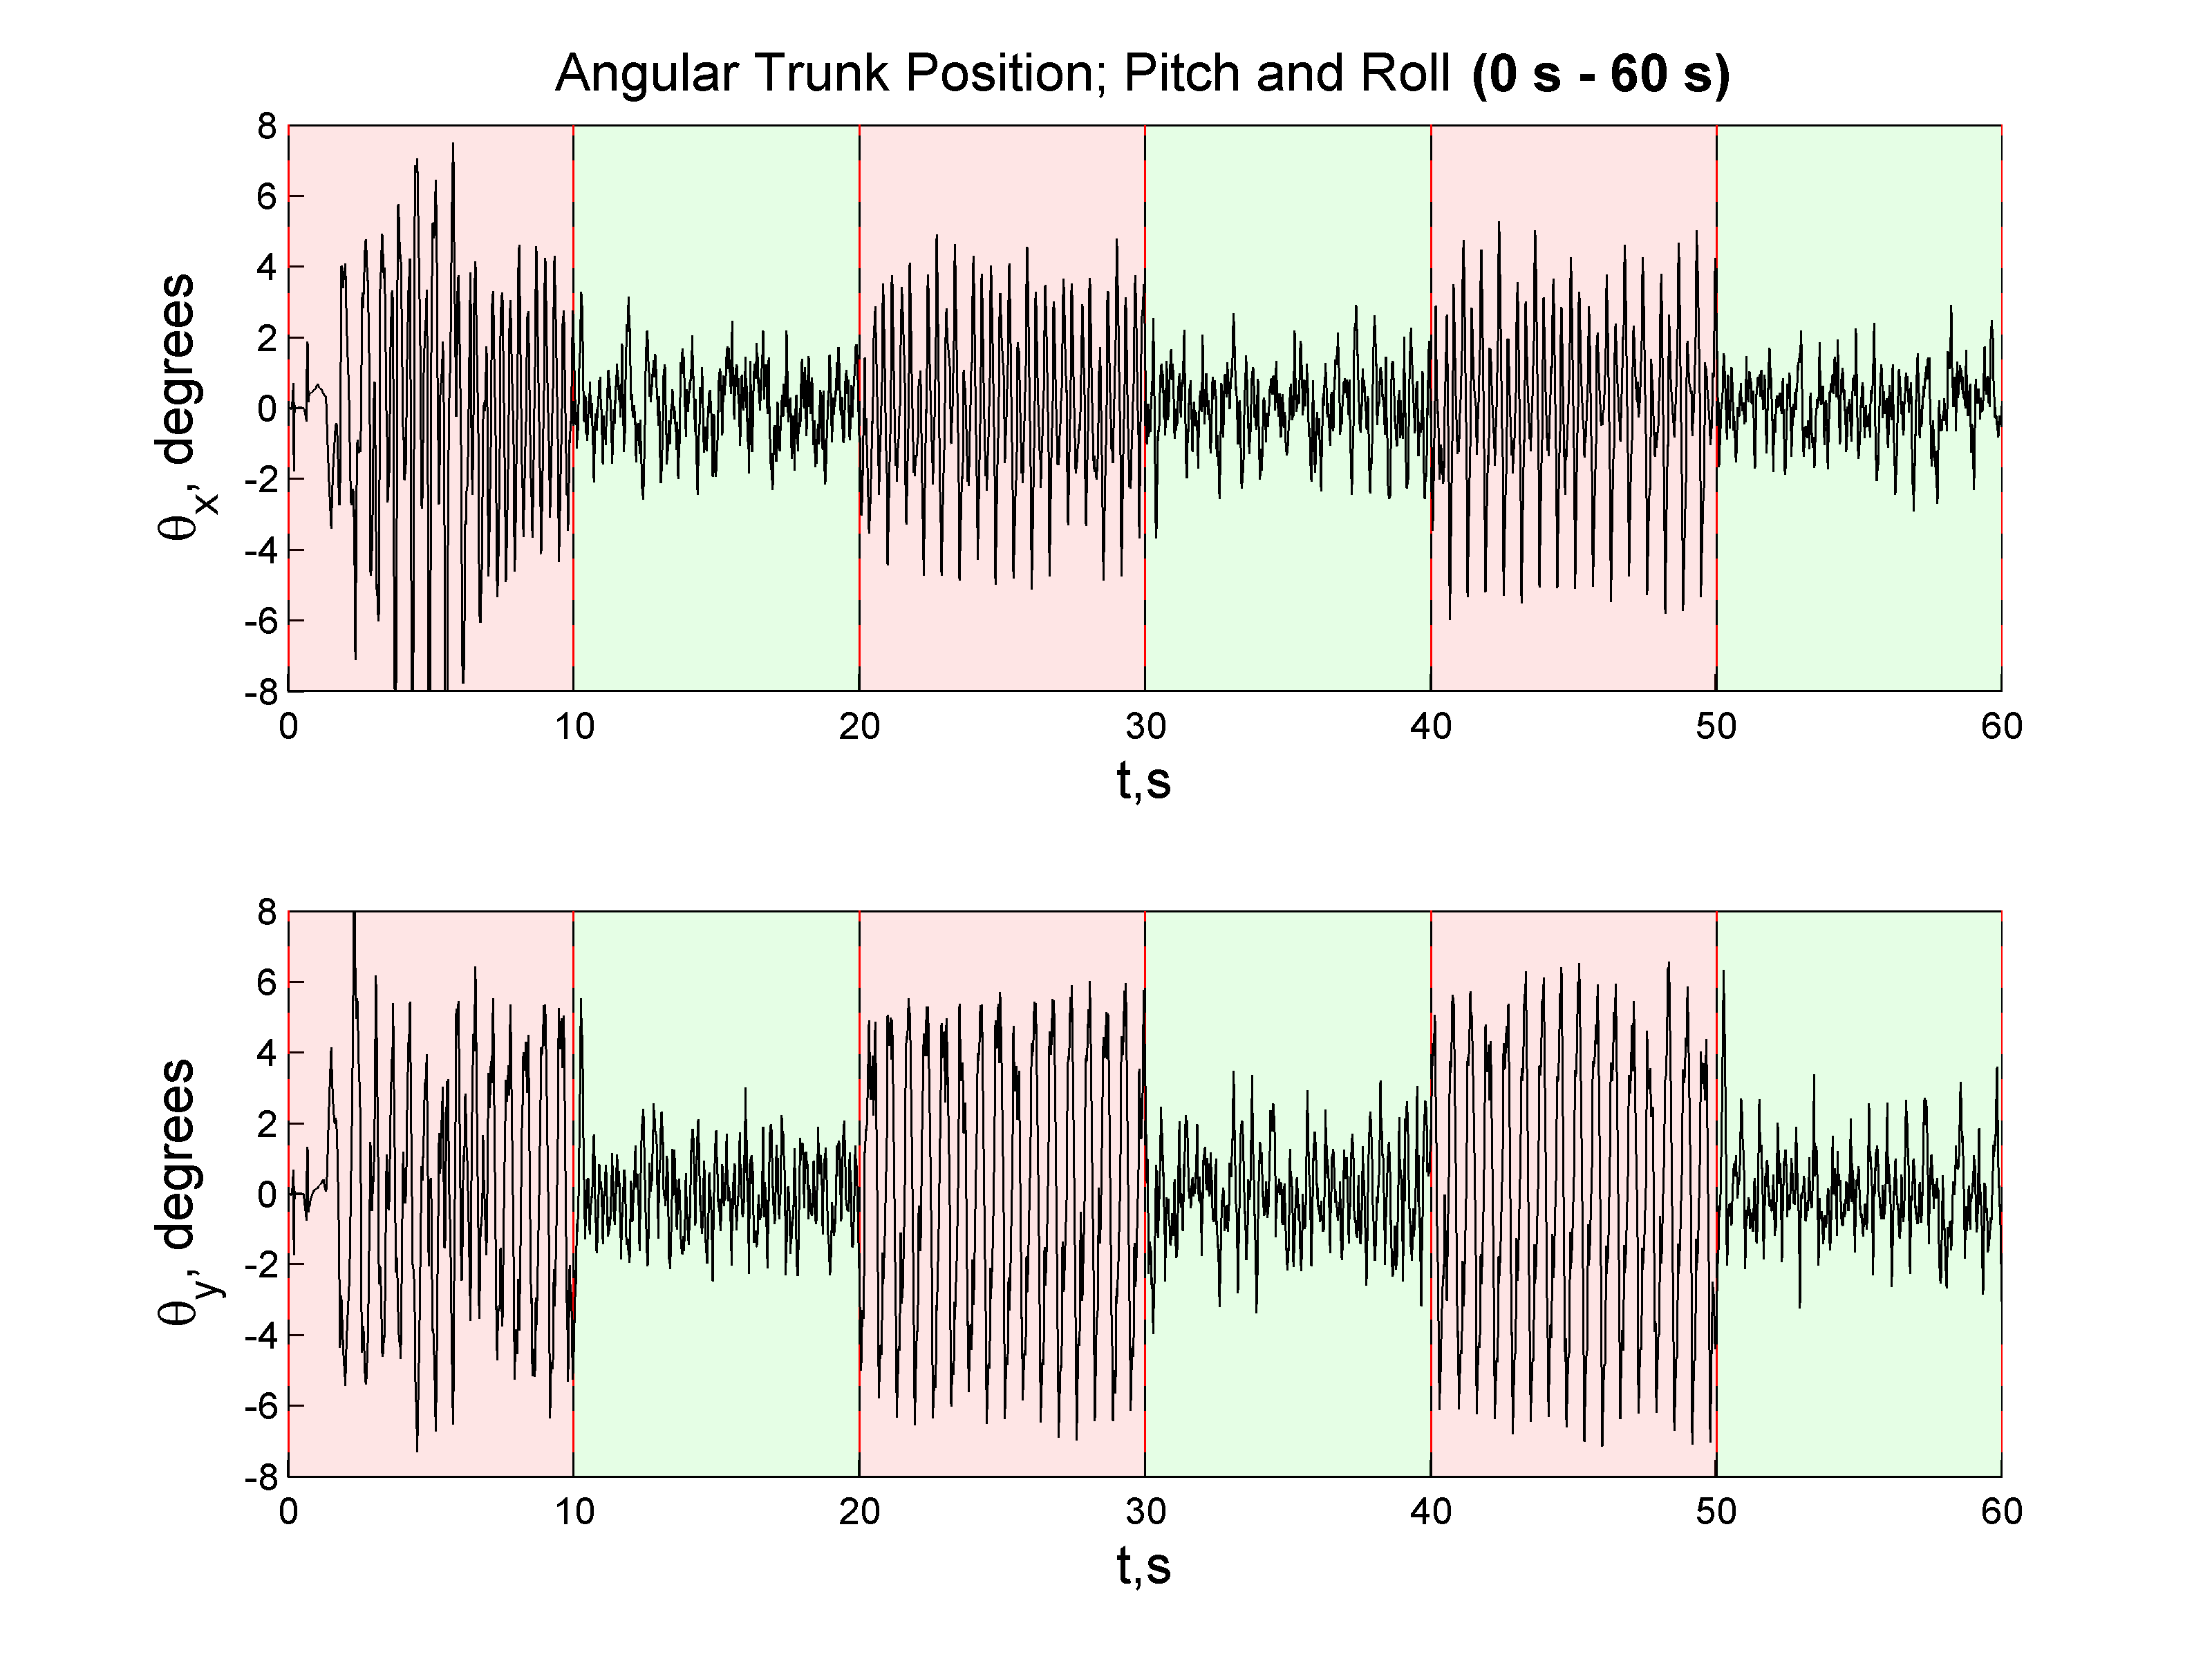
\includegraphics[width=0.85\textwidth]{aux_V_100mms_nN_50_nL_2_pos.png}}
					\caption{Trunk orientation during 100 $\frac{mm}{s}$ gait with mixing parameter set to $\alpha = 0.35$} 
					\label{fig::narx100_a35}
				\end{figure}
	%%%%%%%%%%%%%%%%%%%%%%%%%%%%%%%%%%%%%%%%%%%%%%%%%%%%%%%%%%%%%%%%%%%%%%%%%%%%%%%%%%
%%% Navigation Control
%%%
%%%
%%%%%%%%%%%%%%%%%%%%%%%%%%%%%%%%%%%%%%%%%%%%%%%%%%%%%%%%%%%%%%%%%%%%%%%%%%%%%%%%%%
\chapter{Perception and Navigation}
\label{ch::navigation}


	\section{Flatland navigation and Goal Tracking}
	
		The BlueFoot robot has been operated using potential field-based control-schemes for obstacle avoidance and camera-based goal-tracking over flatland. Platform navigation is administered by two main command parameters, $v^{r}$ and $\omega^{r}$, which represent forward and turning rate of the platform with respect to the robot's trunk frame $O_{b}$. During navigation, the pitch of the trunk, $\theta_{b,x}$ is also controlled via its respective reference signal, $\theta_{b,x}^{r}$. This control over trunk pose allows for additional articulation of the LIDAR and camera sensors mounted to BlueFoot's head. 

		BlueFoot's base navigation and obstacle avoidance algorithm involves a potential fields-based approach which fuses LIDAR data and features from processed camera images. This algorithm is essentially used as a ``wandering" mechanism which would normally be employed as a first-level navigation measure in an unknown environment when no information (\EG map data) is known by the robot \emph{apriori}. Camera features are used in conjunction with LIDAR scans for the purpose of assigning trackable targets, which can avoid local minima faced with navigating via a potential-fields approach. Notably, this navigation approach uses only 2D LIDAR data (does not take into account features of terrain) and is thus most fit for navigation over flatland.

		\subsection{LIDAR-based Potential-Fields Algorithm}
			The LIDAR-base portion of this algorithm takes sequential, planar LIDAR scans as an input and generates an output in the form of a vectored navigation command, $\vec{V}_{L}^{r}\in \Re^{3}$, relative to the world frame, $O_{0}$, as defined in Section~\ref{ch::system_modeling_pos_kin}. Each point from a LIDAR scan is mapped to a corresponding scalar \emph{potential} which is used to influence the direction of the newly generated command. Given a LIDAR scan $S$ with 2D scan points, $x_{i}^{L}\in\emph{S}^{L}$, relative to the LIDARs local coordinate frame $O_{L}$, an output command vector is generated using a potential function $\{ f(x) : \Re^{3}\rightarrow \Re^{1} \}$, and a biasing function, $\{ g(x,\psi) : \Re^{3}\rightarrow \Re^{1} \}$, as follows:
%
				\begin{eqnarray}
				x_{i}  &=& P_{ \vec{z} } \wrap{ H_{b}^{0} H_{L}^{b} \Gamma_{L} x_{i}^{L} } \nonumber\\
				\bar{x}_{b,i} &=&  x_{i}-p_{b} \nonumber \\
				\vec{V}_{c} &=& \alpha_{c} \wrap{\sum_{x_{i}\in \emph{S}} |f(\bar{x}_{b,i})|_{1}}^{-1}  \wrap{ \sum_{x_{i} \in \emph{S}} g( \bar{x}_{b,i},\psi)  f( \bar{x}_{b,i} ) \frac{\bar{x}_{b,i}}{\norm{\bar{x}_{b,i}}} }
				\end{eqnarray}
			where $H_{b}^{0}$ defines a homogeneous transformation between $O_{0}$ and $O_{b}$; $H_{L}^{b}$ defines a homogeneous transformation which relates the LIDAR sensors pose to the frame $O_{b}$; $\emph{S}\subset \Re^{3}$ is the set of newly transformed points, $x_{i} \in \emph{S}$ which respect the current LIDAR scan in the world coordinate system; $\alpha_{c}$ is a scalar tuning parameter; and 
				\begin{equation*}
					\Gamma_{L} = \sbrack{ I_{2\times2}, 0_{2\times1} }^{T}.
				\end{equation*}
			Since we are assuming navigation over flat ground, the operator $P_{ \vec{z} }\wrap{*}$ is used to project each transformed LIDAR scan-point onto the plane defined by the $z$-axis unit vector in the frame $O_{0}$.

			The piecewise-continuous potential function, defined in \ref{eq::min_dis_potential_function}, is used in BlueFoot's navigation scheme is designed to ``repel" the platform from objects which are at some minimum distance, $d_{min}$ from the trunk, and attracted toward objects that are further away. The form of this potential function is inspired by several potential function candidates for attractive/repulsive force-field functions presented in \cite{ArambulaCosio2004}. The function \ref{eq::min_dis_potential_function} tends to draw the robot towards long apertures, such as corridors or openings, and away from close-by obstructions. It is written as follows:
				\begin{eqnarray}
					\Delta d &\equiv& \norm{x}-d_{min} \nonumber \\
					f(x) &=& 
					\begin{cases}	
					 	\wrap{\Delta d} \lambda_{c,1}	&  \text{if } \Delta d < 0 \\
										\wrap{\Delta d} \wrap{ 1  - e^{ -  \lambda_{c,2} { \wrap{\Delta d} }^{2} } } 	&  \text{else}
					\end{cases}
				\label{eq::min_dis_potential_function}
				\end{eqnarray}
			where $\lambda_{c,1}>0$ and $\lambda_{c,2}>0$ are tuning parameters sued to specify the output range and sensitivity of the potential function output with respect to $\Delta d$, respectively. It can be observed that this potential function exhibits $f(x)<0$ when $\norm{x} < d_{min}$ and vice-verse, thus achieves the desired attractive/repulsive characteristics. Namely, this potential function favors points which are generally much further away from the robot, and applies \emph{strong} repulsive forces only when obstacles come within a close range with the platform. These characteristics offer a higher propensity for exploration when the area being navigated is very spacious with few obstacles in view (but at mid range), while encourgaing \emph{tight} navigation around potential obstacles. This typically advantageous when obstacles are close together, such as a floating object near a wall, as the robot is less likely to move torward another obstacle in the process of avering another.  

			The biasing function $g(x,\psi)$ is used to weight the effect of individual scan-point potentials, $f(x_{i}-p_{b})$, on the final navigation output, with respect to the angular-window parameter $\psi>0$. A simple masking-type biasing function is used in BlueFoot's navigation function, which is formally defined as follows:
				\begin{equation}
					g(x,\psi) = 
					\begin{cases}
					1	& \tan^{-1}\wrap{ \frac{x_{2}}{x_{1}} } < \psi \\
					0 	& \text{otherwise}.
					\end{cases}
				\end{equation}
			where $x_{1}$ and $x_{2}$ are the first and second elements of the vector argument $x\in\Re^{3}$. This function is used to give priority to ``foward" points within an angular window $\psi$ and serves to reduce the potential for getting stuck in local minima. A visualization of  the composite potential field, $f(x)g(x,\psi)$, with $\psi=\pi/2$ is shown in Figure \ref{fig::potential_field} for a $2$-by-$2$ meter area about the robot.
							\begin{figure}[t!]
								\centering
								\fbox{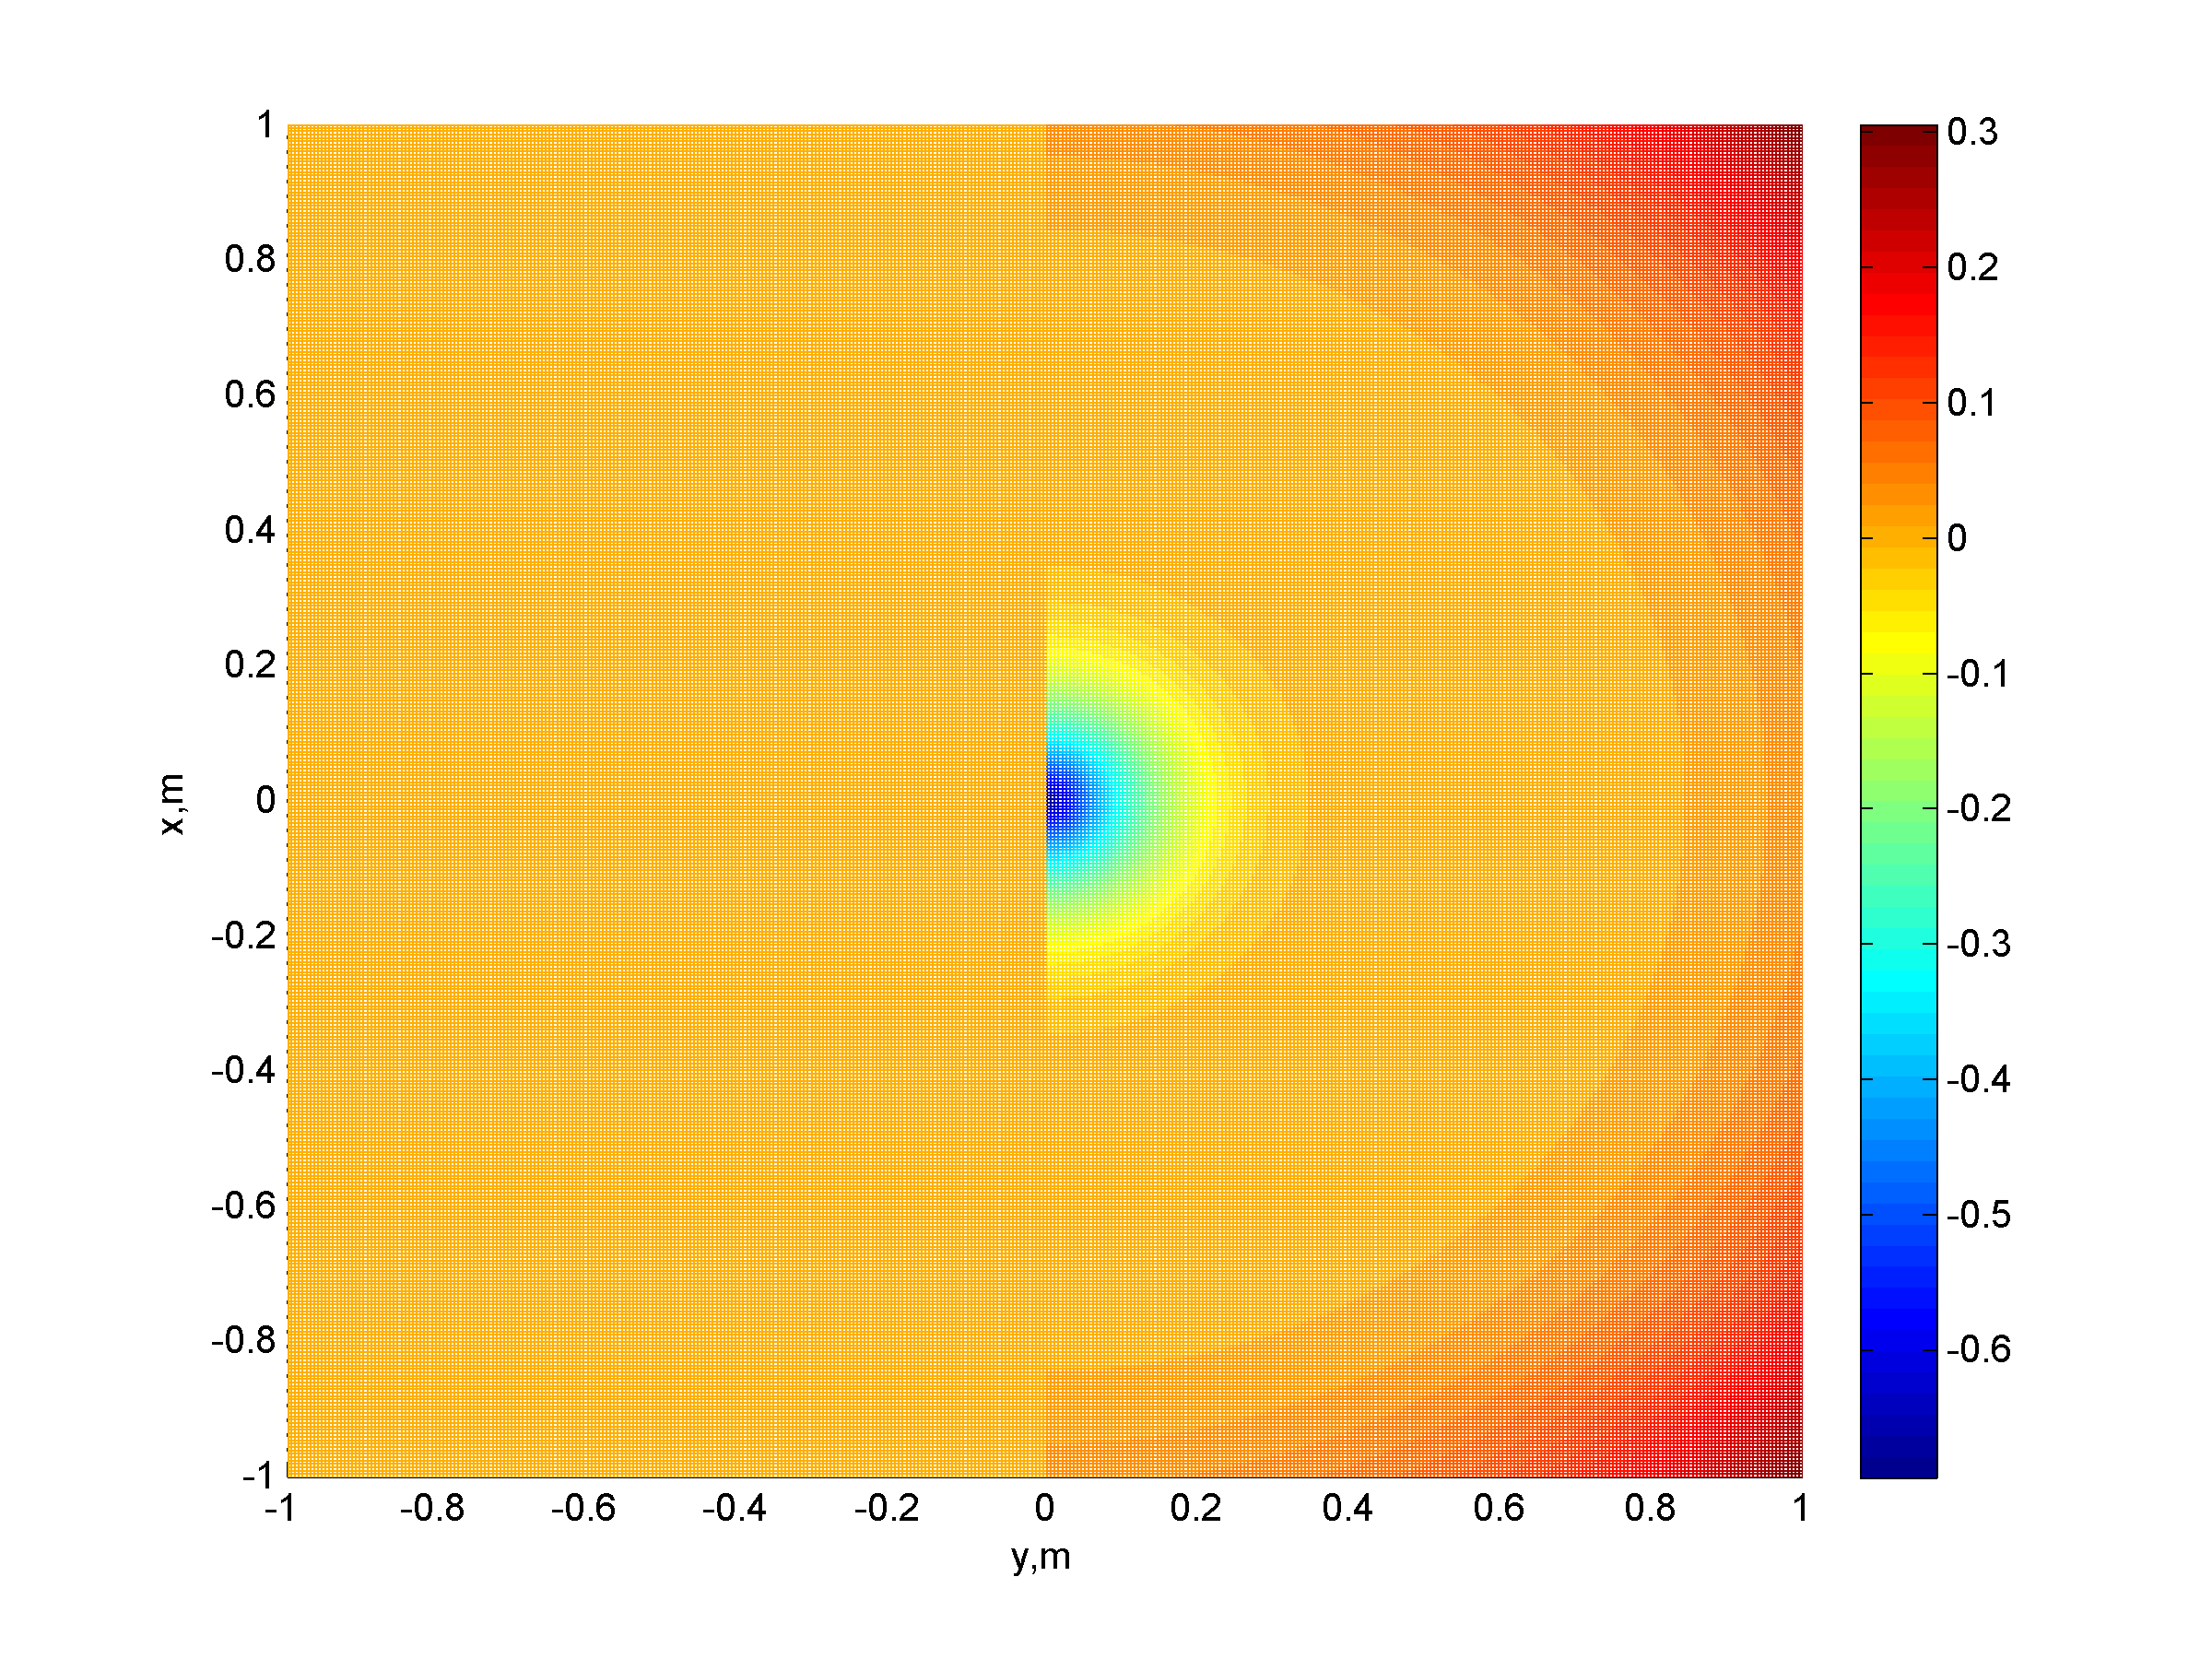
\includegraphics[width=\textwidth]{potential_function.png}}
								\caption{Composite potential field, $f(x)g(x,\psi)$.}
								\label{fig::potential_field}
							\end{figure}
			%In the event that the robot does get stuck in a potential minima, a ``stuck" detection algorithm has been implemented. As the name suggests, this algorithm first detects if the robot is stuck in a local minima of the potential field based on a window of command histories.

			Finally, the command vector $\vec{V}_{L}^{r}$ is transformed into scalar forward and turning rate commands, ${v}_{L}^{r}$ and $\omega_{L}^{r}$, respectively, by the following proportional control scheme:
				\begin{eqnarray}
				\theta_{L}^{r} 			&=& \tan^{-1}\wrap{ \frac{\vec{V}_{c,2}^{L} }{\vec{V}_{c,1}^{L}} } \nonumber\\
				\dot{v}_{L}^{r} 			&=& \beta_{v} \wrap{ \norm{ \vec{V}_{L}^{r} } - v_{L}^{r} } \nonumber \\
				\dot{\omega}_{L}^{r} 	&=& \beta_{\omega} \wrap{ \wrap{ \frac{ \omega_{L}^{r,max} }{\pi} } \wrap{  \theta_{L}^{r} - \theta_{b,z} } - \omega_{L}^{r} }
				\end{eqnarray}
			where $\beta_{v}$ and $\beta_{\omega}$ are proportional-gain tuning parameters; and $\theta_{b,z}$ is the platforms yaw in $O_{0}$. The parameters $\beta_{v}$ and $\beta_{\omega}$ can be viewed as ``update-inertias," as they directly effect the influence of the effect of instantaneous commands on the forward velocity and turning rate of the robot. Furthermore, these gains can be used to low-pass navigation updates to remove jitter cause by command outliers generated from degenerate sensor readings.
				\begin{figure}[t!]
					\centering
					\fbox{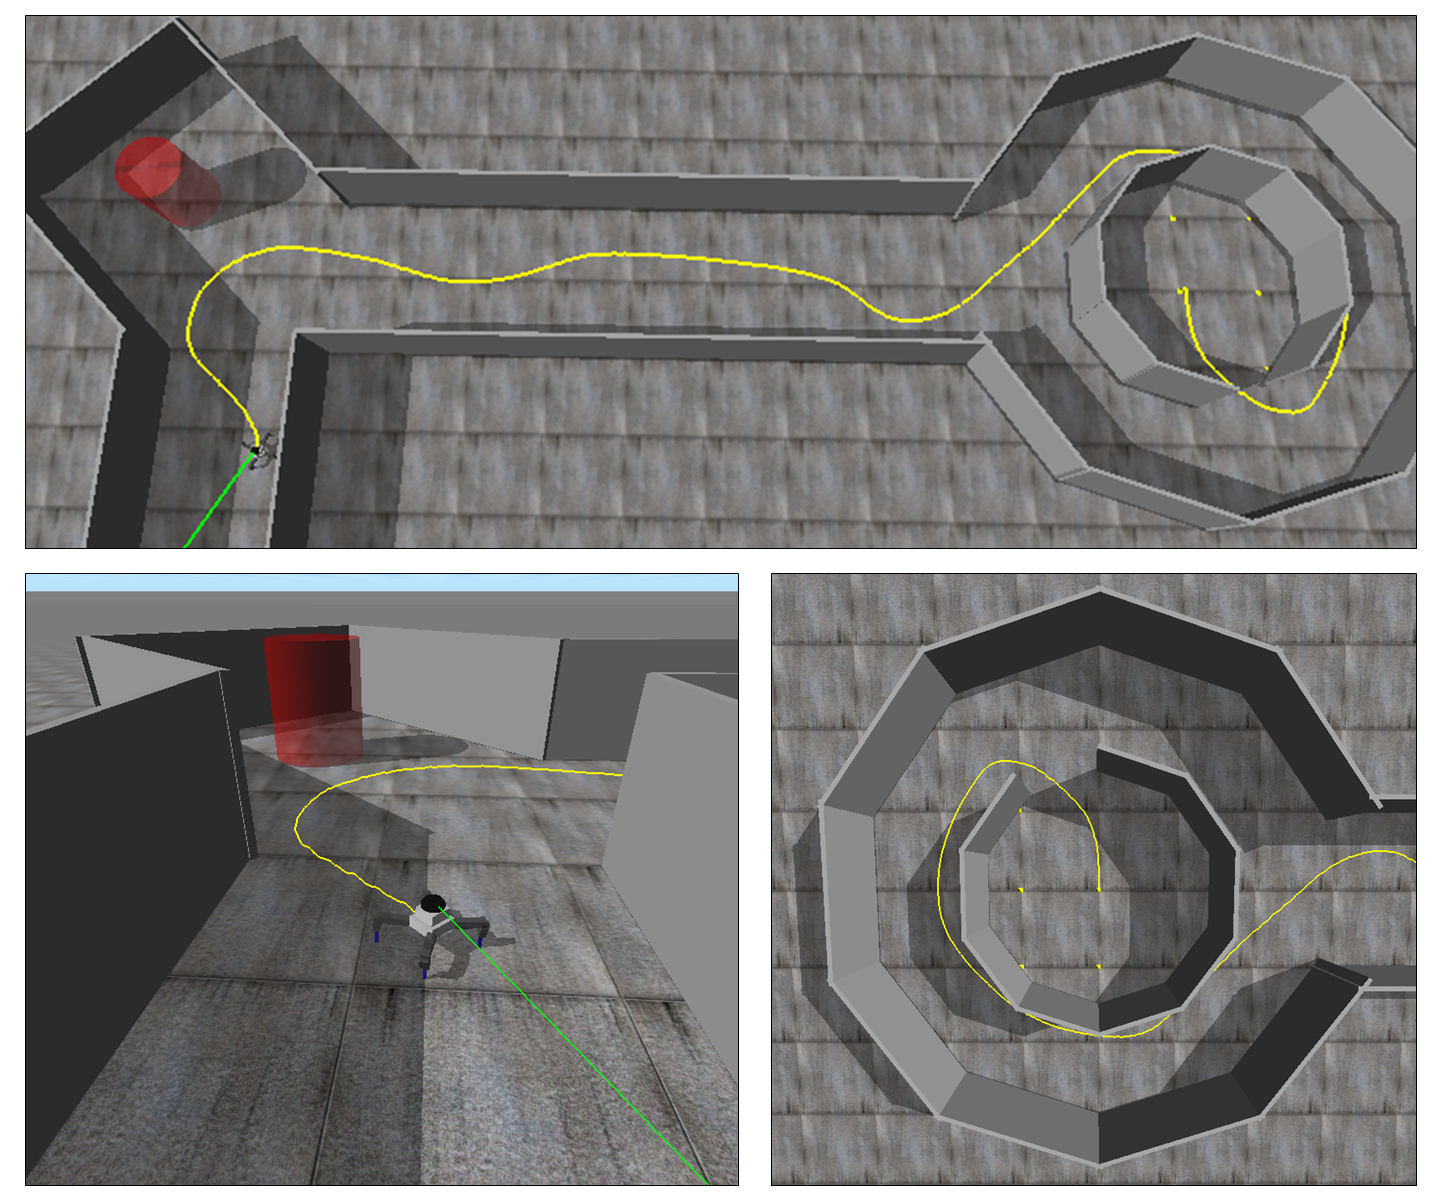
\includegraphics[width=\textwidth]{potential_field_full.png}}
					\caption{Path (shown in yellow) taken by robot through a simulated set of rooms and halls using the LIDAR-based potential fields navigation scheme.}
					\label{fig::potential_field_results}
				\end{figure}

		\subsection{Results of LIDAR-based potential field navigation from simulation}


		\subsection{Incorporation of Camera-based Feature-Tracking}
		
			Camera-based goal tracking is used in conjunction with the aforementioned potential fields navigation scheme to move the platform through an environment while seeking or tracking a particular target. In this case, targets take the the form of features extracted from processed camera data. The robot is guided towards these features using a visual-serving approach. 

			Trackable camera features can be generated in a variety of ways. For the purpose of BlueFoot's navigation, objects with distinct shapes or color have been chosen for tracking so that shape and blob detection algorithms can be employed to detect their positions relative to BlueFoot's camera view range. Namely, Bluefoot's image processing routines make use of the Hough Transform-based shape detection and standard color-blob detection algorithms available from the Open Computer Vision (OpenCV) libraries [Need Hough Ref, Need OpenCV Ref]. Once detected, center-positions of each feature, represented with respect to the 2D camera-viewing frame, are mapped into forward rate and turning commands to control the robot towards the relative location of the feature. These camera-based commands are then mixed with the outputs of the potential-fields navigation controller to form a hybrid navigation control law.

			In this visual-servoing approach, features are used to control the robot in a way that is agnostic of the type of feature being tracked. Namely, this approach relies on the relative position of the center of each features, represented as a pixel-position, $p_{Im} = [u,v]^{T} \in Z^{2}$ in the 2D image frame, $O_{Im}$, and a relative size, $r$, measured in pixels. In the case of circular features, for example, $r$ is represent the radius of the detected circle. For color-blob features, $r$ represents the radius of a circle which fully inscribes the colored object.

			For the purpose of target tracking, it is desired that the robot's forward speed be controlled such that is proportional to $r$. Namely, it is desired that the robot stop when it becomes close to the target object, and move faster when the feature is in sight but the robot is further away. The position of the feature's center us used to control the robot's turning rate, as well as the commanded pitch of the robot's trunk, $\theta_{b,x}^{r}$. Trunk articulation important during feature tracking routing as it aids in keeping the tracked-target objects centered in the image frame. Provided that the target is moving slower than the what the system can achieve, this will ensure the target remains in sight at all times.

			A separate set of navigation commands, $v_{C}^{r}$ and $\omega_{C}^{r}$; and an additional body-pitching command, $\theta_{b,x}^{r}$,  are generated from an extracted feature location, $p_{Im} = [u,v]^{T}$ as follows: 
				\begin{eqnarray}
					v_{C}^{r} 			& = & v_{C}^{r,max} \wrap{ 1 - e^{ -c_{r} \wrap{ r-r_{min} }^{2} } } 	\nonumber 	\\
					\omega_{C}^{r} 	& = & \omega_{C}^{r,max} \wrap{\frac{ w_{Im} - 2 u  }{ w_{Im} } }		\nonumber 	\\
					\theta_{b,x}^{r}	& = & \theta_{b,x}^{r,max} \wrap{ \frac{ 2 v - h_{Im} }{ h_{Im} } } 		
				\end{eqnarray}
			where $v_{C}^{r,max}$, $\omega_{C}^{r,max}$ and $\theta_{b,x}^{r,max}$ are the maximum magnitude of forward velocity, turning rate, and body-pitching commands, respectively; $c_{r}$ is a sensitivity parameter; $r_{min}$ defines a minimum feature size which will result in the administration of a zero velocity command to the platform (and thus the distance from the feature at which to halt forward motion); and $w_{Im}$ and $h_{Im}$ define the width and height, respectively, of the image being processed. Having now established a formulation for how a single, distinct, feature is used to guide the platform towards a target, a means of fusing the LIDAR-based command signals and the camera-based command signals will be defined.

			The composition of this hybrid command technique is motivated by two key subtasks: to use the potential fields algorithm during a wandering phase, when a target object is not in sight; and to guide the robot towards the goal once in sight, allowing the camera-based tracking commands to have a greater influence on system navigation (through the variables $v^{r}$ and $\omega^{r}$) as the platform becomes closer to the desired target. A straight-forward way to achieve this is to use the relative size. $r$, of tracked target features in the image frame. With this in mind, a simple command mixture scheme has been defined as follows:
			\begin{eqnarray}
				v(r) &\equiv&
				\begin{cases}
				e^{ -c_{mix} \wrap{ r - r_{mix}}^{2} } 	& \text{if } r < r_{mix}	\\
				1											& \text{else}
				\end{cases}
								\nonumber \\
						\left[\begin{array}{c} v^{r} 	\\ \omega^{r} 		\end{array} \right] &=& 	
				v(r)	\left[\begin{array}{c} v^{r}_{C}\\ \omega^{r}_{C} 	\end{array} \right] + 
				(1-v(r))\left[\begin{array}{c} v^{r}_{L}\\ \omega^{r}_{L} 	\end{array} \right] 
			\end{eqnarray}
			where $c_{mix}$ is a sensitivity parameter; and $r_{mix}$ defines the processed-feature size which will grant full navigation control to the camera-based navigation scheme. The reasoning for such a scheme involves a heuristic approach to obstacle aversion, which assumes that when the platform is further away from a goal, there is a higher probability that it will encounter an obstacle. Conversely, when the goal becomes closer to the platform, it assumed that the number of obstacles between the robot and the target decreases, making it safe to shift full priority to reaching the goal from the current position. It is defined that if a feature is now found withing the current view, then it is considered to be of size $r=0$.

		\subsection{Hybrid Potential-Fields Navigation Results}
		*NEED RESULTS*



	\section{Rough Terrain Navigation}

		\subsection{Terrain Mapping with 3D Point-clouds}
			
			\subsubsection{3D Point Cloud generation from 2D scans}
				\begin{figure}[h!]
					\centering
					\caption{Need sensor sweep diagram.}
					\label{fig::sensor_sweep}
				\end{figure}
				The BlueFoot platform has the ability to compose 3D point clouds from a series of swept 2D LIDAR scans in conjunction with a trunk orientation estimates, $\hat{\theta}_{b}$, which is generated using an EKF. LIDAR articulation is achieved by slowly pitching the trunk over some angular range while keeping the platform's feet ridgedly planted. Sweeping range is limited by the kinematic-feasibility of each trunk pose that must be reached during a sweep. Given a particular set of foot and body location, kinematic feasibility is validated using the inverse kinematics solution described in Section \ref{sec::inverse_position_kinematics}. A single 2D scan is taken at each pose within the body-sweep trajectory. The newly acquired scan is transformed from the LIDAR sensor frame, $O_{L}$, to the world frame by a homogeneous transformation $H^{L}_{0}$ which is defined as follows
					\begin{equation}
						H^{L}_{0} = H^{L}_{b} H^{b}_{0}
						\label{eq::world_to_sensor}
					\end{equation}
				where $H^{b}_{0}$ is a transformation from $O_{0}$ to the trunk frame $O_{b}$, as defined in Chapter \ref{ch::system_modeling}; and $H^{L}_{b}$ defines a transformation from the frame $O_{b}$ to the LIDAR frame, $H^{L}_{b}$. $H^{L}_{b}$ is necessary for knowing the position of the LIDAR head with respect world frame, as the sensor itself has some offset and rotation relative to the robot's body. Each 2D point from $x_{i} \in \emph{S}$ from the initial scan, $\emph{S}\subset \Re^{2}$, can then be transformed into a 3D scan segment, $\bar{S}_{j}$, in $O_{0}$ by:
					\begin{equation}
						\left[
							\begin{array}{c}
								y_{i,j} \\ 1
							\end{array}
						\right]
					 = H^{L}_{b} H^{b}_{0}	
						\left[
							\begin{array}{c}
								x_{i} \\ 0 \\ 1
							\end{array}
						\right] \forall x_{i} \in \emph{S}
						\label{eq::scan_to_segment}
					\end{equation}
				where $y_{i,j} \in \bar{S}_{j}$ is a point withing the 3D \Jth scan segment $\bar{S}_{j} \subset \Re^{3}$. After the sweeping routine is complete, 3D scan segments are composed into a final point cloud, $\bar{S}$ by:
				\begin{equation}
					\bar{S} = \cup_{j=1}^{N_{s}} \bar{S}_{j}
				\end{equation}
				where $N_{s}$ defines the number of scans taken during the sweeping routine.
				For the sake of simplicity, it is assumed that the trunk's position, $p_{b}$, is fixed (system is completely ridged) during a swept-scan routine. In the results to be presented, this seems to be a reasonable assumption given that the platform is at rest and the trunk is pitched sufficiently slowly over the angular sweeping range. A slow sweep rate ensures that perturbations caused by vibrations incurred by trunk rotation and foot-slip are small, and thus does not cause for significant deviations in LIDAR scan points.
					\begin{figure}[h!]
						\centering
						\fbox{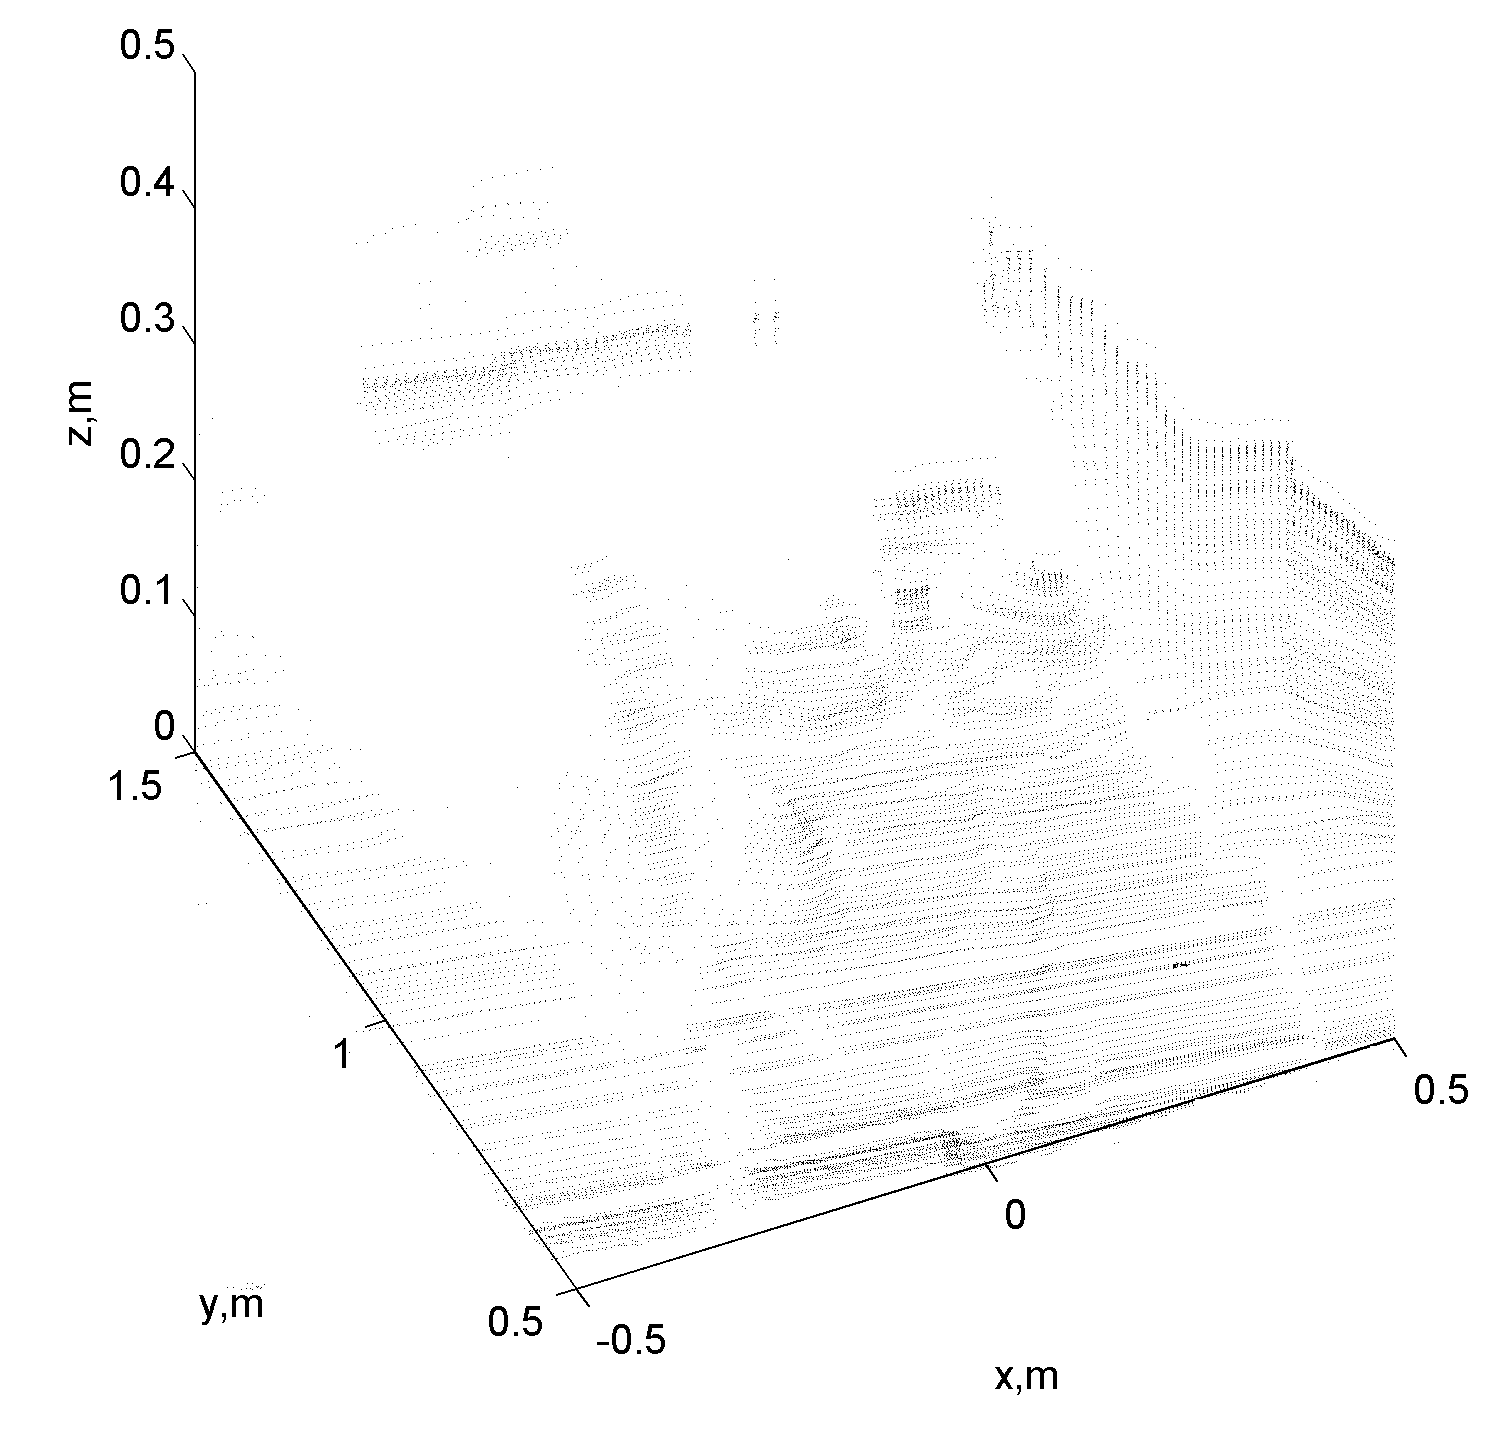
\includegraphics[width=\textwidth]{terrain_pcd3_cleaned.png}}
						\caption{Original 3D point-cloud of terrain patch.}
						\label{fig::pointcloud_terrain_patch}
					\end{figure}


			\subsubsection{Height-map from 3D point cloud}
				
				3D point clouds can be transformed into height-map representations. These representations are convenient for use in planning as they can be converted into discrete cost-maps in a straightforward way. These height-maps are generated by populating the elements of a matrix  $M\in \Re^{n\times m}$ with the $z$ components of points which exist within discretized $W\times D$ region within the original 3D point cloud. The location and size of this regions would have to be determined with some auxillary detection process which 1) determines that the area has high terrain variation, and 2) determines the bounding region where this patch of rough-terrain exits. Once this regions is determined, the 3D cloud is divided into $(nm)$ sub-divisions, each of which covers a $(W/m) \times (D/n)$ area. Each \Ith, \Jth element of $M$ is then populated with the highest point (larger  $z$ component) within each  \Ith, \Jth subdivision. Depending on the density of the 3D point cloud, this process has the potential to produce relatively sparse height-map. To deal with this, a dilation and smoothing routine is used to complete the height-map conversion process. During dilation, each non-zero height element within the map is expanded into a region around the exiting element until. This process is performed until a semi-uniform map is produced with minimal gaps between non-zero height elements. Finally, a median filter is applied to the dilated height-map to produce smooth transitions between height elements.
				\begin{figure}[t!]
					\centering
					\fbox{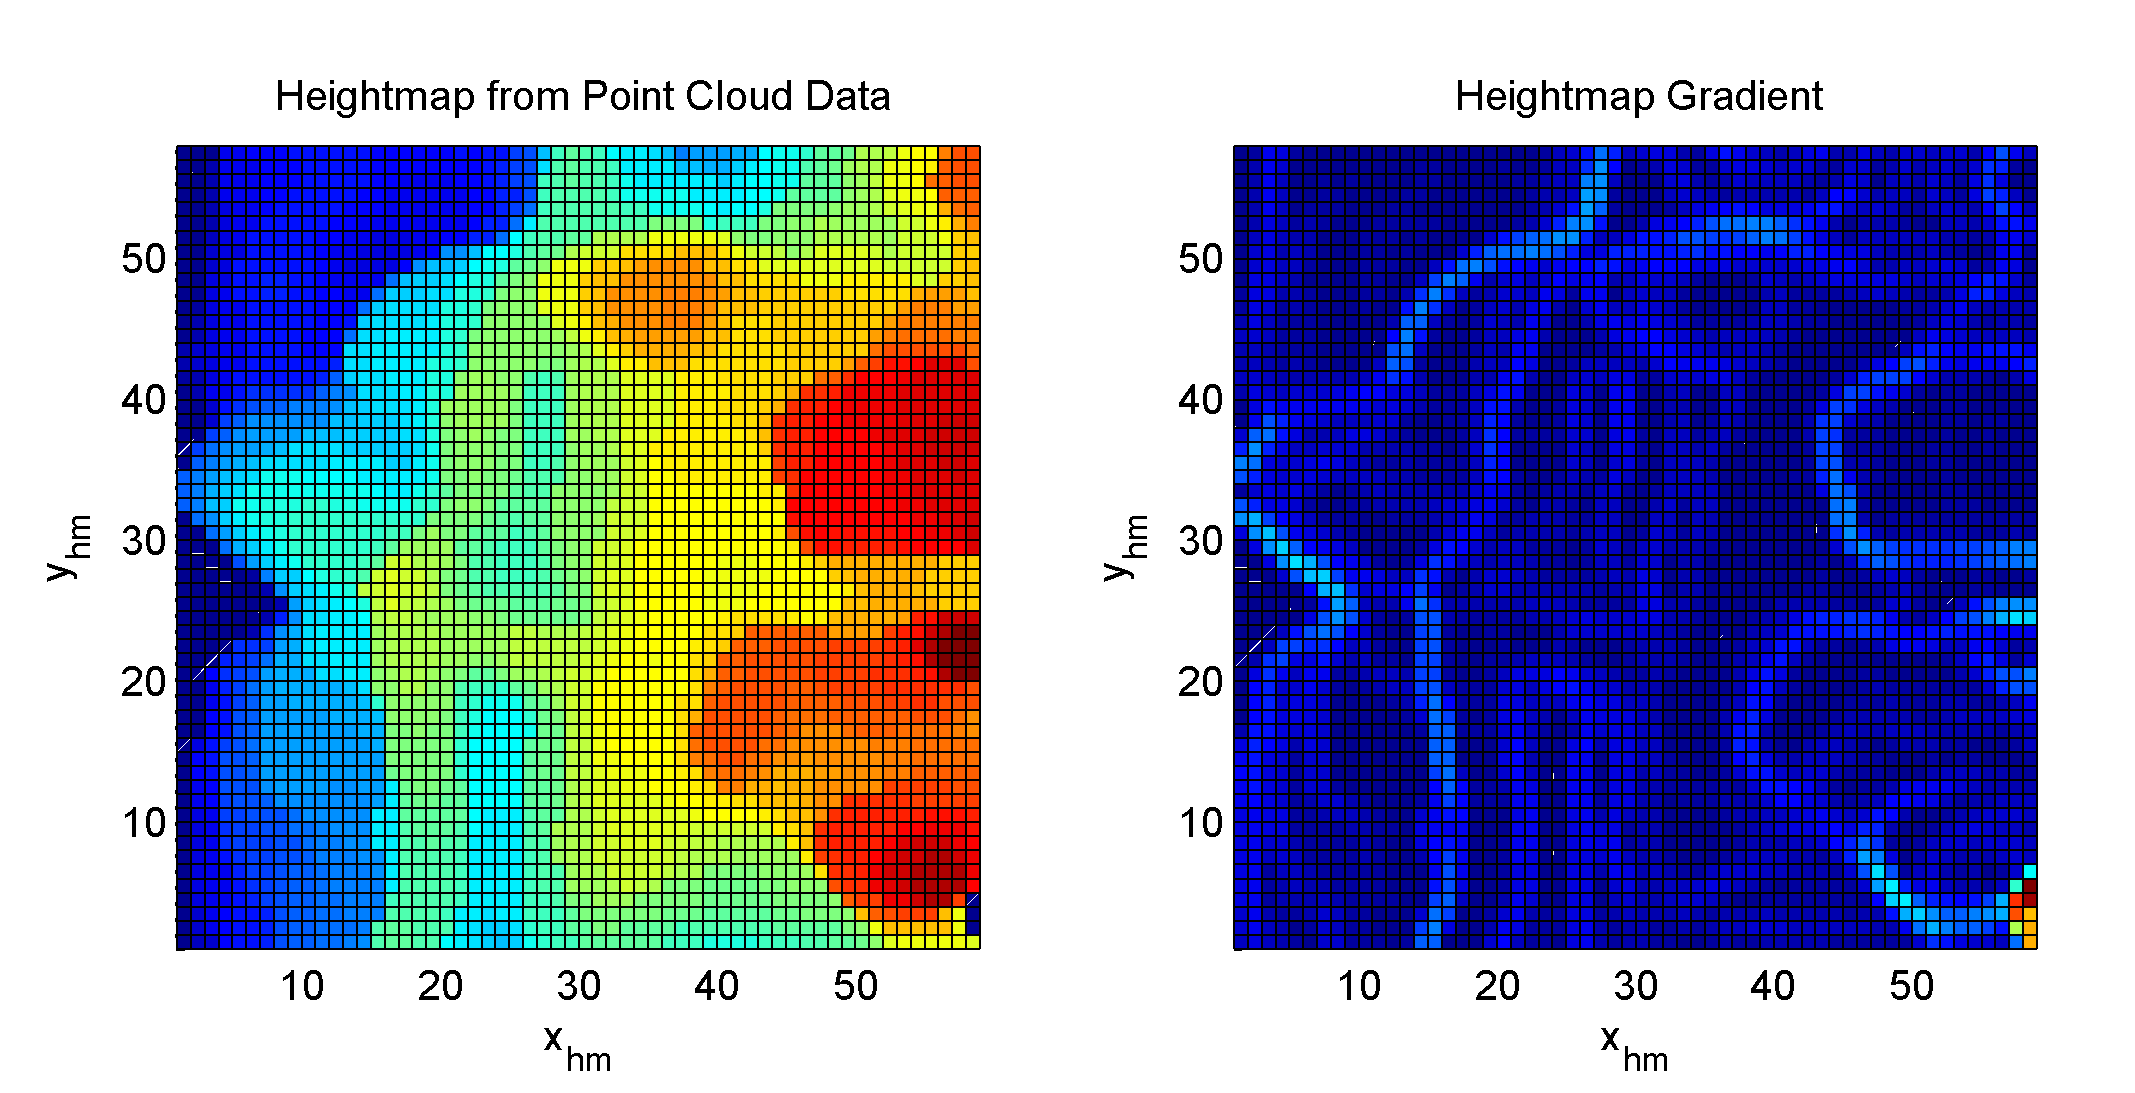
\includegraphics[width=\textwidth]{terrain_grad_crop.png}}
					\caption{Relative height-map \emph{(left)} and its corresponding gradient \emph{(right)}.}
					\label{fig::heightmap_terrain_patch}
				\end{figure}
				\begin{figure}[h!]
					\centering
					\fbox{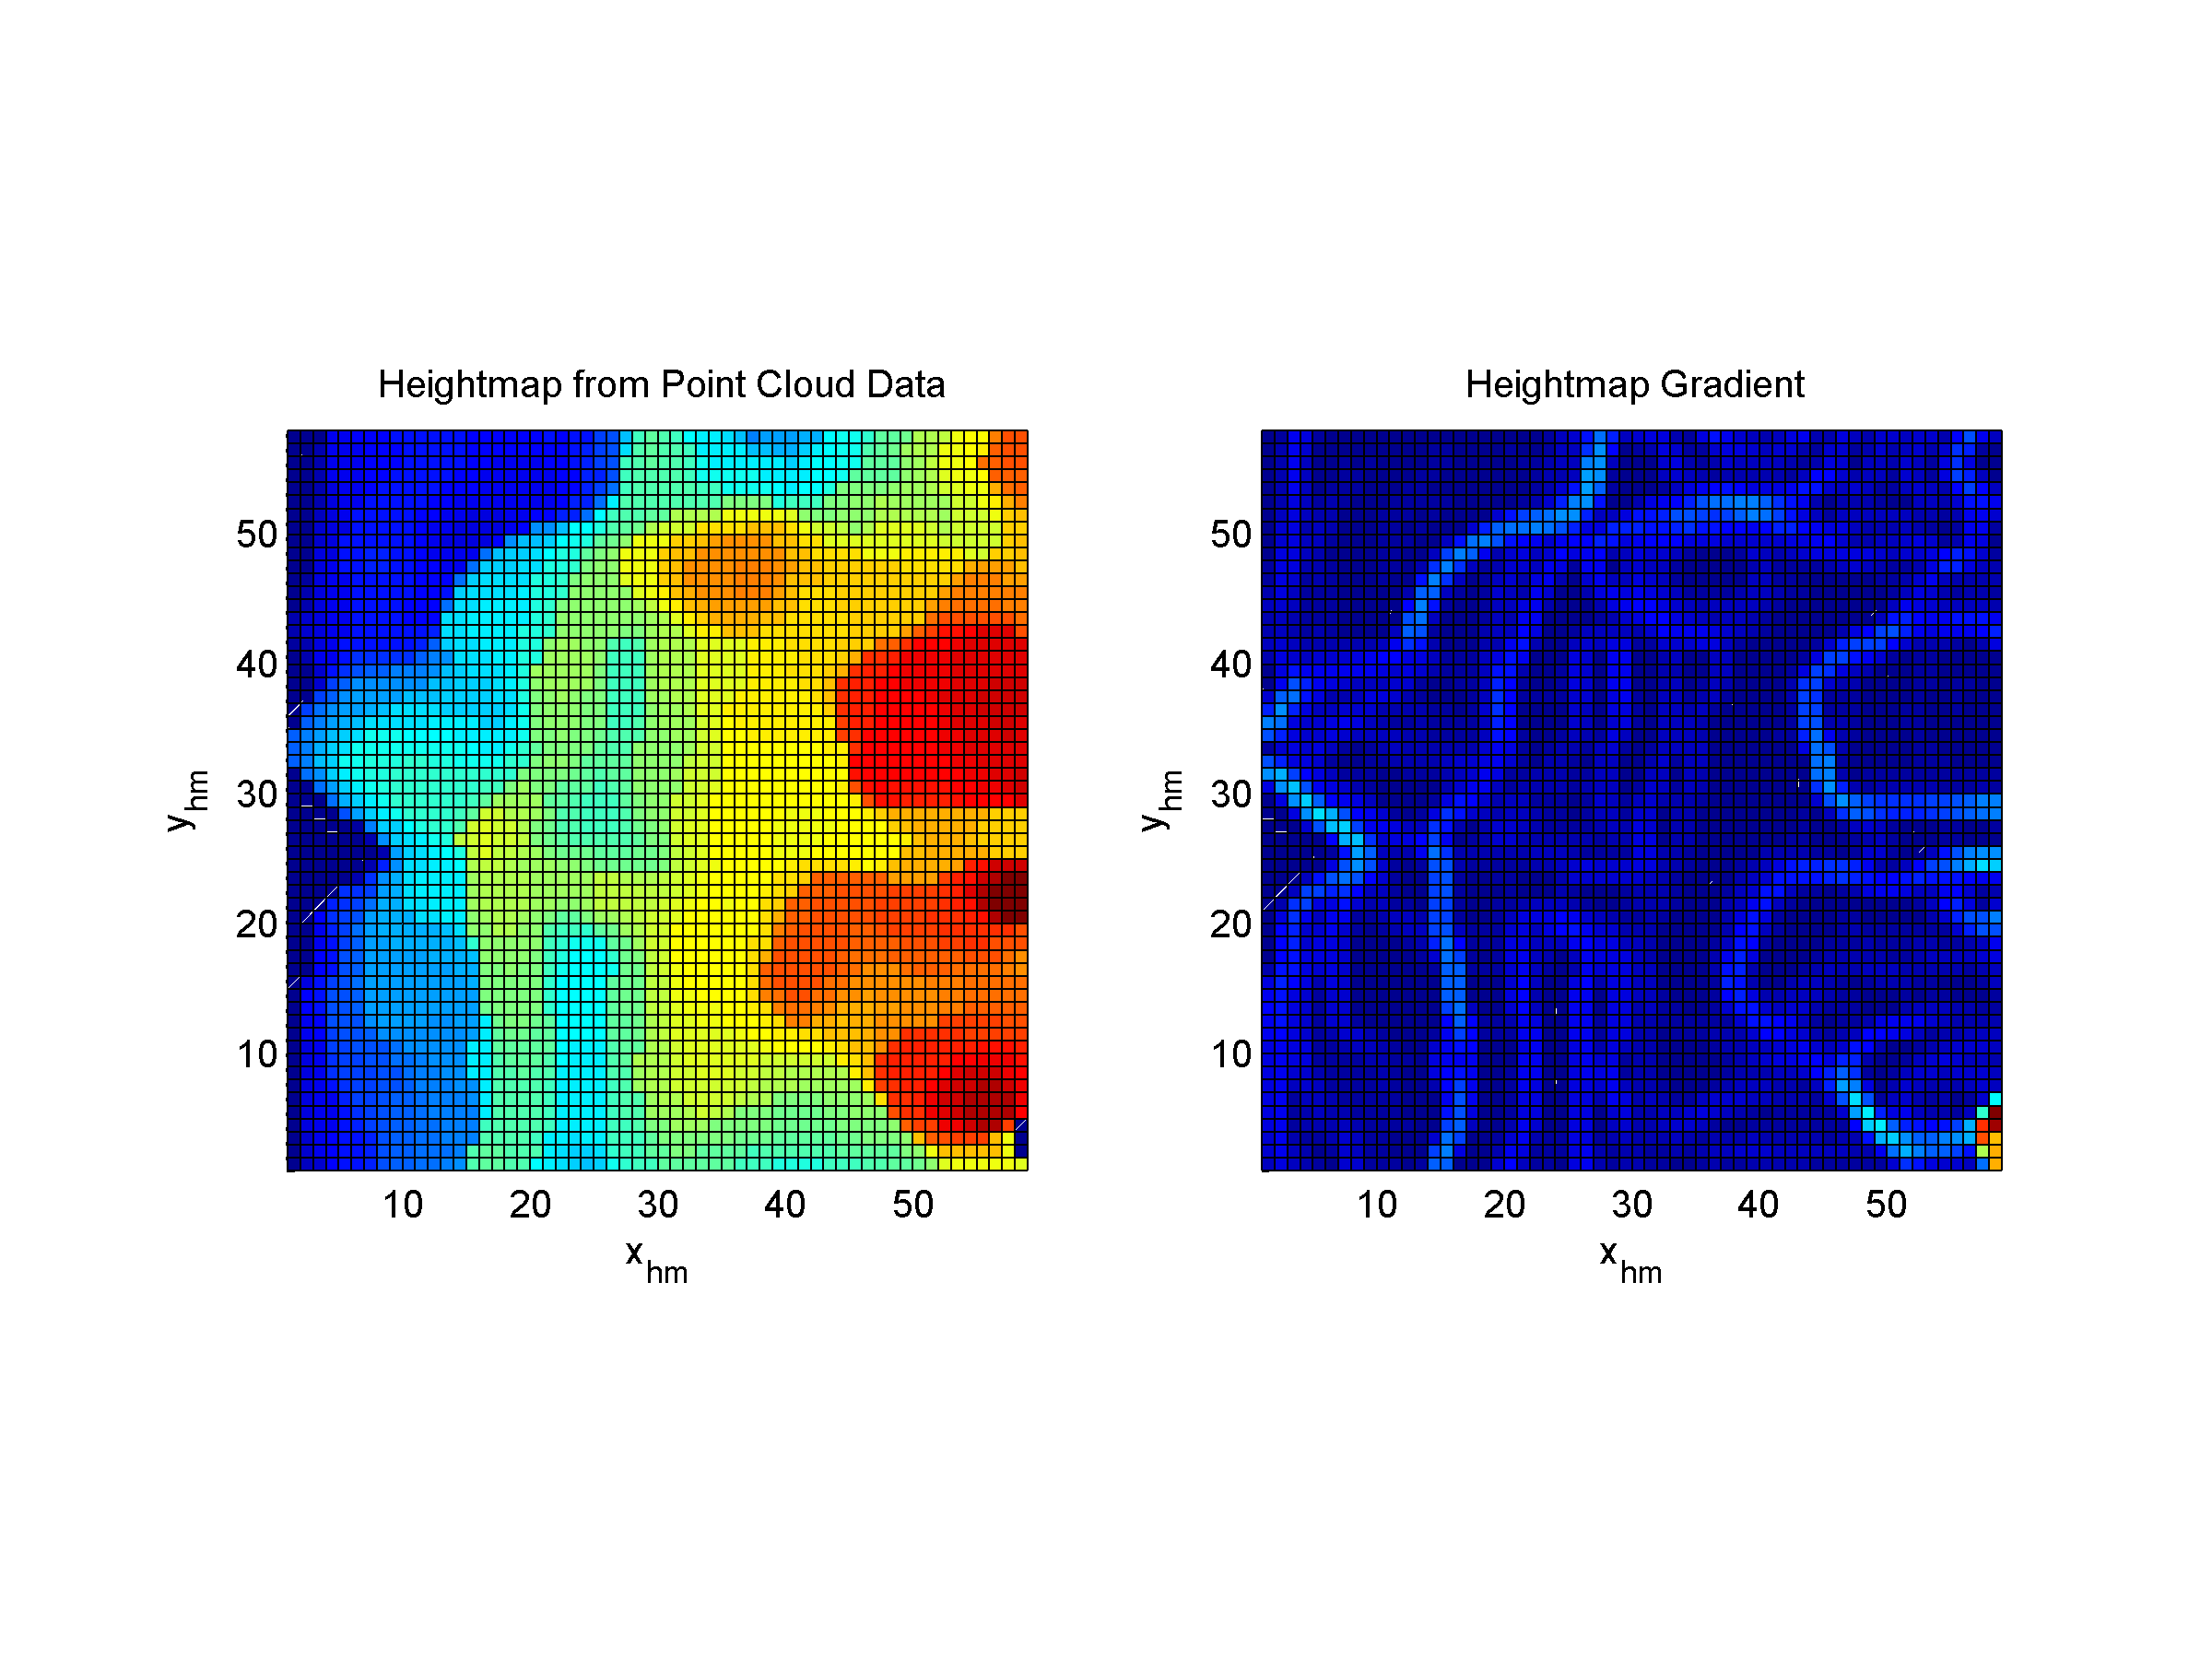
\includegraphics[width=\textwidth]{terrain_4545.png}}
					\caption{Height-map showing terrain variation in the $z_{hm}$ direction.}
					\label{fig::heightmap_terrain_patch_ortho}
				\end{figure}							
			
			The full 3D point cloud to height-map conversion algorithm is summarized as follows:


			\subsubsection{Surface Reconstruction}


		\subsection{Proposed Methods for determining the existence of Rough Terrain}

		\subsection{Foot-placement planning}



	%%%%%%%%%%%%%%%%%%%%%%%%%%%%%%%%%%%%%%%%%%%%%%%%%%%%%%%%%%%%%%%%%%%%%%%%%%%%%%%%%%
%%% Conclusion
%%%%%%%%%%%%%%%%%%%%%%%%%%%%%%%%%%%%%%%%%%%%%%%%%%%%%%%%%%%%%%%%%%%%%%%%%%%%%%%%%%
\chapter{Concluding Remarks}

This thesis has provided a comprehensive summary of the design and control of the BlueFoot quadruped platform. Namely, BlueFoot's structural configuration; associated component devices; gait and stability control; and related navigation control mechanisms have been described in detail. Results, both simulated and actual, have been provided about the performance of each control technique used in operating the BlueFoot platform.

Future work involving the design improvements upon the existing BlueFoot platform will be 

Future work involving the control of the BlueFoot platform will mainly deal with methods and supporting algorithms for traversing irregular terrain.  One such algorithm will involve the location and classification of rough terrain regions. Such an algorithm will be used to deduce whether or not an area of terrain is of high irregularity; as well as whether or not the terrain is traversable or needs to be traversed in order to reach a goal location. Then, the associated area will be mapped and the surface reconstruction mechanisms details in this thesis will be employed. Finally, adaptive footstep planning over the terrain will be carried out. As opposed to planning over a static terrain map, it is desired that BlueFoot continuously maps and re-plans a path for navigation over arbitrary terrain. Although adaptive planning is not always necessary, there are many environmental situations wherein an adaptive terrain traversal approach is required. For instance, one such situation occurs when the robot can only partially perceive the terrain ahead of it from its current vantage point. This would occur if the terrain being mapped was taller than the effective height of the LIDAR laser head, and the sensor could not be articulated in such a way that the entirety of an immediate terrain patch was viewable. In this case, current implementations for surface reconstruction utilize approximations for terrain beyond that of which is immediately viewable by the robot platform, such as those described in \cite{other dudes}. Instead, it is desirable to have a routine which navigates the robot based on a continuously updated terrain map. This would require that BlueFoot executes a coordinate set of motions which allow it to articulate its LIDAR sensor will walking to map the immediate terrain. From this whole-body motion planning problem. The solution to such a problem would need to address a way of combining optimal and body-motion trajectory planning to achieve both the aforementioned subtasks in concert. Additionally, the problem of online terrain mapping would require that the platform can accurately localize itself upon the known portions of the terrain while incorporating new terrain-map data, extending this study in the realm of 3D Simultaneous Localization and Mapping.
%%%%%%%%%%%%%%%%%%%%%%%%%%%%%%%%%%%%%%%%%%%%%%%%%%%
\bibliographystyle{unsrt}
\bibliography{refs}
\end{document}

